\documentclass[a4paper, oneside]{book}
\usepackage[a4paper, total={6in, 9.5in}]{geometry}
\usepackage{blindtext}
\usepackage{titlesec}
\usepackage{graphicx} % Required for inserting images
\usepackage{array}
\usepackage{helvet}
\usepackage{ragged2e}
\usepackage{amsmath}
\usepackage{float}
\usepackage{chngcntr}
\usepackage{tabularx}
\usepackage{indentfirst} % para que indente el primer parrafo de cada seccion
\usepackage[hidelinks]{hyperref} % para crear links de refs
%\usepackage{refcheck} % para activar checkeo de citas no usadas
\usepackage[table]{xcolor}
\graphicspath{{images/}} %configuring the graphicx package

% para que numere las imagenes por secciones y no capitulos
\counterwithin{figure}{section}

% definiciones para la bibliografia
\nocite{*}
\bibliographystyle{IEEEtran}

% para no solapar el texto en el indice de imagenes
\makeatletter
\renewcommand*\l@figure{\@dottedtocline{1}{1em}{3em}}
\makeatother

% definiciones de nombres
\renewcommand{\chaptername}{Capítulo}
\renewcommand{\contentsname}{Tabla de contenido}
\renewcommand{\listfigurename}{Índice de imágenes}
\renewcommand{\figurename}{Figura}
\renewcommand{\bibname}{Bibliografía}

% definiciones de colores
\definecolor{test_header_color}{HTML}{D5E5FF}
\definecolor{precond_header_color}{HTML}{8EC0EE}

% definiciones de formato de tablas para tests
\newenvironment{testtableformat}{
    \sffamily \small \begin{center} \begin{tabular}{|p{3cm}|p{11.5cm}|} 
}{ 
    \end{tabular} \end{center} \normalsize \normalfont
}

% profundidades de la tabla de contenido
\setcounter{tocdepth}{5}
\setcounter{secnumdepth}{5}

% https://manualdelatex.com/tutoriales/estructura-de-un-documento
% https://www.overleaf.com/learn/latex/Learn_LaTeX_in_30_minutes
% https://docs.aspose.com/tex/es/java/latex-math-subscripts-superscripts/

\title{Proyecto Integrador}
\author{\\Franco Vaira \\ Antonio Tolay}
\date{Diciembre 2024}

\makeatletter 
\let\newtitle\@title
\let\newauthor\@author
\let\newdate\@date
\makeatother

\begin{document}

% choreado de: https://es.overleaf.com/project/67ef0bcc06f70ab44f8fa36c
% se pueden sacar otras cosas

\thispagestyle{empty}
\begin{center}
    \begin{figure} \begin{minipage}{.42\textwidth}
        
\includegraphics[scale=0.11]{images/logo_unc.png}
    \end{minipage}
    \hfill
    \begin{minipage}{.6\textwidth}
        \vspace{0.05cm}
        
\includegraphics[scale=0.28]{images/logo_FCEFyN.png}
    \end{minipage}\end{figure}
    
    \vspace{1cm}

    \begin{LARGE}
        \textbf{Universidad Nacional de Córdoba} \\
        \vspace{0.3cm}
        Facultad de Ciencias Exactas, Físicas y Naturales \\
        \vspace{0.3cm}
        Departamento de Computación \\
    \end{LARGE}
    
    \vspace{2cm}

    \begin{Huge}
        \textbf{\newtitle} \\
        \vspace{0.3cm}
        Robot omnidireccional \\
    \end{Huge}

    \vspace{2.5cm}
    
    \begin{Large}
        \textbf{Autores:} \newauthor \\
        \vspace{1.0cm}
        \textbf{Profesores:} \\
        PhD. Ing. Orlando Micolini \\
        Ing. Luis Orlando Ventre \\
        \vspace{1cm}
        Córdoba, Argentina. \\
        \newdate
    \end{Large}
\end{center}

\tableofcontents
\newpage
\listoffigures

% fuentes de esta seccion
% https://www.sewio.net/uwb-technology/two-way-ranging/

\newpage
\chapter*{Resumen}

En el presente proyecto se detalla el proceso de diseño y puesta en marcha de un sistema ciberfísico el cual usa cómo base la estructura del robot móvil omnidireccional Hermes III, desarrollado como proyecto integrador de la carrera de grado Ingeniería en Computación en la Facultad de Ciencias Exactas, Físicas y Naturales.

Este proyecto está centrado en el estudio del comportamiento y modelado de un sistema compuesto por varios robots que deben seguir cada uno una trayectoria de un conjunto de trayectorias posibles calculadas previamente con algoritmos de planificación. Cada robot cuenta con un sistema de control compensado para corregir errores en los movimientos.

Partiendo de un conjunto de trayectorias prefijadas para cada robot, se modela el sistema mediante el uso de Redes de Petri y el entorno en el que se mueven los robots se considera particionado en regiones, y cada región del mapa se modela como un lugar en la Red de Petri. Para evitar colisiones se establecen regiones con capacidad finita donde no pueden pasar por ellas más de un robot al mismo tiempo, de modo que si un segundo robot quiere pasar por esa misma región deberá esperar.

Por otra parte, nos interesa lograr que el sistema pueda ubicar al robot con precisión dentro del plano, de modo que se utilizan herramientas como el Filtro de Kalman para lograr una estimación de la posición actual en base a la fusión de lecturas de los diversos sensores.
\newpage
\chapter*{Motivación}

En el ámbito industrial, los robots autónomos han demostrado una capacidad sobresaliente para ubicarse en el espacio y resolver conflictos emergentes de manera eficiente. Sin embargo, dichos sistemas presentan barreras significativas para el acceso por parte del usuario final y carecen de una documentación adecuada, lo que limita su integración en sectores más amplios que no sean exclusivamente industriales. Este trabajo se propone investigar y desarrollar un prototipo de robot autónomo accesible y versátil, diseñado para operar en distintos ámbitos como la medicina, el rescate y el uso doméstico. La motivación principal de este proyecto radica en democratizar la tecnología robótica, promoviendo su uso en contextos donde actualmente es limitada o inexistente.

El desarrollo de robots autónomos enfrenta un desafío importante debido a los elevados costos asociados con los sistemas existentes. Sin embargo, los avances tecnológicos recientes han abierto la posibilidad de diseñar prototipos funcionales utilizando componentes disponibles en el mercado, con un diseño simplificado y económico que minimiza el número de piezas mecánicas. Esto contribuye no solo a la reducción de los costos iniciales, sino también a una disminución significativa en los requerimientos de mantenimiento, lo que hace que la solución sea más sostenible y escalable en el largo plazo.

El estudio se centra en el comportamiento y modelado de sistemas compuestos por múltiples robots, los cuales seguirán trayectorias calculadas previamente mediante algoritmos de planificación de rutas. Esto permite investigar técnicas avanzadas de navegación autónoma y coordinación, además de abordar desafíos clave como la prevención de colisiones y la optimización de movimientos en entornos compartidos. La implementación de estas técnicas en un prototipo funcional representa una contribución relevante al campo de la robótica móvil, con un alto potencial para ser aplicada en diversos escenarios prácticos.

En resumen, este proyecto responde a la necesidad de desarrollar soluciones robóticas accesibles y eficientes que puedan ser adoptadas en sectores variados y de forma práctica. La combinación de avances tecnológicos con un enfoque en la reducción de costos y la simplificación del diseño no solo busca avanzar en el conocimiento técnico, sino también facilitar la integración de esta tecnología en contextos donde actualmente no está disponible, ampliando así su impacto y utilidad.

% En la industria existen robots autónomos que son capaces de ubicarse en el espacio donde se mueven y poder resolver conflictos emergentes. Estos robots no suelen ser de disponibilidad a un usuario final ni tampoco hay mucha documentación al respecto, por lo que una de nuestras mayores motivaciones es investigar y desarrollar un robot de similares características que pueda ser utilizado en diversos sectores, como ser medicina, rescate, doméstico, etc.

% Al mismo tiempo es importante notar que los robots ya existentes tienen un alto costo, pero por otro lado la tecnología ha avanzado lo suficiente para que el proyecto sea factible y accesible. Nos motiva lograr un prototipo funcional construido con componentes de alta disponibilidad en el mercado, de bajo costo, y con pocas piezas mecánicas, disminuyendo así el mantenimiento requerido.

% En un nivel más alto este trabajo se centra en el estudio del comportamiento y modelado de un sistema compuesto por varios robots que tienen que seguir cada uno una trayectoria calculada previamente utilizando algoritmos de planificación de rutas.
\chapter{Objetivos}

\section{Objetivos principales}

\begin{itemize}
    \item Lograr construir un prototipo que se mueva por el espacio de modo autónomo.
\end{itemize}


\section{Objetivos secundarios}

\begin{itemize}
    \item Implementar un sistema de locomoción omnidireccional de 4 ruedas.
    \item Desarrollar un sistema de control capaz de corregir los errores del robot al desplazarse.
    \item Implementar una interfaz de usuario para control y monitoreo.
    \item Lograr una comunicación bidireccional con el robot.
\end{itemize}
\subsection{Requerimientos}

En esta iteración abordaremos los siguientes requerimientos funcionales:

\begin{center}
    \begin{tabular} {
        | >{\centering\arraybackslash}m{1cm}
        | >{\centering\arraybackslash}m{13cm} |}
        \hline \rowcolor{test_header_color}
            ID & Descripción \\
        \hline
            RF4 & El robot debe poder realizar trayectorias en línea recta y curvas. \\
        \hline
            RF6 & El robot debe recibir y enviar información mediante comunicaciones inalámbricas. \\
        \hline
            RF8 & Debe poder ubicarse al robot en el plano de forma precisa. \\
        \hline
    \end{tabular}
\end{center}

   Por otra parte, el requerimiento no funcional que abordaremos es:

\begin{center}
    \begin{tabular} {
        | >{\centering\arraybackslash}m{1cm}
        | >{\centering\arraybackslash}m{13cm} |}
        \hline \rowcolor{test_header_color}
            ID & Descripción \\
        \hline
            RNF1 & Debería tener tiempos de respuesta aceptables para el buen funcionamiento del sistema de control. \\
        \hline
    \end{tabular}
\end{center}
\chapter{Análisis de riesgos}

Para el análisis de los riesgos del proyecto, se ha decidido utilizar la estrategia de Mitigación y Gestión de Riesgos, conocido por sus siglas en inglés como RMMM (Risk Mitigation, Monitoring and Management). Para llevar a cabo cada una de las tareas anteriormente mencionadas, se ideará un plan de prevención, un plan de monitorización y un plan de contingencia respectivamente.

Se consideran riesgos aquellas situaciones que, en caso de suceder, afectan negativamente determinados aspectos del proyecto. Por esta razón es importante identificarlos con anticipación para mitigarlos.

El plan de prevención intenta ser un escudo para mantener la cantidad de riesgos latentes al mínimo y que no logren materializarse, por lo que su objetivo es entorpecer lo máximo posible el flujo a través del circuito RMMM.

El plan de monitorización hace la gestión del riesgo, es decir, que una vez que se concreta un evento desafortunado asociado a un riesgo, se procede inmediatamente a solucionarlo y luego poder continuar con el proyecto. Las soluciones en esta etapa no deben ser tomadas apresuradamente porque pueden incrementar el nivel de riesgos de todo el proyecto y hacerlo inestable.

La ponderación de riesgos será calculada en base a la siguiente ecuación:

$$ \text{Estimación de la probabilidad $\times$ Estimación del impacto = Exposición al riesgo} $$

\section{Listado de riesgos}

\begin{center}
\begin{tabular} {|m{2.5cm}|m{11.5cm}|}
	\hline
	RI-01 & Incompatibilidad o avería de componentes \\
	\hline
    	Condición & Elección incorrecta del sistema embebido a usar. \\
	\hline
    	Consecuencias & Interrupciones en el funcionamiento del robot, comportamiento errático, pérdida de enlaces de comunicación, reinicios inesperados, entre otros. \\
	\hline
    	Efecto & No se logrará cumplir con las expectativas mínimas de robustez y estabilidad que se espera de un robot autónomo. \\
	\hline
\end{tabular}
\end{center}

\begin{center}
\begin{tabular} {|m{2.5cm}|m{11.5cm}|}
	\hline
	RI-02 & Intercomunicación de componentes ineficiente o ineficaz \\
	\hline
    	Condición & Comunicación entre componentes lenta, con interferencias y/o con ruido. \\
	\hline
    	Consecuencias & Sistema robótico con tiempo de respuestas grandes que imposibilitan un eficaz funcionamiento de un sistema de control. \\
	\hline
    	Efecto & El robot no podrá reaccionar a tiempo para evitar obstáculos que detecte en su camino y podrá desviarse del camino. Las respuestas del robot a los comandos de movimientos están muy desfasadas en el tiempo, lo que dificultará su manejo tanto manual como autónomo. A tiempo de respuesta mayores, menor será la velocidad máxima permitida de desplazamientos del robot. \\
	\hline
	\end{tabular} \end{center}

\begin{center}
\begin{tabular} {|m{2.5cm}|m{11.5cm}|}
	\hline
	RI-03 & Prestaciones insuficientes de componentes \\
	\hline
    	Condición & Sobrestimar las especificaciones técnicas de componentes. También puede ocurrir subestimar las necesidades tecnológicas de la solución. Falta documentación fiable de componentes. \\
	\hline
    	Consecuencias & Componentes que no son capaces de cumplir correctamente con su propósito y por lo tanto pasan a ser inservibles para los fines del proyecto. \\
	\hline
    	Efecto & Incremento del costo económico del proyecto por el descarte y reemplazo de los componentes por otros de mayor prestaciones. \\
	\hline
\end{tabular}
\end{center}

\begin{center}
\begin{tabular} {|m{2.5cm}|m{11.5cm}|}
	\hline
	RI-04 & Modificación de los requerimientos del proyecto \\
	\hline
    	Condición & Definición de nuevos requisitos o modificaciones de los existentes durante el desarrollo del proyecto. \\
	\hline
    	Consecuencias & Replanificación de las tareas a realizar. Desarrollos en etapas avanzadas en los que sí invirtió tiempo y esfuerzo pueden interrumpirse y quedar inservibles para los fines del proyecto. \\
	\hline
    	Efecto & Retrasos en la finalización del producto final del proyecto. \\
	\hline
\end{tabular}
\end{center}

\begin{center}
\begin{tabular} {|m{2.5cm}|m{11.5cm}|}
	\hline
	RI-05 & Dificultad en conseguir determinados componentes \\
	\hline
    	Condición & Componentes electrónicos que deben ser importados y provenientes de empresas que no trabajan con envíos al exterior. Altos costos de importación y/o envío. Grandes tiempo de demora en los envíos desde el exterior. \\
	\hline
    	Consecuencias & Análisis de componentes alternativos que puedan ser utilizados para el mismo fin que el componente que no puede conseguirse. En última instancia podrían adaptarse los requerimientos del proyecto. \\
	\hline
    	Efecto & Retrasos en la finalización del producto final del proyecto y/o degradación de las capacidades del robot. \\
	\hline
\end{tabular}
\end{center}

\begin{center}
\begin{tabular} {|m{2.5cm}|m{11.5cm}|}
	\hline
	RI-06 & Excesivo tiempo para cumplir los objetivos del proyecto \\
	\hline
    	Condición & Cualquier dificultad técnica que retrase significativamente el progreso del proyecto. Escasez de tiempo disponible de los integrantes del equipo de desarrollo \\
	\hline
    	Consecuencias & Robot con capacidades reducidas, menores a las esperadas. \\
	\hline
    	Efecto & Directores del proyecto podrán readaptar los objetivos a alcanzar dando una extensión de tiempo más allá de lo planificado desde un comienzo. \\
	\hline
\end{tabular}
\end{center}

\begin{center}
\begin{tabular} {|m{2.5cm}|m{11.5cm}|}
	\hline
	RI-07 & Reducción de la fuerza de trabajo \\
	\hline
    	Condición & Miembros del equipo que abandonen el proyecto. \\
	\hline
    	Consecuencias & Las tareas a realizar llevaran más tiempo concretarlas. \\
	\hline
    	Efecto & Retraso en la entrega final del proyecto. \\
	\hline
\end{tabular}
\end{center}

\section{Estimación de la probabilidad}
\begin{center}
\begin{tabular}{
	| >{\centering\arraybackslash}m{2cm}
	| >{\centering\arraybackslash}m{3cm}
	| >{\centering\arraybackslash}m{4cm}
	| >{\centering\arraybackslash}m{1.5cm}
	| >{\centering\arraybackslash}m{1.5cm} |
	}
	\hline
    	Rango de probabilidad & Promedio para el cálculo & Expresión en lenguaje natural & Valor numérico & Código de color \\
	\hline
    	1\% a 20\% & 10\% & Muy baja probabilidad & 1 & \cellcolor{blue!65}\\
	\hline
    	21\% a 40\% & 30\% & Baja probabilidad & 2 & \cellcolor{green!65}\\
	\hline
    	41\% a 60\% & 50\% & Mediana probabilidad & 3 & \cellcolor{yellow!65}\\
	\hline
    	61\% a 80\% & 70\% & Alta probabilidad & 4 & \cellcolor{orange!65}\\
	\hline
    	81\% a 99\% & 90\% & Muy alta probabilidad & 5 & \cellcolor{red!65}\\
	\hline
\end{tabular}
\end{center}

\begin{center}
\begin{tabular} {
	| >{\centering\arraybackslash}m{1cm}
	| >{\centering\arraybackslash}m{9cm}
	| >{\centering\arraybackslash}m{2.9cm} |
	}
	\hline
    	ID & Riesgo & Probabilidad \\
	\hline
    	RI-01 & Incompatibilidad o avería de componentes & Mediana \cellcolor{green!65}\\
	\hline
    	RI-02 & Intercomunicación de componentes ineficiente o ineficaz & Alta \cellcolor{yellow!65}\\
	\hline
    	RI-03 & Prestaciones insuficientes de componentes & Mediana \cellcolor{orange!65}\\
	\hline
    	RI-04 & Modificación de los requerimientos del proyecto & Baja \cellcolor{green!65}\\
	\hline
    	RI-05 & Dificultad en conseguir determinados componentes & Muy alta \cellcolor{red!65}\\
	\hline
    	RI-06 & Excesivo tiempo para cumplir los objetivos del proyecto & Alta \cellcolor{orange!65}\\
	\hline
    	RI-07 & Reducción de la fuerza de trabajo & Muy baja \cellcolor{blue!65}\\
	\hline
\end{tabular}
\end{center}

\section{Estimación de impacto}
\begin{center}
\begin{tabular} {
	| >{\centering\arraybackslash}m{3cm}
	| >{\centering\arraybackslash}m{5cm}
	| >{\centering\arraybackslash}m{1.5cm}
	| >{\centering\arraybackslash}m{1.5cm} |
	}
	\hline
    	Criterio & Retraso en la planificación & Valor numérico & Código de color \\
	\hline
    	Insignificante & 1 semana & 1 & \cellcolor{blue!65} \\
	\hline
    	Moderado & 2 a 3 semanas & 2 & \cellcolor{green!65} \\
	\hline
    	Medio & 4 a 5 semanas & 3 & \cellcolor{yellow!65} \\
	\hline
    	Crítico & 6 a 8 semanas & 4 & \cellcolor{orange!65} \\
	\hline
    	Catastrófico & Más de 8 semanas & 5 & \cellcolor{red!65} \\
	\hline
\end{tabular}
\end{center}

\begin{center}
\begin{tabular}{|c|c|c|}
	\hline
    	ID & Riesgo & Impacto \\
	\hline
    	RI-01 & Incompatibilidad o avería de componentes & Moderado \cellcolor{green!65} \\
	\hline
    	RI-02 & Intercomunicación de componentes ineficiente o ineficaz & Moderado \cellcolor{yellow!65} \\
	\hline
    	RI-03 & Prestaciones insuficientes de componentes & Medio \cellcolor{yellow!65} \\
	\hline
    	RI-04 & Modificación de los requerimientos del proyecto & Medio \cellcolor{orange!65} \\
	\hline
    	RI-05 & Dificultad en conseguir determinados componentes & Crítico \cellcolor{orange!65} \\
	\hline
    	RI-06 & Excesivo tiempo para cumplir los objetivos del proyecto & Catastrófico \cellcolor{red!65} \\
	\hline
    	RI-07 & Reducción de la fuerza de trabajo & Crítico \cellcolor{orange!65} \\
	\hline
\end{tabular}
\end{center}

\section{Exposición al riesgo}
\begin{center}
\begin{tabular} {
	| >{\centering\arraybackslash}m{1cm}
	| >{\centering\arraybackslash}m{7cm}
	| >{\centering\arraybackslash}m{2cm}
	| >{\centering\arraybackslash}m{1.4cm}
	| >{\centering\arraybackslash}m{1.6cm} |
	}
	\hline
    	ID & Riesgo & Probabilidad & Impacto & Exposición \\
	\hline
    	RI-01 & Incompatibilidad o avería de componentes & 50\% & 2 & 1 \\
	\hline
    	RI-02 & Intercomunicación de componentes ineficiente o ineficaz & 70\% & 2 & 2,1\\
	\hline
    	RI-03 & Prestaciones insuficientes de componentes & 50\% & 3 & 1,5 \\
	\hline
    	RI-04 & Modificación de los requerimientos del proyecto & 30\% & 4 & 1,2 \\
	\hline
    	RI-05 & Dificultad en conseguir determinados componentes & 90\% & 4 & 3,6 \\
	\hline
    	RI-06 & Excesivo tiempo para cumplir los objetivos del proyecto & 70\% & 5 & 3,5 \\
	\hline
    	RI-07 & Reducción de la fuerza de trabajo & 10\% & 4 & 0,4 \\
	\hline
\end{tabular}
\end{center}

\section{Conclusión}
El análisis de riesgos presentado permite identificar y priorizar los principales desafíos que podrían afectar el desarrollo del proyecto. Mediante la implementación de los planes de prevención, monitoreo y contingencia, se busca mitigar el impacto de estos riesgos, garantizando que el proyecto avance de manera estable y eficiente. La ponderación de riesgos mediante la ecuación de exposición al riesgo facilitará la toma de decisiones informadas y la asignación adecuada de recursos, contribuyendo al éxito del proyecto.
\chapter{Propuesta de alto nivel}

En este proyecto se tiene como objetivo el diseño y la implementación de un sistema ciberfísico basado en un robot móvil omnidireccional, el cual será utilizado como plataforma para estudiar y modelar el comportamiento de un sistema compuesto por un robot que sigue trayectorias predefinidas calculadas mediante algoritmos de planificación.

La propuesta, por un lado, incluye el desarrollo de un sistema de locomoción omnidireccional compuesto por cuatro ruedas, lo que permitirá al robot moverse en cualquier dirección. Por el otro, se integra una interfaz de usuario para  control y supervisión del comportamiento de los robots.

Para el control global basamos el diseño del sistema en el uso de un conjunto Red de Petri/Monitor. De este modo, el espacio se divide en regiones (discretización) y cada región podrá ser ocupada por un solo robot a la vez.

Para aumentar la precisión en la localización de cada robot dentro del espacio, se agrega el Filtro de Kalman para estimar la posición actual del robot a partir de las lecturas de sus sensores. Al mismo tiempo, el sistema busca resolver desafíos clave de la navegación autónoma, tales como la prevención de colisiones y la mejora de la precisión en la localización del robot dentro de un espacio determinado.

\begin{figure}[H]
    \centering
    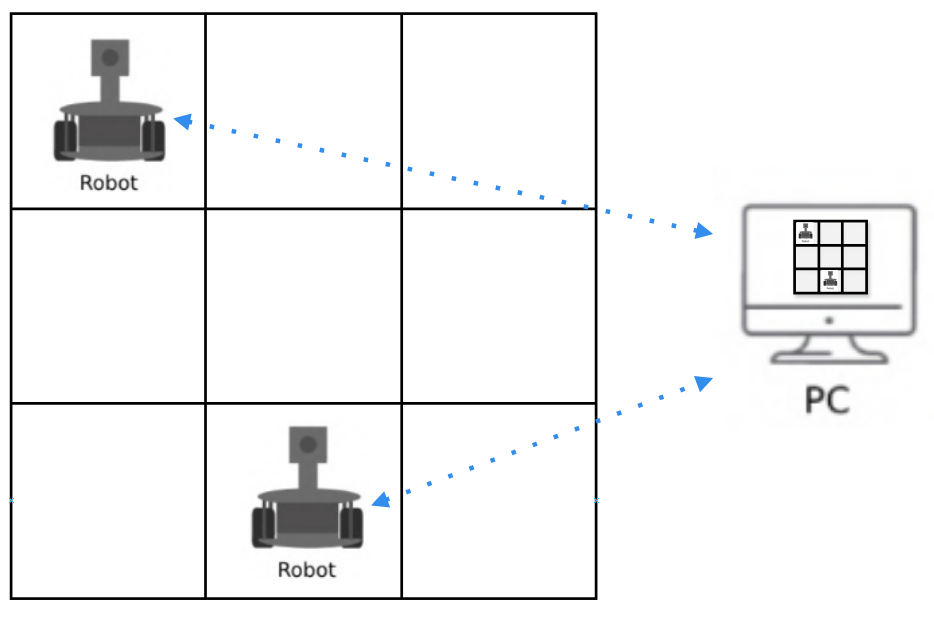
\includegraphics[width=0.65\linewidth]{mt_alto-nivel.png}
    \caption{Propuesta de alto nivel}
    \label{fig:propaltonivel}
\end{figure}


% fuentes de esta seccion
% https://www.sewio.net/uwb-technology/two-way-ranging/

\chapter{Marco teórico}

Todo proyecto robótico tiene por objeto crear un sistema complejo, cuyo desarrollo requiere conocimientos interdisciplinarios. El robot se coloca, de hecho, en la frontera entre la mecánica, la electrónica, el automóvil y la informática, lo que dentro de la industria 4.0 se denomina un sistema ciberfísico. Con todo esto podemos decir que nuestro robot debe contar con, al menos, las siguientes características:

\begin{itemize}
    \item Poseer 4 ruedas omnidireccionales controladas.
    \item Poder coexistir en el mismo espacio con otros robots.
    \item Determinar su posición en todo momento.
    \item Poder capturar imágenes con una cámara.
\end{itemize}

Se llevarán a cabo análisis de los puntos mencionados para conocer qué alternativas existen para abordar el proyecto y qué tópicos necesitamos conocer para llevar a cabo el desarrollo.

\section{Estado del arte}

La tecnología robótica se encuentra en plena fase de crecimiento, y por lo tanto, es previsible una presencia cada vez mayor de los robots, tanto en el sector industrial y de servicios, como en el sector doméstico. Como ha ocurrido en la informática, el desarrollo de robots se hace cada vez más accesible y por consiguiente sus capacidades tienden cada vez mayores gracias al aporte de una comunidad en auge. Este aumento en el interés de las personas sobre esta área, plantea ciertos desafíos, no solo en los aspectos tecnológicos, sino, también desde el punto de vista cultural y ético.

En la última mitad del siglo pasado el foco estaba puesto sobre todo en el campo de la robótica para impulsar el desarrollo de la producción a gran escala. Hoy se ha logrado gracias a ello un nivel tal de tecnología que el estudio y la realización de robots flexibles capaces de adaptarse a diferentes propósitos a diferentes entornos de trabajo ya no es una utopía. Desde el año dos mil, la investigación en el campo robótico también se dirige hacia el diseño de robots dedicados a la exploración del medio ambiente y de los llamados "robots de servicio".

Si hacemos foco en lo que respecta a los robots exploradores móviles, los mayores avances tecnológicos se dan en la exploración de otros planetas. Actualmente los científicos están enfocados en el planeta Marte así como lo fue en su momento la superficie Lunar. Los primeros desarrollos de este tipo de vehículos no tripulados surgen principalmente durante la carrera espacial entre USA y la URSS en la década del 60/70, donde los más conocidos, exceptuando los exploradores lunares han sido los siguientes:

Mars3 enviado en 1971 por la URSS el cual funcionó sobre la superficie marciana durante unos escasos 20 segundos.

\begin{figure}[H]
    \centering
    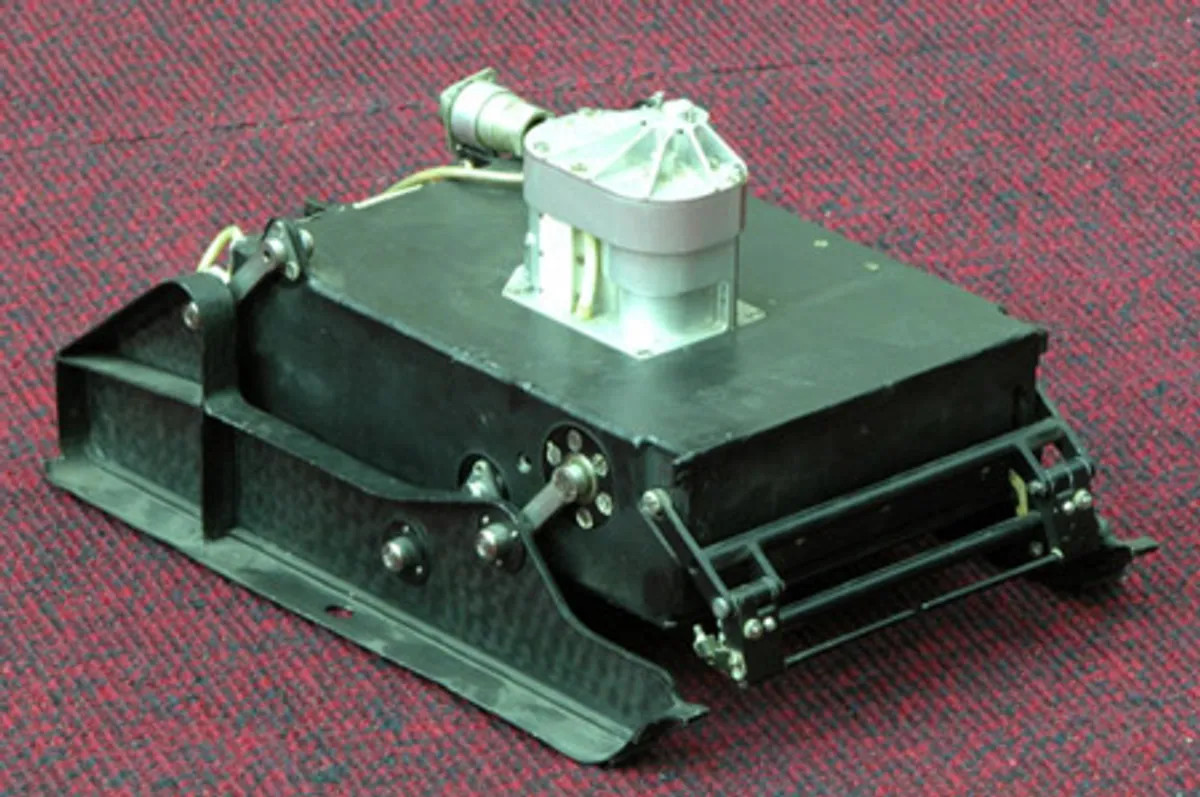
\includegraphics[width=0.5\linewidth]{images/mars3.jpg}
    \caption{Robot Mars3}
    \label{fig:mars3}
\end{figure}

En 2003, la NASA envió dos vehículos idénticos de 174 kilogramos con seis ruedas y paneles solares para recorrer parte de la superficie marciana, el Spirit y el Opportunity. El primero transmitió datos que hacen pensar que en el pasado existió agua líquida en Marte, hasta que se atasco y dejó de funcionar. El Opportunity todavía está operativo y ostenta el récord de distancia recorrida en otro planeta, con más de 42,6 kilómetros hasta el momento.

\begin{figure}[H]
    \centering
    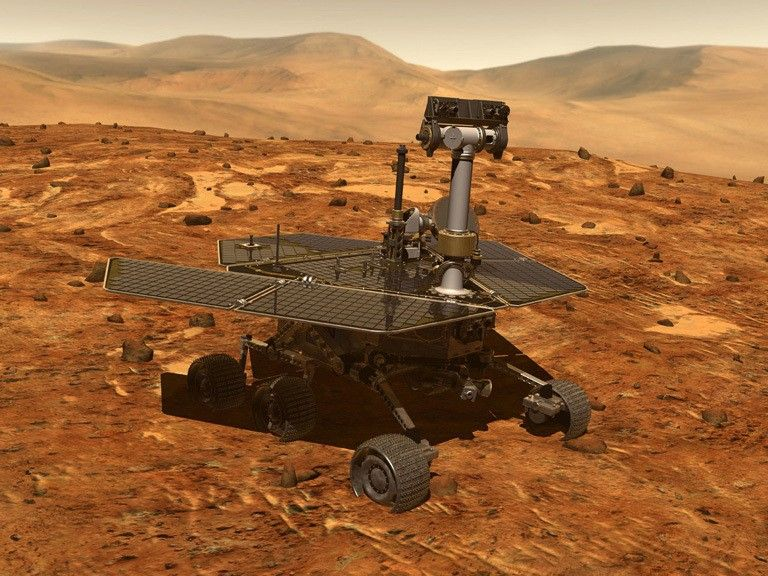
\includegraphics[width=0.5\linewidth]{images/opportunity-3d-model.jpg}
    \caption{Robot Opportunity}
    \label{fig:robot_opportunity}
\end{figure}

En 2011 la NASA envió a Marte el Curiosity, el vehículo más pesado (899 kilogramos) que nunca ha llegado a ese planeta. Aún está operativo y ha aportado las primeras evidencias de moléculas orgánicas en el planeta rojo.

\begin{figure}[H]
    \centering
    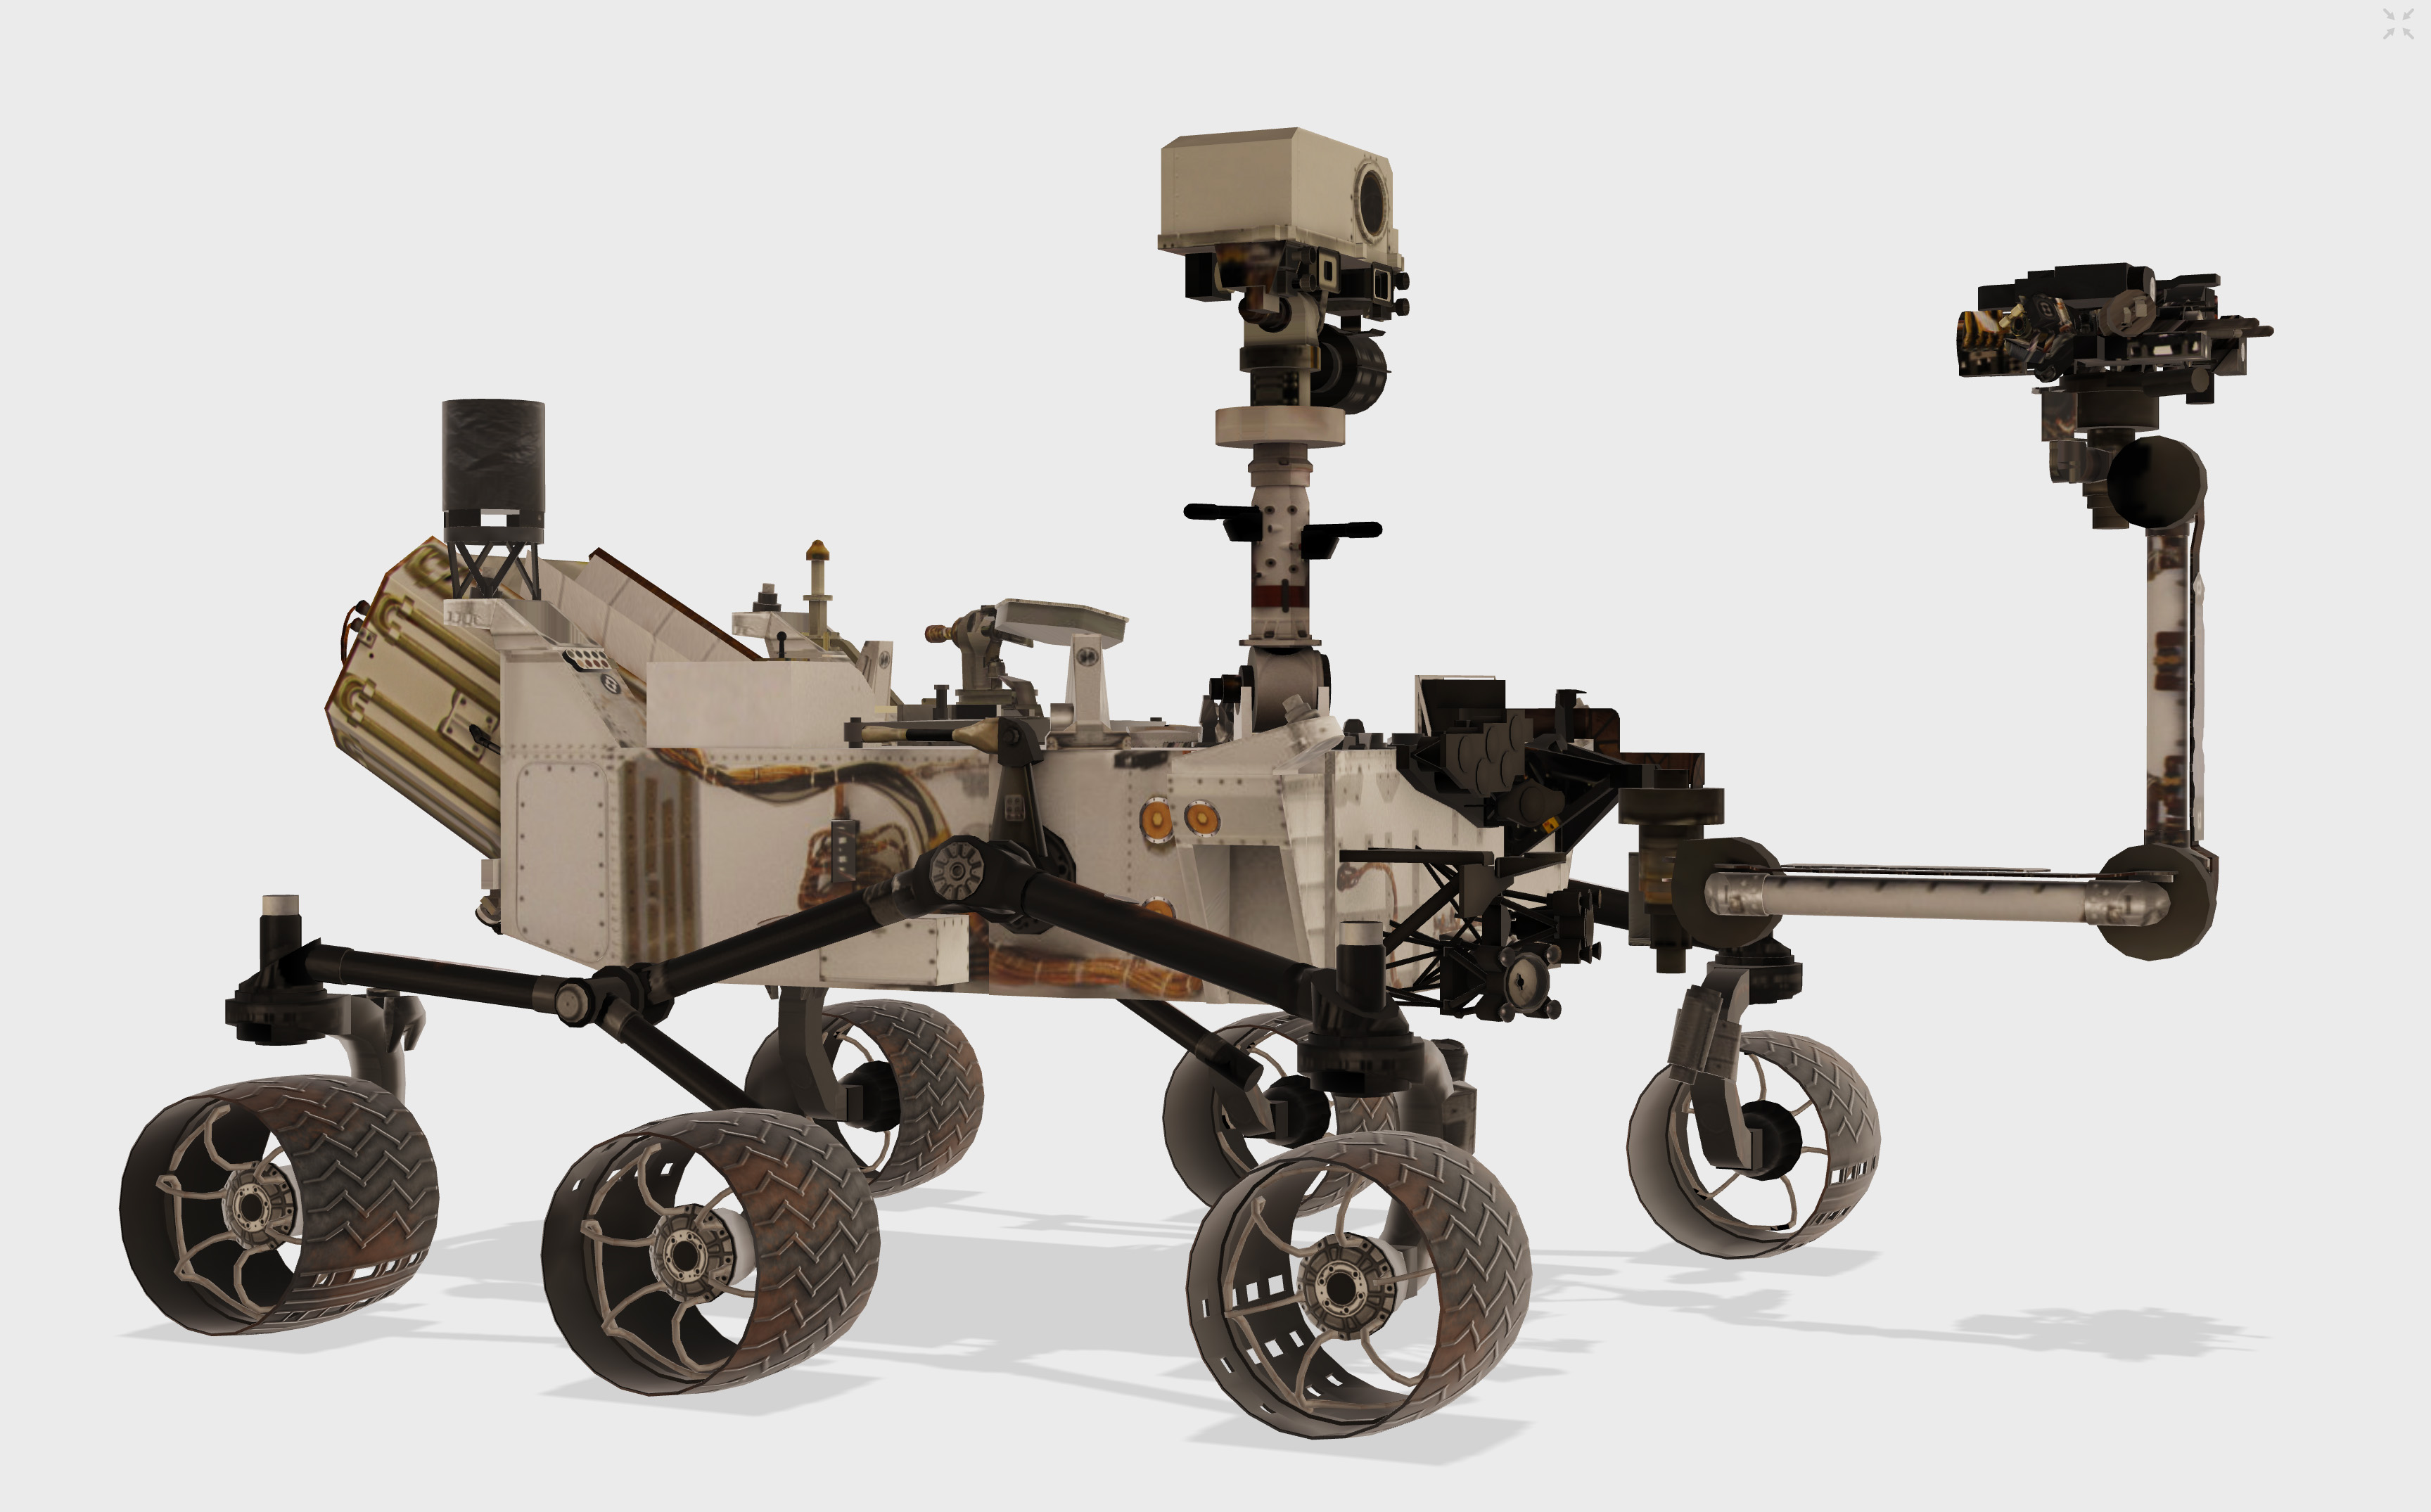
\includegraphics[width=0.5\linewidth]{images/curiosity-3d-model.jpg}
    \caption{Robot Curiosity}
    \label{fig:robot_curiosity}
\end{figure}

El 14 de marzo de 2016 la ESA y la Roscosmos enviaron a Marte la misión ExoMars, la primera de dos misiones que buscan analizar la atmósfera y colocar en su superficie dos vehículos, el segundo (2018) capaz de excavar dos metros por debajo de la superficie.

\begin{figure}[H]
    \centering
    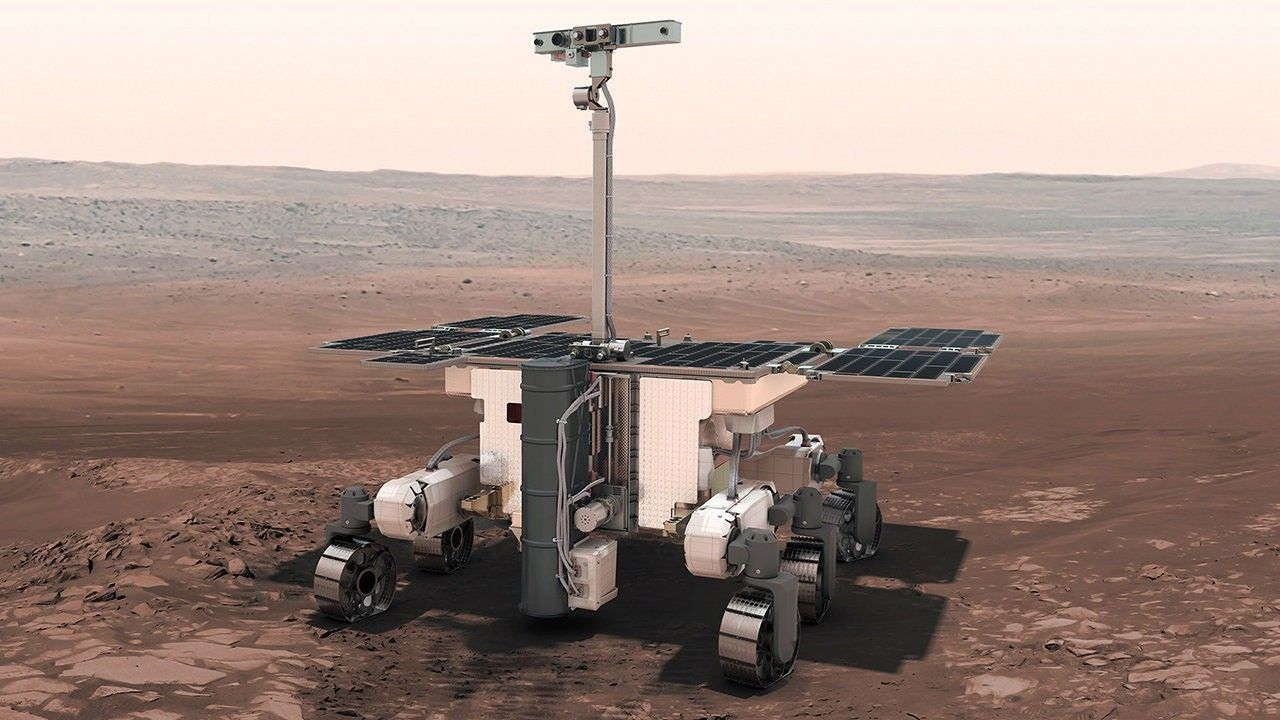
\includegraphics[width=0.5\linewidth]{images/Exomars_Rover.jpg}
    \caption{Robot ExoMars Rover}
    \label{fig:robot_exomarsrover}
\end{figure}

Por otra parte, tenemos a la robótica de servicio que es útil en el campo de la robótica médica, para la asistencia en rehabilitación y cirugía, así como en el campo doméstico para realizar tareas de limpieza y vigilancia.

La robótica móvil para estos sectores se ha convertido en una "herramienta de trabajo" importante y cada vez adquiere mayor protagonismo.

En los últimos años, mientras que la investigación de punta se enfoca en el diseño de robots para la exploración de Marte, en virtud de las tecnologías desarrolladas para tal fin, se hicieron los primeros robots para uso civil. Algunos de ellos, gracias a su pequeño tamaño y bajo costo de producción, gozan de cierto éxito comercial. Podemos mencionar de ejemplos al robot Roomba, hecho para la limpieza y lavado de pisos, una tarea que podría considerarse sencilla pero que implica un intenso trabajo computacional.

Sea cual sea el ámbito de aplicación, el diseño de robots móviles de pequeño tamaño y bajo costo de producción, pero, equipados con lógica de control avanzada, ha demostrado ser una gran utilidad para el hombre.

\section{Codiseño hardware-software}

El codiseño hardware-software es un enfoque metodológico que busca optimizar el rendimiento, la eficiencia y la funcionalidad de un sistema mediante la integración y colaboración estrecha entre el diseño del software y el hardware desde las etapas iniciales del desarrollo. En el contexto de un robot omnidireccional, la arquitectura de alto nivel debe ser cuidadosamente planificada para garantizar que ambos componentes trabajen de manera sinérgica, maximizando las capacidades del sistema y minimizando sus limitaciones. En nuestro caso se trata de un cyberphysical system dado que combina elementos de hardware, software y conectividad.

A continuación, se presentan las consideraciones clave y los tópicos más relevantes en el proceso de codiseño.

\subsection{Consideraciones clave}
El desarrollo de un sistema robótico eficiente y funcional requiere una definición clara y precisa de los requerimientos tanto funcionales como no funcionales. Al definirlos podemos encontrar aspectos como la precisión en la navegación, la capacidad de procesamiento en tiempo real, el consumo energético y la escalabilidad del diseño. Además, es esencial considerar las restricciones técnicas vinculadas al tamaño, el peso, el costo y la disponibilidad de los componentes, ya que estos factores tienen un impacto directo en las decisiones de diseño del sistema.

Un robot omnidireccional necesita realizar múltiples tareas de manera simultánea, como el procesamiento de datos sensoriales, la planificación de trayectorias y el control de los actuadores. Por ello resulta indispensable evaluar qué partes del sistema pueden ejecutarse de forma concurrente y distribuir las tareas entre el hardware y el software de modo eficiente.

La interacción entre el software y el hardware debe estar diseñada para garantizar una comunicación fluida y eficiente, minimizando los cuellos de botella que puedan limitar el rendimiento del sistema. Este aspecto incluye la selección adecuada de protocolos de comunicación, como SPI, I2C o Ethernet, así como la optimización del flujo de datos con el objetivo de reducir la latencia y mejorar la capacidad de respuesta general. \cite{lee2017introduction}

El uso equilibrado de los recursos hardware, como memoria, capacidad de cómputo y energía, con las demandas del software es otro factor esencial para optimizar el rendimiento del sistema. Se pueden implementar técnicas de optimización, como la compresión de datos o la reducción en la frecuencia de muestreo, siempre y cuando no se comprometa la funcionalidad del robot.

La arquitectura del sistema se diseña bajo principios de modularidad y escalabilidad, permitiendo la incorporación de nuevas funcionalidades o actualizaciones de componentes sin que se vea afectado el diseño global. Esta aproximación facilita la adaptabilidad del sistema a las necesidades futuras y contribuye a mitigar los costos asociados con la obsolescencia tecnológica.

Además, para garantizar la estabilidad y confiabilidad del sistema, es fundamental incorporar mecanismos de redundancia y recuperación ante fallos tanto en el hardware como en el software. La implementación de sistemas de monitoreo en tiempo real permite detectar errores de manera proactiva y corregirlos antes de que impacten la funcionalidad general del robot, asegurando así su robustez y tolerancia ante posibles fallos.


\subsection{Análisis de elementos necesarios}

Se analizan los elementos esenciales con los que debemos contar para así lograr la realización del proyecto. Estos elementos constituyen la base del proyecto, por lo que las decisiones tomadas al comienzo pueden repercutir en una etapa avanzada del mismo.


\subsubsection{Plataforma de hardware}

La selección de la plataforma hardware constituye un aspecto fundamental en el diseño de un sistema robótico, ya que debe equilibrar aspectos como la potencia de cálculo, el consumo energético y el costo. Entre las opciones disponibles, se encuentran los microcontroladores, como los basados en ARM Cortex u otros tales como Raspberry Pi, NVIDIA Jetson y las FPGAs. Están destinados a contener la lógica de control, monitoreo y comunicación inalámbrica. La plataforma elegida debe ser capaz de realizar operaciones en tiempo real.

También resulta crucial integrar componentes como sensores y actuadores que interactúen con el entorno. Los actuadores son los dispositivos encargados de interactuar con el medio en el que el robot se dispone y los sensores son los encargados de tomar muestras de magnitudes físicas de interés, como velocidad y distancia. \cite{lee2017introduction}

Dado que el robot debe operar con baterías y éstas son de capacidad limitada, la gestión de energía se convierte en un factor crítico. Optimizar el consumo energético requiere técnicas como el escalado dinámico de frecuencia o la hibernación de componentes no utilizados. También es recomendable incluir baterías de alta capacidad o sistemas de recarga automática para extender la autonomía del robot y mejorar su sostenibilidad operativa.


\subsubsection{Plataforma de software}
En cuanto a la arquitectura de procesamiento, es necesario definir si el diseño será centralizado, con un único procesador, o distribuido, utilizando múltiples procesadores o núcleos. Para sistemas complejos, como los robots omnidireccionales, una arquitectura distribuida suele ser preferible, ya que permite asignar tareas específicas a unidades de procesamiento dedicadas. Esta estrategia no solo optimiza el rendimiento del sistema, sino que también incrementa su eficiencia operativa en escenarios exigentes.

El desarrollo de software debe realizarse utilizando sistemas operativos en tiempo real o frameworks especializados, como ROS (Robot Operating System) o FreeRTOS, que permiten una gestión eficiente de tareas y recursos. A su vez, es fundamental implementar algoritmos optimizados para funciones clave como la navegación, la localización y el control, con el objetivo de garantizar un desempeño confiable en condiciones reales.

Debe señalarse además que son necesarios mecanismos lógicos de control para modelar todo el sistema junto con sus reglas. Para esto existen herramientas como Redes de Petri, que nos permiten modelar sistemas complejos con elementos sencillos.

Del mismo modo, la plataforma de software debe proveer al usuario de una interfaz interactiva donde pueda ejecutar órdenes y monitorear el estado de los robots en todo momento.


\subsubsection{Comunicación y sincronización}
El diseño de la comunicación y sincronización entre los distintos módulos del robot es esencial para garantizar un funcionamiento fluido y coordinado. Es indispensable implementar un sistema de comunicación eficiente que conecte sensores, actuadores y la unidad de control, además de mecanismos de sincronización que aseguren que las tareas se ejecuten en el orden y momento correctos, optimizando así el rendimiento global del sistema. \cite{lee2017introduction}

Al mismo tiempo, la latencia resulta crítica en aplicaciones robóticas. Una baja latencia asegura que el robot pueda reaccionar de manera inmediata a cambios en su entorno, como la aparición de obstáculos o la necesidad de ajustar su trayectoria. Esto es particularmente importante en entornos dinámicos, donde los retrasos en la toma de decisiones pueden resultar en colisiones o fallos en la navegación.


\subsubsection{Localización en tiempo real}

Para lograr que el robot navegue de modo autónomo, debemos utilizar los sensores y algoritmos avanzados de control, navegación y aprendizaje automático. Un sistema de cómputo potente permite implementar técnicas como el Filtro de Kalman para la estimación de la posición, algoritmos de planificación de rutas y sistemas de control predictivo, lo que mejora la precisión y eficiencia del robot. Todo esto permite la implementación de navegación autónoma, junto con la detección y evitación de obstáculos en tiempo real, además de integrar tareas de reconocimiento y aprendizaje.

Para justificar esto, debemos pensar que un robot omnidireccional dependerá de una gran cantidad de datos provenientes de sensores (cámaras, sensores de proximidad, giroscopios, etc.) para navegar y evitar obstáculos. Estos datos deben ser procesados en tiempo real para tomar decisiones rápidas y precisas, por lo cual un sistema de cómputo con alta capacidad de cálculo permite realizar operaciones complejas, como la fusión de datos sensoriales, la ejecución de algoritmos de localización y mapeo (SLAM, Simultaneous Localization and Mapping), y la planificación de trayectorias, de manera eficiente y sin retrasos. Esto implica la necesidad de procesamiento de datos en tiempo real. \cite{sariffpathplan}

En las subsiguientes secciones de este capítulo se profundiza sobre los distintos aspectos que nos son necesarios para la realización del proyecto.


\section{Movimiento y posicionamiento en interiores}

El control del movimiento y posicionamiento requiere procedimientos robustos que integren estrategias de planificación y ejecución en tiempo real.

Para que el robot se mueva por medio de sus ruedas, se utilizan controladores PID (Proporcional, Integral y Derivativo), los cuales ajustan dinámicamente las velocidades de las ruedas. Por otro lado, los sistemas más avanzados pueden integrar estrategias de Control Predictivo por Modelo (MPC), optimizando la trayectoria del robot mediante predicciones basadas en el modelo cinemático. Adicionalmente, el robot debe incorporar sensores para la retroalimentación del movimiento, como encoders en las ruedas y acelerómetros. Esta información es utilizada para ajustar y corregir el control en tiempo real.

Los algoritmos de control, como los basados en PID (Proporcional, Integral y Derivativo) o MPC (Control Predictivo por Modelo), permiten ajustar las velocidades y trayectorias del robot de manera precisa para evitar colisiones y garantizar estabilidad. Además, la navegación en interiores puede beneficiarse de técnicas como la SLAM (Simultaneous Localization and Mapping), que combina la localización con la construcción de mapas del entorno, ofreciendo una representación dinámica y actualizada. Cabe destacar la existencia de estimadores de estado genéricos como ser Filtro de Kalman, que permite la fusión de datos de múltiples sensores.

En la actualidad, los sistemas de posicionamiento en interiores (IPS, por sus siglas en inglés) se han convertido en una herramienta esencial en la navegación en espacios cerrados. La implementación de estas tecnologías puede lograrse mediante el uso de balizas de radiofrecuencia (Bluetooth, Wi-Fi, banda ultra ancha UWB), ultrasonido, etiquetas RFID y comunicaciones por luz visible (VLC, por sus siglas en inglés). \cite{nuaimisurveyindoorpositioning}

A pesar de los avances logrados, el posicionamiento asistido por GPS en interiores presenta limitaciones significativas debido a la gran pérdida de trayectoria provocada por las paredes de los edificios. Este debilitamiento de la señal lo convierte en una opción poco viable en comparación con otras tecnologías más especializadas.

Por otro lado, el uso de ultrasonido presenta problemas derivados de la alta atenuación en el aire, lo que dificulta su aplicación en eventos que requieran un amplio alcance. Otros métodos de posicionamiento, como infrarrojos, Zigbee y Bluetooth, aunque prometedores, pueden ser vulnerables a fluctuaciones en las fuentes de señal. No obstante, esta limitación podría mitigarse a través de soluciones como la implementación de una granja de antenas para garantizar una señal estable. En términos de precisión, las tecnologías tradicionales como Wi-Fi, Bluetooth y RFID activo proporcionan una precisión que generalmente varía en el rango de varios metros.

En cuanto a las comunicaciones de luz visible (VLC), se destacan por su enfoque innovador al detectar luz mediante fotodetectores. El uso de un único detector permite realizar una lateralización circular, mientras que la implementación de dos detectores habilita un posicionamiento diferencial. Este último método ha demostrado un mejor desempeño y una mayor reducción en el margen de error, consolidándose como una solución prometedora para futuros desarrollos tecnológicos en el ámbito del posicionamiento en interiores.

Cambien podemos mencionar los seguidores de línea, que representan un ejemplo simplificado de navegación basada en detección. Se emplean sensores para identificar y seguir líneas o patrones, que actúan como guías para el control del movimiento y la localización en entornos estructurados.

A continuación se detalla una tabla comparativa sobre las diferentes alternativas para posicionamiento en interiores, entre ellos, los distintos sistemas de localización en tiempo real que existen, también conocidos como RTLS \cite{alammarsurveyindoor}.

\begin{figure}[H]
    \centering
    \hspace*{-1.0cm}
    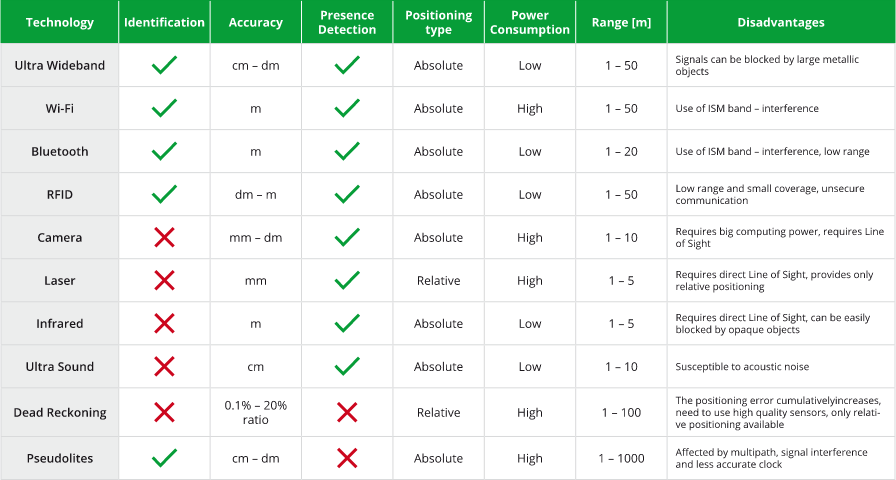
\includegraphics[width=1.1\linewidth]{mt_RTLS_comparacion}
    \caption{Tabla comparativa entre métodos de posicionamiento en interiores extraída de \textit{sewio.net} \cite{sewiortls}}
    \label{fig:compmetposindor}
\end{figure}


\subsection{Filtro de Kalman}

El filtro de Kalman constituye una herramienta esencial en la robótica para la estimación del estado de un sistema dinámico en entornos sujetos a incertidumbre y ruido en las mediciones. En el caso de robots omnidireccionales, su aplicación es particularmente útil para determinar la posición de un objeto en tiempo real mediante la integración de datos provenientes de múltiples sensores. Este proceso permite superar las limitaciones impuestas por el ruido inherente y las diferencias en las frecuencias de muestreo de los sensores.

El funcionamiento del filtro de Kalman se fundamenta en dos etapas principales: la predicción y la actualización. En la fase de predicción, se estima el estado del sistema y su incertidumbre utilizando modelos cinemáticos que describen el movimiento del objeto. En la etapa de actualización, las observaciones obtenidas de los sensores se incorporan para ajustar la estimación, ponderando cada medición según su nivel de precisión. Este enfoque posibilita la integración eficaz de entradas provenientes de sensores como cámaras, acelerómetros, encoders, entre otros, incluso cuando las frecuencias de muestreo difieren entre sí. \cite{nuaimisurveyindoorpositioning}


\subsection{Detección y medición de QR}

La detección y utilización de códigos QR en la robótica interior han demostrado ser una solución económica y eficiente para la navegación y localización del robot. Estos códigos, colocados en paredes y áreas visibles, pueden almacenar información relevante sobre el entorno, como la sección o ubicación específica dentro del espacio. Además, su bajo costo de producción los hace ideales para proyectos de robótica en interiores. \cite{tzafestas2013introduction}

La lectura de los códigos QR se realiza mediante cámaras integradas en el robot. Estas cámaras capturan imágenes del código y, utilizando técnicas de procesamiento de imagen, decodifican la información almacenada. Además, se puede estimar la distancia entre el robot y el código QR con un nivel razonable de precisión, aprovechando el tamaño conocido del código y las características del encuadre de la cámara. Este cálculo, basado en principios de geometría proyectiva, permite al robot ajustar su posición y orientar sus movimientos en función de los datos obtenidos.


\section{Redes de Petri}

Una red de Petri es un modelo gráfico, formal y abstraco para la representación de sistemas distribuidos y el análisis del flujo de información. Este modelo facilita la comprensión sobre la estructura y el comportamiento dinámico y estático del sistema modelado. Las redes de Petri son de utilidad principalmente en el diseño de sistemas de hardware y software para especificación, simulación y diseño de diversos problemas de ingeniería, especialmente útiles para representar procesos concurrentes, asó como procesos donde puedan existir restricciones en cuanto a la simultaneidad, la precedencia o la frecuencia de eventos concurrentes.\\

Las redes de Petri están fuertemente asociadas a la teoría de grafos, ya que las mismas pueden representarse como un grafo dirigido bipartito compuesto por cuatro elementos:

\begin{itemize}
    \item Plazas: representan los estados del sistema. Estas son variables de estado que pueden tomar valores enteros.
    \item Tokens: figuran como puntos dentro de las plazas. Estos representan el valor específico de una condición o estado y generalmente se traducen a la presencia o ausencia de algún recurso del sistema.
    \item Transiciones: representan el conjunto de sucesos cuya ocurrencia produce la modificación de los estados (y en consecuencia del estado global) del sistema.
    \item Arcos: indican las interconexiones entre las plazas y las transiciones, estableciendo el flujo de tokens que sgieu el sentida de la flecha.
\end{itemize}

Una vez definidos sus componentes, se puede decir que una red de Petri es un grafo dirigido con dos tipos de nodos: plazas y transiciones. Estos nodos están vinculados por arcos, los cuales sólo puede conectar una plaza con una transición o viceversa. Por otro lado, una red de Petri puede ser descrita mediante dos componentes:

\begin{enumerate}
    \item Una estructura de red
    \item Un marcado inicial
\end{enumerate}

La estructura de red hace referencia a la red en sí, mientras que el marcador inicial sólo representa el estado inicial del sistema (denominado estado idle), es decir, sin que ninguna transición haya sido disparada. Un ejemplo simple de una red de Petri marcada se muestra en la Figura \ref{fig:rdp_marcada}. Este será utilizado en las secciones siguientes para ilustrar operaciones y/o propiedades de las redes de Petri.

\begin{figure}[H]
    \centering
    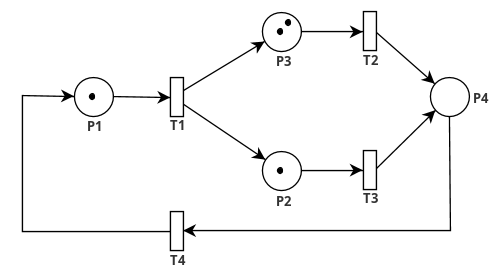
\includegraphics[width=0.6\linewidth]{images/rdp_marcada.png}
    \caption{Red de Petri marcada}
    \label{fig:rdp_marcada}
\end{figure}

\subsection{Estructura de una red de Petri ordinaria}
La estructura de una red de Petri puede definirse como una tupla de 5 elementos (5-tupla) de la siguiente manera:

\begin{equation}
    N = (P, T, I^-, I^+, M_0)
\end{equation}

Donde:
\begin{itemize}
    \item $P = \{P_1, P_2, ..., P_n\}$ es un conjunto finito y no vacío que contiene todas las plazas de la red.
    \item $T = \{T_1, T_2, ..., T_n\}$ es un conjunto finito y no vacío que contiene todas las transiciones.
    \item $I^-$ y $I^+$ son las matrcices pre y post respectivamente, cuya composición se abordará en la próxima sección.
    \item $M_0$ es el marcado inicial de la red. Definido como un vector con un elemento para cada plaza, donde $M_0[i]$ contendrá la cantidad de tokens en la plaza $i$ para el estado inicial.
\end{itemize}

Siguiendo con el ejemplo propuesto en la sección anterior \ref{fig:rdp_marcada}, se puede representar la red como $N = (P, T, I^-, I^+, M_0)$ donde:

\begin{itemize}
    \item $P = \{P_1, P_2, P_3, P_4\}$
    \item $T = \{T_1, T_2, T_3, T_4\}$
    \item $M_0 = [1, 1, 2, 0]$
\end{itemize}

A continuación se explicará la manera de obtener las matrices $I^-$ e $I^+$.

\subsection{Matriz de incidencia}
Las matrices $I^-$ e $I^+$ son las funciones de incidencia de entrada y salida de las plazas. Para el caso de la matriz $I^+$, denominada post, se tiene que cada elemento $post(P_i, T_j)$ contiene el peso asociado al arco que va desde $T_j$ hasta $P_i$. Este peso indica la cantidad de tokens que se generan en la plaza $P_i$ cuando la transición $T_j$ es disparada.\\

Por otro lado, en la matriz $I^-$, denominada pre, cada elemento $pre(P_i, T_j)$ contiene el peso asociado al arco que va desde $P_i$ hasta $T_j$ indica la cantidad de tokens que se retiran de la plaza $P_i$ cuando se dispara la transición $T_j$.\\

Siguiendo con el ejemplo de la Figura \ref{fig:rdp_marcada}, las matrices $I^-$ e $I^+$ asociadas son:
\begin{equation}
I^+ =
    \begin{pmatrix}
        0 & 0 & 0 & 1\\
        1 & 0 & 0 & 0\\
        1 & 0 & 0 & 0\\
        0 & 1 & 1 & 0
    \end{pmatrix}
\end{equation}
    
\begin{equation}
I^- =
    \begin{pmatrix}
        1 & 0 & 0 & 0\\
        0 & 1 & 0 & 0\\
        0 & 0 & 1 & 0\\
        0 & 0 & 0 & 1
    \end{pmatrix}
\end{equation}

Las filas de las matrices representan las plazas mientras que las columnas representan las transiciones, lo cual quiere decir que las matrices tendrán tantas filas como plazas tenga la red de Petri, y tantas columnas como transiciones.\\

De esta forma se puede observar como el elemento $I^-[0][0]$ indica la relación de salida entre $P_1$ y $T_1$. Más precisamente indica que cuando $T_1$ se dispara, solo un token es retirado de $P_1$ (ya que el peso del arco entre $P_1$ y $T_1$ es 1). De igual manera, el elemento $I^+[0][0] = 0$ indica que cuando la misma transición se dispara, no se genera ningún token en $P_1$ (ya que no existe ningún arco que parta de $T_1$ hacia $P_1$).\\

A partir de estas definiciones, se puede obtener la matriz de incidencia de la red. La misma está definida a continuación:\\

\begin{equation} I = I^+ -\ I^- \end{equation}

Cabe aclarar que una red de Petri puede reconstruirse completamente a partir de sus matrices $I^-$ e $I^+$, pero no así si se tiene sólo la matriz de incidencia $I$. Esto quiere decir que puede haber varias redes de Petri distintas con la misma matriz de incidencia, pero solamente una para las matrices $I^-$ e $I^+$. Sin embargo, cuando una red de Petri no tiene autobucles (presente cuando se tienen dos arcos con sentidos contrarios entre una misma plaza y transición), su matriz de incidencia determina completamente su estructura.\\

La matriz de incidencia asociada a la red de Petri de la Figura \ref{fig:rdp_marcada} será entonces:

\begin{equation}
I =
    \begin{pmatrix}
        0 & 0 & 0 & 1\\
        1 & 0 & 0 & 0\\
        1 & 0 & 0 & 0\\
        0 & 1 & 1 & 0
    \end{pmatrix}
-\ 
    \begin{pmatrix}
        1 & 0 & 0 & 0\\
        0 & 1 & 0 & 0\\
        0 & 0 & 1 & 0\\
        0 & 0 & 0 & 1
    \end{pmatrix}
=\ 
    \begin{pmatrix}
        -1 & 0 & 0 & 1\\
        1 & -1 & 0 & 0\\
        1 & 0 & -1 & 0\\
        0 & 1 & 1 & -1
    \end{pmatrix}
\end{equation}

\section{Dinámica de una red de Petri}
Se dice que una transición está sensibilizada cuando el marcado de todas las plazas entrantes a la transición es mayor o igual al peso de los arcos que las unen con dicha transición.\\

Antes de expresar la condición de sensibilizado de manera general, es necesario definir los siguientes conjuntos funciones:

\begin{itemize}
    \item $\bullet T_j$ es el conjunto compuesto por las plazas entrantes a $T_j$.
    \item $T_j \bullet$  es el conjunto compuesto por las plazas salientes de $T_j$.
    \item $\bullet \bullet P_i$ es el conjunto compuesto por las transiciones entrantes a las plazas que sensibilizan a las transiciones que le agregan tokens a $P_i$.
    \item $P_i \bullet \bullet$  es el conjunto compuesto por las transiciones entrantes a las plazas que sensibilizan a las transiciones que le quitan tokens a $P_i$.
    \item $m_k(P_i)$ es el marcado de la plaza Pi antes de disparar la transición $T_j$ .
    \item $m_{k+1}(P_i)$ es el marcado de la plaza $P_i$ después de disparar la transición $T_j$.
    \item $w_{ij}$ es el peso del arco $P_i \rightarrow T_j$.
    \item $w_{ji}$ es el peso del arco $T_j \rightarrow P_i$.
\end{itemize}

Entonces, el sensibilizado de una transición Tj está dado por:

\begin{equation}
    T_j \ est\acute{a} \ sensibilizada \ si \ \forall \ P_i \ \in \ \bullet T_j \Rightarrow m_k (P_i) > w_{ij}
\end{equation}

Esta definición de sensibilizado es solo válida cuando los arcos que conectan las plazas con $T_j$ son arcos comunes. \\
En la figura \ref{fig:rdp_sensibilizada} se resaltan las transiciones sensibilizadas del ejemplo anterior.

\begin{itemize}
    \item $T_1$, $T_2$, $T_3$ están sensibilizadas, mientras $T_4$ no está sensibilizada (ya que el marcado de $P_4$ es menor al peso del arco $P_4 \rightarrow T_4$ ).
\end{itemize}

\begin{figure}[H]
    \centering
    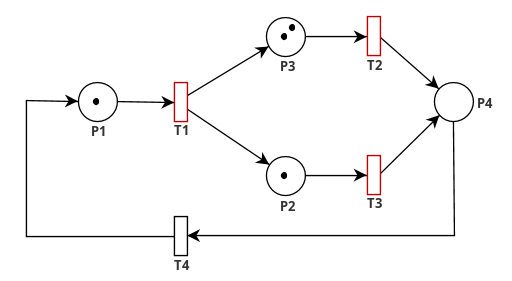
\includegraphics[width=0.6\linewidth]{images/rdp_sensibilizada.png}
    \caption{Transiciones sensibilizadas de la red de Petri}
    \label{fig:rdp_sensibilizada}
\end{figure}

\subsection{Disparo de una transición}
Si una transición está sensibilizada, la misma puede dispararse. El disparo de una transición resulta en un nuevo marcado de la red. Más precisamente, al ejecutarse una transición $T_j$ con un marcado $m_k$, los marcados de las plazas pertenecientes a la red se alteran cumpliendo con las siguientes declaraciones:

\begin{equation}
    \sigma (m_k, T_j) = 
    \begin{array}{cc}
         \forall \ P_i \ \in \ \bullet T_j \ \Rightarrow \ m_{k+1}(P_i) = m_k(P_i) - w_{ij}  \\
         \forall \ P_i \ \in \ T_j \bullet \ \Rightarrow \ m_{k+1}(P_i) = m_k(P_i) + w_{ji}  \\
         \forall \ P_i \ \notin \ \bullet T_j \cup T_j \bullet \ \Rightarrow m_{k+1}(P_i) = \ m_k(P_i)
    \end{array}
\end{equation}

\noindent Es decir:
\begin{itemize}
    \item Para todas las plazas entrantes a $T_j$, el nuevo marcado de cada plaza se habrá \textbf{decrementado} tantos $tokens$ como peso tenga el arco $P_i \rightarrow T_j$. 
    \item Para todas las plazas salientes de $T_j$, el nuevo marcado de cada plaza se habrá \textbf{incrementado} tantos $tokens$ como peso tenga el arco $T_j \rightarrow P_i$.
    \item Para el resto de las plazas, el nuevo marcado será exactamente igual al que tenían antes del disparo de $T_j$ .
\end{itemize}

Continuando con el ejemplo anterior, se puede observar en la figura \ref{fig:rdp_marcado_nuevo} el nuevo marcado de la red luego del disparo de la transición $T_3$:

\begin{itemize}
    \item La única plaza entrante a $T_3(P_3 )$, ha \textbf{decrementado} su marcado en 1 $token$ (ya que el peso del arco $P_3 \rightarrow T_3$ es 1).
    \item La plaza saliente de $T_j(P_4)$ ha \textbf{incrementado} su marcado de acuerdo a los pesos de los arcos correspondientes, en este caso en 1.
    \item Las plazas que no es entrante ni saliente de $T_3(P_3)$ ha mantenido su marcado original.
\end{itemize}

Cabe destacar que como consecuencia del disparo de $T_3$, se ha producido la sensibilización de $T_4$.

\begin{figure}[H]
    \centering
    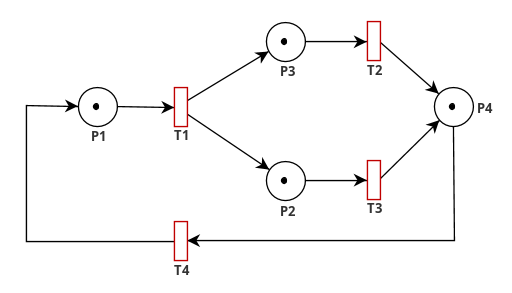
\includegraphics[width=0.6\linewidth]{images/rdp_marcado_nuevo.png}
    \caption{Nuevo marcado de la red de Petri}
    \label{fig:rdp_marcado_nuevo}
\end{figure}

\subsection{Función de transferencia y ecuación de estado}
Una vez explicada la dinámica del disparo de una transición y la forma de obtener la matriz de incidencia, se detalla una expresión matemática necesaria para obtener el nuevo marcado luego del disparo de una transición. 
La misma se denomina \textbf{función de transferencia} y está definida como el producto de la matriz de incidencia $I$ con un vector $\vec{\delta}$ cuyos componentes son todos ceros, exceptuando el componente asociado a la transición que se quiere disparar, cuyo valor será uno. Entonces, se tendrá:

\begin{equation}
    I \ . \ \vec{\delta }
\end{equation}

\noindent donde, para el disparo de una transición $T_j$ , se tiene:
\begin{itemize}
    \item $\delta[j] = 1$
    \item $\delta[i] = 0 \ \forall \ i/i \neq j$
\end{itemize}

Por otro lado, es necesario introducir la \textbf{ecuación de estado} de las redes de Petri. Con esta ecuación es posible obtener el siguiente estado del sistema luego del disparo de una transición. Esta es una manera más simple que la metodología gráfica para analizar la evolución de los sistemas. La ecuación de estado en un tiempo $i$, para calcular el nuevo marcado de la red en un tiempo $i+1$ se define como:

\begin{equation}
    M_{i+1} = M_i + I \ . \ \vec{\delta}
    \label{ec:estado}
\end{equation}

\noindent donde $M_{i+1}$ es el marcado luego del disparo de la transición, $M_i$ es el marcado antes del disparo y el segundo término de la ecuación es la función de transferencia.

Siguiendo con el ejemplo hasta ahora analizado se verá cómo calcular el marcado de la red luego del disparo de la transición $T_3$ haciendo uso de la ecuación de estado.

En la figura \ref{fig:rdp_sensibilizada} se observan las transiciones sensibilizadas de la red para el marcado inicial $M_0$.
\\
La ecuación de estado requiere tres elementos:
\begin{enumerate}
    \item El marcado antes del disparo. Éste es:
        \begin{equation}
            M_i = M_0 = 
            \begin{pmatrix}
                1 \\
                1 \\
                2 \\
                0
            \end{pmatrix}
        \end{equation}
        
    \item La matriz de incidencia de la red es la siguiente:
        \begin{equation}
           I = 
            \begin{pmatrix}
                -1 & 0 & 0 & 1 \\
                1 & -1 & 0 & 0 \\
                1 & 0 & -1 & 0 \\
                0 & 1 & 1 & -1 
            \end{pmatrix}
        \end{equation}
        
    \item El vector de disparo $\vec{\delta}$, que tendrá tantos elementos como transiciones haya en la red, cuyos valores serán cero para todas las transiciones excepto para aquella que se desee dispara:
        \begin{equation}
            \vec{\delta} = 
            \begin{pmatrix}
                0 \\
                0 \\
                1 \\
                0
            \end{pmatrix}
        \end{equation}
\end{enumerate}

\noindent con lo cual el nuevo marcado está definido por:
\begin{equation}
    M_{i+1} = 
    \begin{pmatrix}
        1 \\
        1 \\
        2 \\
        0
    \end{pmatrix}
    +
    \begin{pmatrix}
        -1 & 0 & 0 & 1 \\
        1 & -1 & 0 & 0 \\
        1 & 0 & -1 & 0 \\
        0 & 1 & 1 & -1 
    \end{pmatrix}
    .
    \begin{pmatrix}
        0 \\
        0 \\
        1 \\
        0
    \end{pmatrix}
    =
    \begin{pmatrix}
        1 \\
        1 \\
        1 \\
        1
    \end{pmatrix}    
\end{equation}

\noindent resultado que coincide con lo obtenido en la figura \ref{fig:rdp_marcado_nuevo}. La ecuación de estado representa matemáticamente el comportamiento dinámico del sistema, permitiendo calcular el nuevo estado del mismo luego de la ocurrencia de un evento a través de una simple ecuación.

\subsection{Extensión de la ecuación de estado}
Como se mencionó en la sección anterior, la ecuación \ref{ec:estado} permite calcular el siguiente estado luego del disparo de una transición. Sin embargo, puede que se desee obtener el marcado final luego de una secuencia de disparos. Suponiendo que se parte del estado inicial $M_0$, esto puede representarse como:

\begin{equation}
    M_i = M_0 + I \ . \sum_{j=1}^i u_j
\end{equation}

\noindent donde la sumatoria representa un vector asociado a la secuencia de transiciones que se desea disparar y se denomina vector S. Para ejemplificar, el cálculo de un marcado $M_i$ a partir del marcado inicial y luego del disparo de las transiciones {$T_3$, $T_4$, $T_1$, $T_2$,} está dado por:

\begin{equation}
    M_i = M_0 + I \ . \ \vec{S}
\end{equation}

\noindent donde $\vec{S}$ = \{ 1, 1, 1, 1 \} e $I$ es la matriz de incidencia asociada a la red.

\section{Propiedades de las redes de Petri}
\subsection{Propiedades de limitación}
Dada una red de Petri definida por $PN = \{ P, T, I^-, I^+, M_0 \}$, se dice que una plaza P está k-limitada si existe un número entero k que, para todo marcado posible de la red, se verifica que la cantidad de tokens de la plaza siempre es igual o menor a k. Es decir:

\begin{equation}
    \exists \ k \ \in \ N \ / \ \forall \ M \ \in \ marcados (PN) \Rightarrow M(P) \leq k
\end{equation}

\noindent Por otro lado, se dice que la red está \textbf{k-limitada} si todas las plazas que contiene son \textbf{k-limitadas}. \\ \par

A partir de la definición de limitación surgen varios conceptos, entre los cuales se encuentran los siguientes:
\begin{itemize}
    \item Una red de Petri es \textbf{segura} si todas sus plazas son \textbf{1-limitadas}. Esto significa que nunca puede darse un disparo si la plaza de llegada ya contiene un $token$.
    \item Una red de Petri es \textbf{cíclica} si siempre existe la posibilidad de alcanzar el marcado inicial desde cualquier otro marcado alcanzable. Es decir, \break $\forall \ M  \in \ marcados(PN),\ M_0$ es dinámicamente alcanzable desde $M$.
    \item Una red de Petri es \textbf{repetitiva} si existe una secuencia de disparos $\sigma$ que contiene todas las transiciones de la red y existe un marcado $M$ que para el cual $M \xrightarrow{\sigma} M$. Es decir, existe una secuencia de disparos que contiene todas las transiciones y que lleva la red del marcado actual al mismo marcado.
    \item  Una red de Petri es \textbf{conservativa} si se cumple que $\forall \ M\ \in marcados (PN)$, el número total de $tokens$ en el marcado M es igual al número de tokens en el marcado $M_0$. En otras palabras, la red siempre contiene la misma cantidad de marcas.
    
\end{itemize}

\subsection{Propiedades de vivacidad}
La \textbf{vivacidad} de una transición indica que, en todo instante de la  evolución de la red, su disparo es posible. Este concepto es particularmente relevante ya que determina si la ejecución de la red puede  o no detenerse en un estado determinado. A partir de esto se puede definir la vivacidad de una red de Petri. Esta propiedad indica que una red $N = \{P, T, I^- , I^+ , M_0 \}$ es viva para un marcado si todas sus transiciones lo son.

Por otro lado, la \textbf{cuasi-vivacidad} de una transición expresa la posibilidad de dispararla al menos una vez a partir de un marcado inicial $M_0$. De la misma manera que para el caso de la vivacidad, una red de Petri es cuasi-viva si todas sus transiciones lo son.

Gracias a esta última definición, se puede definir la vivacidad en función de la cuasi-vivacidad de la siguiente manera: una transición es viva si la misma es cuasi-viva en la red para todo marcado alcanzable desde $M_0$. \\ \par

\noindent La vivacidad está directamente asociada con la ausencia de \textbf{deadlock} o interbloqueo. En términos generales, el deadlock es el bloqueo permanente de un conjunto de procesos o hilos de ejecución en un sistema concurrente que compiten por recursos del sistema o bien se comunican entre ellos. En el caso de una red de Petri, esto suele ocurrir cuando dos o más transiciones esperan mutuamente por el disparo de la otra, produciendo el bloqueo permanente de esa porción de la red. 
Una red de Petri viva garantiza la ausencia de interbloqueo sin importar la secuencia de disparos.

\subsection{Alcanzabilidad de una red de Petri}
La \textbf{alcanzabilidad} de una red de Petri es fundamental para el análisis de las propiedades dinámicas de un sistema. A grandes rasgos, permite determinar si el sistema modelado puede alcanzar un determinado estado.

Un marcado $M_i$ es alcanzable desde $M_0$ si existe una secuencia finita de disparos $\sigma$ tal que $M_0 \xrightarrow{\sigma} M_i$.

Los marcados alcanzables por la red pueden ser representados como nodos de un grafo o árbol, donde los arcos indican los disparos necesarios para alcanzar dicho marcado. El algoritmo para determinar el árbol de alcanzabilidad de una red de Petri será explicado con detalle en el desarrollo del proyecto.

Entonces, el grafo de alcanzabilidad $A$ se define como el menor conjunto que cumpla con las expresiones \ref{ec:marcado_inicial} y \ref{ec:marcado_alcanzable}.

\begin{equation}
    M_0 \ \in \ A
    \label{ec:marcado_inicial}
\end{equation}

\noindent Esta condición simplemente aclara que el marcado inicial de la red siempre forma parte del grafo de alcanzabilidad, ya que el mismo no requiere ninguna secuencia de disparos para ser alcanzable.

\begin{equation}
    \forall \ M \ sii \ M \xrightarrow{\sigma} M_i \Rightarrow M_i \ \in \ A
    \label{ec:marcado_alcanzable}
\end{equation}

\noindent Esto significa que para cualquier marcado $M$, si a partir del mismo puede alcanzarse otro marcado $M_i$, entonces $M_i$ forma parte del grafo. \\ \par

\noindent Suponiendo una red simple como la de la figura \ref{fig:rdp_3_estados}, compuesta por tres plazas y una única transición $T_1$ , se puede afirmar que sólo hay tres estados posibles en la red:

\begin{figure}[H]
    \centering
    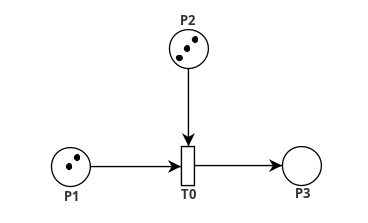
\includegraphics[width=0.5\linewidth]{images/rdp_3_estados.png}
    \caption{Red de Petri 3 estados posibles}
    \label{fig:rdp_3_estados}
\end{figure}

\begin{itemize}
    \item El marcado inicial [2, 3, 0]
\end{itemize}

Luego del segundo disparo no existen disparos posibles. Por lo tanto, la red de la figura \ref{fig:rdp_3_estados} produce el grafo de alcanzabilidad mostrado en la figura \ref{fig:grafo_alcanzabilidad}. \\

\begin{figure}[H]
    \centering
    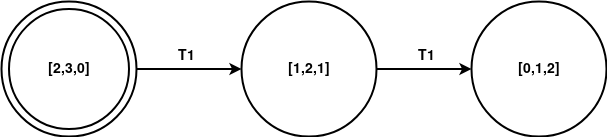
\includegraphics[scale=0.4]{images/grafo_alcanzabilidad.png}
    \caption{Grafo de alcanzabilidad.}
    \label{fig:grafo_alcanzabilidad}
\end{figure}

\subsection{Sifones y Trampas}
Los conceptos de sifón y trampa están directamente relacionados con las propiedades de \textbf{interbloqueo} y \textbf{vivacidad} de una red de Petri.

Un \textbf{sifón} se define como un subconjunto no vacío de plazas S para el cual se cumple que el subconjunto de transiciones entrantes a S está contenido dentro del subconjunto de transiciones salientes de S.
En otras palabras, un grupo de plazas es un sifón si, una vez que un token sale del grupo de dichas plazas, el mismo nunca puede volver a entrar. 
Decimos que un sifón S es \textbf{mínimo} si no contiene otro sifón como un subconjunto. En un sifón mínimo debe existir al menos dos lugares; de lo contrario, la estructura restante no puede considerarse un sifón.
En la figura \ref{fig:rdp_sifon_trampa} se puede observar una red que contiene una trampa y un sifón.

\begin{figure}[H]
    \centering
    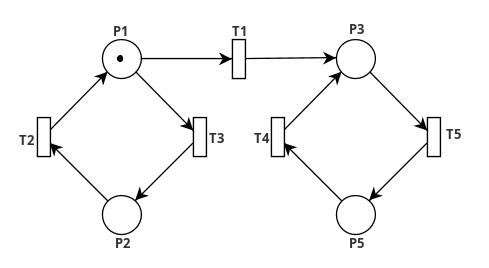
\includegraphics[width=0.8\linewidth]{images/rdp_sifon_trampa.png}
    \caption{Sifón y trampa}
    \label{fig:rdp_sifon_trampa}
\end{figure}

Tomando el subconjunto de plazas $S = \{P_1 , P_2 \}$ se deben obtener los siguientes subconjuntos de transiciones:
\begin{itemize}
    \item El subconjunto $\bullet S = \{T_2, T_3 \}$ será aquel compuesto por las transiciones entrantes a las plazas que componen S.
    \item El subconjunto $S \bullet = \{T_2, T_3\} $ será aquel compuesto por las transiciones entrantes a las plazas que componen S.
\end{itemize}

\noindent Por propiedad de los sifones, para que S pueda considerarse como tal debe cumplirse que:
\begin{equation}
    \bullet S \ \subseteq \ S \bullet 
\end{equation}

En este caso, se comprueba que ${T_2 , T_3} \subseteq \ \{T_1 , T_2 , T_3 \}$, quedando demostrado que $\{P_1,P_2\}$ es en efecto un sifón y que, si la transición $T_1$ se dispara, el token removido de $P_1$ nunca volverá a ingresar al subconjunto. \\ \par

Por otro lado, una \textbf{trampa} se define como un subconjunto de plazas G para el cual se cumple que el subconjunto de transiciones salientes de G está contenido dentro del subconjunto de transiciones entrantes a G. Esto quiere decir que un conjunto de plazas constituyen una trampa si una vez que un token entra dicho grupo éste nunca vuelve
a salir.

Siguiendo con el ejemplo de la figura \ref{fig:rdp_sifon_trampa}, se analizará el subconjunto de plazas $G = \{P_3 , P_4\}$.  Los subconjuntos de transiciones serán:
\begin{itemize}
    \item El subconjunto $\bullet G = \{T_1 , T_4 , T_5 \}$ será aquél compuesto por las transiciones entrantes a las plazas que componen G.
    \item El subconjunto $G \bullet = \{T_4, T_5 \}$ será aquél compuesto por las transiciones salientes de las plazas que componen G.
\end{itemize}

\noindent Por propiedad de las trampas, para que G pueda considerarse como tal, debe cumplirse que:
\begin{equation}
    G \bullet \ \subseteq \ \bullet G
\end{equation}

Propiedad que es simplemente comprobable ya que ${T_4 , T_5} \subseteq \{T_1 , T_4 , T_5 \}$, demostrando que $\{P_3 , P_4\}$ es una trampa.

\subsection{Invariantes de plazas y transiciones}
Las invariantes de una red son propiedades independientes tanto del marcado inicial como de la secuencia de disparos, y pueden asociarse a ciertos subconjuntos de plazas o de transiciones; con lo cual surgen dos conceptos:

\subsubsection{P-invariantes}
Una \textbf{invariante de plazas} o \textbf{P–invariante} es un conjunto de plazas cuya suma de tokens no se modifica con una secuencia de disparos arbitraria. 
Esto se puede observar en el ejemplo de la figura \ref{fig:rdp_p_invariantes}:

\begin{figure}[H]
    \centering
    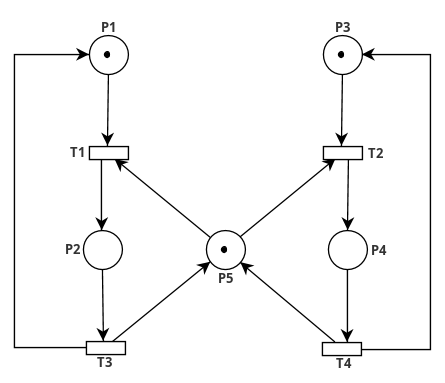
\includegraphics[width=0.7\linewidth]{images/rdp_p_invariantes.png}
    \caption{P-invariantes de la red de Petri}
    \label{fig:rdp_p_invariantes}
\end{figure}

\noindent Tras el análisis de la red , se obtienen las siguientes invariantes de plazas:
 
\begin{equation}
   \begin{array}{cc}
       m(P_1) + m(P_2) = 1  \\
       m(P_3) + m(P_4) = 1   \\
       m(P_2) + m(P_4) + m(P_5) = 1 
   \end{array}
\end{equation}

El primer ítem expresa que la sumatoria de tokens en las plazas $P_1$ y $P_2$ siempre será igual a uno, afirmación completamente observable al mirar la red de la figura \ref{fig:rdp_p_invariantes}. Estas declaraciones implican la siguiente consecuencia:

\begin{equation}
   I . x = 0
\end{equation}

\noindent donde $I$ es la matriz de incidencia y $x$ es un vector característico de un subconjunto $Q$ de las plazas que forman parte de la invariante (un uno en una posición indica que esa plaza es parte de la invariante y un cero indica lo contrario). A partir de esto surge la siguiente fórmula:

\begin{equation}
    \sum_{P \in \bullet t \cap Q} W(p,t) = \sum_{P \in t \bullet \cap Q} W(t,p)
\end{equation}

\noindent la cual puede ser expresada en función de un vector t de la siguiente manera:

\begin{equation}
    \sum_{P \in \bullet t \cap Q} t(p) = \sum_{P \in t \bullet \cap Q} t(p)
\end{equation}

\noindent Esto quiere decir que:

\begin{equation}
    \sum_{P \in (t \bullet \cup \bullet t) \cap Q} t(p) = 0 \ \ y \  \sum_{P \in Q} t(p) = 0
\end{equation}

Si reemplazamos $Q$ por los vectores característicos $I_q$ , estas dos igualdades pueden escribirse como:

\begin{equation}
    \sum_{P \in Q} t(p) I_q(p) = 0 \ \ y \  \sum_{p \in P} t(p)I(p) = 0
\end{equation}

\noindent Lo cual es simplemente la definición del producto escalar entre dos vectores:

\begin{equation}
    t.I_q = 0
\end{equation}

\noindent Como los disparos son arbitrarios, podemos establecer la siguiente relación:
\begin{equation}
    t_j I_q; \forall \ t_j \ \in \ T \Longleftrightarrow \ I^T I_q = 0
\end{equation}

\noindent donde $I^T$ es la matriz de incidencia transpuesta.

\subsubsection{T-invariantes}
Un \textbf{invariante de transición} ó \textbf{T-invariante} es el conjunto de transiciones que deben dispararse para que la red de Petri retorne a su estado inicial.

Como se mencionó en el apartado anterior, para el cálculo de las P-invariantes se hace uso de la ecuación $I . x = 0$, siendo $I$ la matriz de incidencia y $x$ un vector característico constituido por las plazas que forman parte de la invariante. En este caso, para el cálculo de los vectores que constituyen las T-invariantes, la ecuación asociada será similar a las P-invariantes, a diferencia que se hace uso de  $I^T$ en vez de $I$:

\begin{equation}
    I^T . x = 0
\end{equation}

Aquí, a diferencia de las P-invariantes, el vector x está constituido por el conjunto de transiciones que deben dispararse para que la red retorne al estado inicial. Un "1" en una posición indica que esa transición es parte de la invariante y un "0" indica lo contrario.

Tomando la figura \ref{fig:rdp_p_invariantes} como ejemplo y se obtienen las siguientes invariantes de transiciones:

\begin{equation}
    T-invariantes = 
    \begin{pmatrix}
         T0 & T1 & T2 & T3  \\
         0 & 1 & 0 & 1  \\
         1 & 0 & 1 & 0  
    \end{pmatrix}
\end{equation}

Ambos vectores cumplen la condición planteada ($I^T .\ x = 0$) y si se observa la imagen en cuestión, se puede apreciar que la red retorna a su estado inicial si las transiciones especificadas en los vectores se disparan.

\section{Concurrencia y sincronización}
En los sistemas de computación actuales conviven múltiples procesos que cooperan para lograr determinados objetivos y compiten por recursos del sistema, entre ellos el procesador, la memoria RAM, los puertos de entrada/salida, etc.\\
Dado que generalmente el numero de procesos de un sistema supera ampliamente el numero de recursos, se deben establecer formas de comunicación y sincronización entre ellos que hagan que el sistema funcione correctamente. 

\par En ésta sección se definirá cuando dos programa son concurrentes y/o paralelos y las condiciones que deben cumplirse para que dos secciones de código fuente puedan ser ejecutadas de manera concurrente. Luego, se verá que la ejecución concurrente de procesos trae aparejados ciertos problemas como el interbloqueo y la inanición.\\
Por esta razón deben ejecutarse ciertos mecanismos de control para garantizar la correcta ejecución de los programas, entre ellos, los semáforos y monitores.\\
El objetivo de esta sección es que el lector adquiera una idea general sobre la programación concurrente y sobre los problemas inherentes a la misma.

\subsection{Concurrencia y paralelismo}
Dos procesos serán concurrentes cuando la primera instrucción de uno de ellos se ejecuta después de la primera instrucción de otro proceso y antes de la última.
No es necesario que estos se ejecuten al mismo tiempo, basta con el hecho de que se intercalen sus instrucciones. En caso de ejecutarse al mismo tiempo se dice que hay programación paralela.
La programación concurrente es un paralelismo potencial, dependiente del hardware que lo soporte  \cite{mendez}.

\subsubsection{Problemas inherentes a la programación concurrente}
La intercalación de instrucciones de diferentes procesos, debe ser bien manejada y controlada dado que puede producir mal funcionamiento del sistema. Los problemas inherentes a la concurrencia son:
\begin{itemize}
    \item \textbf{Exclusión mutua}: Se debe garantizar que si un proceso adquiere el recurso los demás deberán esperar hasta que sea liberado.

    \item \textbf{Condición de sincronización}: Hay situaciones en las que un proceso debe esperar que ocurra algún determinado evento para poder continuar. Por ello se debe garantizar que si el evento \textbf{no} ocurrió, el proceso \textbf{no} continúe. 
    
    \item \textbf{Interbloqueo}: Esta situación se produce cuando todos los procesos están esperando un evento que nunca ocurrirá. Se debe garantizar que estas situaciones no ocurran.
    
    \item \textbf{Inanición}: En este caso, el sistema en su conjunto hace progresos, pero existe un grupo de procesos que nunca progresaran pues no se les otorga tiempo de procesador para hacerlo.
\end{itemize}

\subsubsection{Exclusión mutua}
La exclusión mutua implica que dos o más procesos intentan acceder a un único recurso compartido entre ellos pero solo uno puede acceder a cada instante.
Cuando se da un caso de estas características, se desea que todo lo que necesite hacer unos de los procesos sobre el recurso se realice de manera indivisible y luego lo deje disponible para que otro proceso ejecute sus instrucciones sobre el recurso.
\par A la porción de código que se desea que se ejecute de manera indivisible o atómica se le llama \textbf{sección crítica}. Se debe lograr que todas las instrucciones dentro de la sección crítica se ejecuten en exclusión mutua lo que implica que el hecho de que cuando uno de los procesos este ejecutando esa porción de código el resto no podrá hacerlo. \\
\\
\textbf{Solo uno de los procesos podrá estar en la sección crítica en un instante dado.}

\begin{figure}[H]
    \centering
    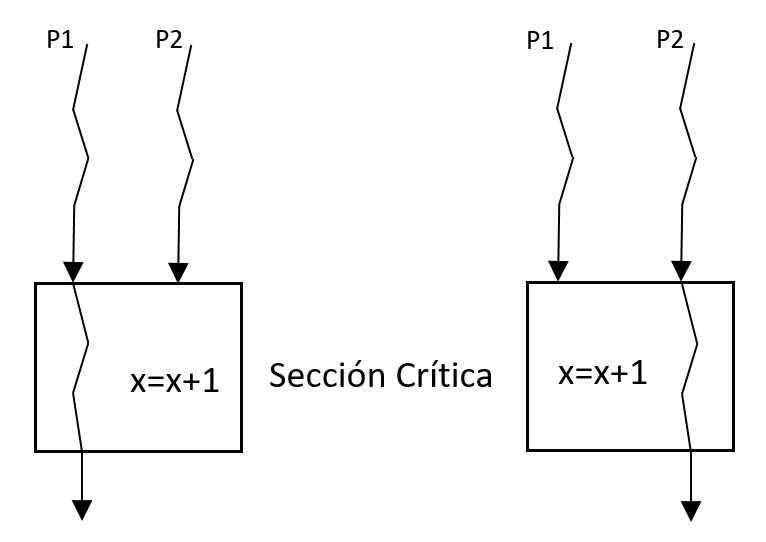
\includegraphics[scale=0.4]{images/seccion_critica.jpg}
    \caption{Sección crítica}
    \label{fig:seccion_critica}
\end{figure}

En la figura \ref{fig:seccion_critica} se observa como dos procesos $P1$ y $P2$ intentan ejecutar una porción de código de una sección crítica. La imagen de la izquierda (a) muestra que el proceso $P1$ consigue ingresar a ejecutar la sección crítica. La imagen de la derecha (b) muestra que el proceso $P2$ puede ingresar solo cuando el proceso $P1$ ya no esta en la misma.

\noindent La exclusión mutua se puede representar de la siguiente manera.
\begin{figure}[H]
    \centering
    \includegraphics[scale=0.7]{images/rdp_seccion_crítica.png}
    \caption{Sección crítica}
    \label{fig:rdp_seccion_crítica}
  \end{figure}

En la figura \ref{fig:rdp_seccion_crítica} la plaza \textit{MUTEX} esta limitada a un único token y el análisis de invariantes de plazas demuestra formalmente la propiedad de exclusión mutua entre los procesos $P1$ y $P2$. 

\begin{equation}
    m(EjecutandoSCP1) + m(MUTEX) + m(EjecutandoSCP2) = 1
\end{equation}

\subsection{Interbloqueo}
En un sistema donde los procesos compiten por limitados recursos, pueden producirse demandas contradictorias de los mismos. Por ejemplo, si existen dos procesos, \textit{A} y \textit{B}, y dos recursos \textit{R1} y \textit{R2}, y ambos procesos necesitan los dos recursos para proseguir, si el proceso \textit{A} toma el recurso \textit{R1} y el \textit{B} el recurso \textit{R2}, ambos procesos se bloquearan a la espera del otro recurso, pero ninguno liberará el recurso que posee hasta no conseguir los dos. A esta situación se la conoce como interbloqueo. 

\subsubsection{Condiciones para producir interbloqueo: }
\noindent Deben presentarse tres condiciones de gestión para que sea posible un interbloqueo:
\begin{enumerate}
    \item \textit{Exclusión mutua}: sólo un proceso puede utilizar un recurso en cada momento. Ningún proceso puede acceder a un recurso que se ha asignado a otro proceso.
    
    \item \textit{Retención y espera}: un proceso puede mantener los recursos asignados mientras espera la asignación de otros recursos.
    
    \item \textit{No apropiación}: ningún proceso podrá ser forzado a abandonar un recurso que retiene.
    
    \item \textit{Espera circular}: existe una cadena cerrada de procesos donde cada proceso retiene un recurso que necesita un proceso que le sigue en la cadena.
\end{enumerate}

Las tres primeras condiciones son necesarias pero no suficientes para que exista interbloqueo.
La cuarta es una consecuencia potencial de las tres primeras y, en caso de darse, generará una \textbf{espera circular irresoluble}. Esta es de hecho la definición de interbloqueo.

\subsection{Sincronización}
Para solucionar los problemas inherentes a la programación concurrente, se utiliza lo que se llama \textit{sincronización entre los procesos} . \\
Se habla de sincronización , en general, cuando determinados fenómenos ocurren o deben ocurrir en un determinado orden o a la vez.
\par Para la computación, la sincronización es representada por las señales que se envían los procesos para colaborar entre ellos o para indicar el estado de recursos compartidos, para indicar que un evento o acción ocurrió o no y determinar la continuidad o no de un proceso, etcétera.
\par La condición de sincronización puede definirse como la propiedad requerida para que un proceso no realice ninguna acción o evento hasta que otro proceso realice una determinada acción o evento.

\subsubsection{Semáforos}
Los semáforos son un sistema de señales simples utilizadas por los procesos para comunicarse entre ellos y lograr la sincronización requerida.
Estos tienen una variable de sincronización, del tipo entero no negativo, que indica la cantidad de recursos disponibles. Sobre esta se realizan dos tipos de operaciones:

\begin{itemize}
    \item \textit{wait}: decrementa el valor del semáforo solo si este es mayor que cero. Este proceso indica que se utiliza uno de los recursos que controla el semáforo. Si el valor del semáforo al momento de ejecutar la operación \textit{wait} es cero, indica que no hay recursos disponibles y el proceso deben bloquearse hasta que se libere alguno.
    \item \textit{signal}: es la acción de liberar un recurso que estaba siendo utilizado. En caso de haber algún proceso bloqueado en el semáforo se lo despierta para que utilice el recurso. De no existir algún proceso, se incrementa el valor del semáforo.
\end{itemize}

Los semáforos son primitivas con las cuales es difícil expresar una solución a grandes problemas de concurrencia, ya que tienen algunas debilidades:
\begin{itemize}
    \item La omisión de una de las primitivas puede corromper el funcionamiento de un sistema concurrente.
    \item El control de concurrencia es responsabilidad del programador.
    \item Las primitivas de control se encuentran esparcidas por todo el código, lo que hace muy difícil la corrección de errores y el mantenimiento del mismo.
\end{itemize}

Debido a estas razones existe otro mecanismo de software para el control de concurrencia denominado \textbf{monitor}.

\subsubsection{Monitores}
Como se dijo, los semáforos, generalmente se encuentran dispersos en el código, lo que lo hace más confuso y muchas veces es difícil notar cual es el recurso compartido y determinar si está correctamente sincronizado. Por ello, se necesita un sistema que sea igual de versátil que los semáforos pero que permita efectuar un control más estructurado de la exclusión mutua. Una herramienta con estas características fue propuesta por \textit{C.A.R Hoare} en 1975 y es conocida como \textbf{\textit{monitor}}.\\
Un \textbf{monitor} es un mecanismo de abstracción de datos, lo que permite representar de forma abstracta un recurso compartido mediante variables que indican su estado. El acceso a esas variables solo es posible a través de un conjunto de funciones/métodos que el monitor exporta al exterior.\\

Un monitor se compone de los siguientes elementos:
\begin{itemize}
    \item Un \textit{conjunto de variables} locales que pueden denominarse permanentes. Se utilizan para almacenar el estado interno del recurso que representa el monitor. Se denominan permanentes ya que permanecen sin modificarse entre dos llamadas consecutivas al monitor y solo pueden ser accedidas dentro del mismo.
    
    \item Un \textit{código de inicialización} que se ejecuta antes que la primera instrucción ejecutable del programa y su fin es inicializar las variables permanentes. 

    \item Un \textit{conjunto de procedimientos internos} que manipulan las variables permanentes.
    
    \item Una \textit{declaración de los procedimientos} que son \textit{exportados} y pueden ser accedidos por los procesos activos externos.
\end{itemize}

\paragraph{Exclusión mutua en monitores}
\hfill
\par El control de la exclusión mutua en un monitor se basa en la existencia de una cola asociada al mismo que se denominara \textit{cola del monitor}. La gestión de esta cola se realiza de la siguiente manera:

\begin{enumerate}
    \item Cuando un proceso activo está dentro del monitor (ejecutando alguno de los procedimientos del mismo) y aparece otro proceso activo que intenta ejecutar otro (o el mismo) procedimiento, el código de acceso al monitor bloquea el proceso que realiza la llamada y lo inserta en la cola del monitor (con política FIFO). Así, se impide que dos procesos estén al mismo tiempo dentro del monitor.

    \item Cuando un proceso activo abandona el monitor, este ultimo selecciona el proceso que esta al frente de la cola del monitor y lo desbloquea para que comience a ejecutar las operaciones que le solicitó al monitor. Si la cola estaba vacía, el monitor queda libre y cualquier proceso activo que llame alguno de sus procedimientos entrará al monitor.
\end{enumerate}

Esto asegura que las variables compartidas nunca son accedidas concurrentemente. Una cuestión importante es que la responsabilidad de bloquear un proceso es del monitor y no del proceso.
Al comparar este sistema con un semáforo se ve que en el caso de los semáforos son los propios procesos activos los que manejan las políticas de acceso a variables compartidas.

\paragraph{Condición de sincronización en monitores}
\hfill
\par El procedimiento anterior sólo controla la exclusión mutua, es decir, pueden haber casos donde un proceso activo tenga acceso al monitor (ha obtenido la exclusión mutua al mismo) pero no puede seguir su ejecución debido a alguna razón, tal como un \textit{buffer} lleno que no puede ser escrito. En estos casos, es necesario bloquear ese proceso y permitir que otro ingrese al monitor. Para realizar esto surgen nuevos componentes que deben formar parte del monitor:

\begin{itemize}
    \item Variables de condición
    \begin{itemize}
        \item Las mismas son declaradas en el monitor. 
        \item Deben ser privadas. 
        \item Tienen una cola \textit{FIFO} asociada.
    \end{itemize}
    \item Operaciones sobre las variables de condición
    \begin{itemize}
        \item \textit{Delay}
        \item \textit{Resume}
        \item \textit{Empty}
    \end{itemize}
\end{itemize}

La operación delay se realiza sobre una variable de condición. Si se supone la existencia de una variable C, al realizar \textit{delay(C)}, el proceso que la ejecutó libera el mutex del monitor, se bloquea y se envía al final de la cola asociada a la condición C. A diferencia de la operación wait que se utiliza en los semáforos, delay bloquea al proceso incondicionalmente.\\

\par La operación resume, cuando se realiza sobre una variable C, libera al primer proceso que ejecutó \textit{delay(C)}. Si la cola está vacía, resume es una operación nula. Por otra parte, la función empty simplemente devuelve un valor boolean true si una cola se encuentra vacía o false en caso contrario.\\

Con lo dicho hasta este punto, se podría decir que si un proceso que se está ejecutando dentro del monitor ejecuta una operación \textit{resume(C)}, se desbloqueará un proceso de esa cola que continuará con su ejecución dentro del monitor también. Esto lleva a una situación con dos procesos dentro del monitor, lo que violaría la exclusión mutua. Para evitar esto, el proceso que ejecuta el \textit{resume} cederá la exclusión mutua al recien desbloqueado. Y espera en una cola diferente llamada \textbf{cola de cortesía} hasta que el proceso recién desbloqueado por el \textit{resume(C)} termine su ejecución teniendo preferencia por sobre los procesos esperando en otras colas.

\begin{figure}[H]
    \centering
    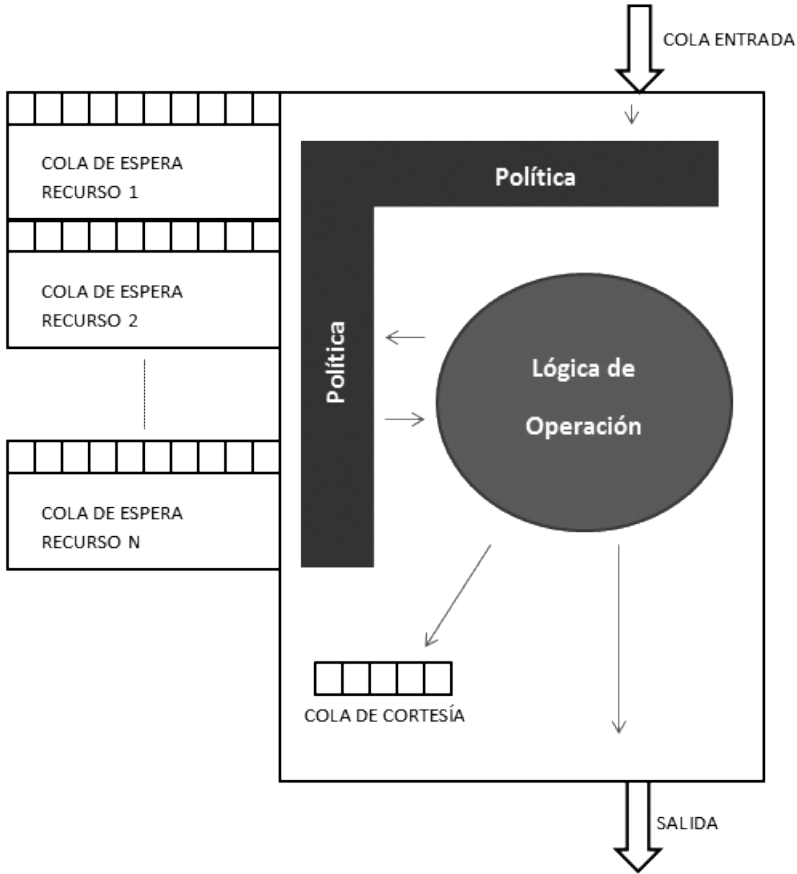
\includegraphics[scale=0.5]{images/monitor_mico.png}
    \caption[Monitor.]{Figura adaptada del Proyecto Integrador \textit{Desarrollo de IP cores con procesamiento de Redes de Petri Temporales para sistemas multicore en FPGA}}
    \label{fig:monitormico}
\end{figure}

\subsubsection{Implementación de monitores con redes de Petri}
Es posible ver a un monitor formado por dos secciones: primero, la referida a la política de colas que se debe ejecutar para lograr que sólo un proceso esté en el monitor, que se bloqueen los procesos que no tienen los recursos y que se desbloqueen los que obtuvieron los recursos, y segundo, la lógica con que se administran los recursos.\\
En la figura \ref{fig:monitormico} se puede observar que existe una cola de entrada, para los procesos que aún no ingresaron al monitor y desean hacerlo, una serie de colas, una por cada recurso (cada condición de sincronización) y una cola de cortesía para que  proceso dentro del monitor pueda, de manera segura, ceder la exclusión mutua al cambiar el estado de un recurso.\\

\par \textbf{\textit{Una red de Petri puede realizar el trabajo de la lógica del monitor}}, es decir, la administración y sincronización de recursos disponibles; esto es cuando el vector de estado que resultó del disparo no tiene componentes negativas es porque los recursos están disponibles, el disparo de la transición solicitada conduce a un nuevo estado valido. De no ser así, en caso de existir algún valor negativo en el nuevo vector de estado, se llegó a un estado no válido que indica que el recurso no está disponible. Además el vector de estado indica si el disparo ha devuelto o tomado recursos. Si la cantidad de tokens para un recurso dado disminuye, significa que se han tomado recursos, en caso contrario, que se han devuelto recursos.

\begin{figure}[H]
    \centering
    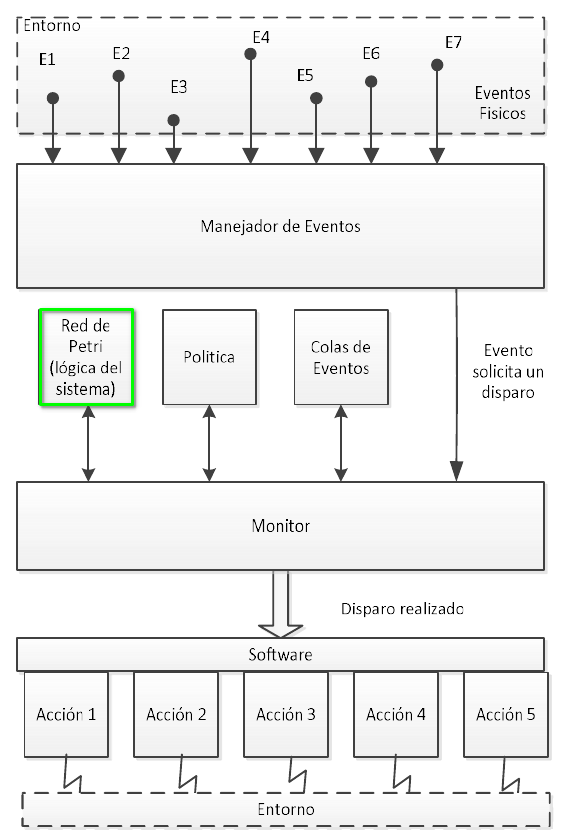
\includegraphics[scale=0.5]{images/monitor_mico_1.png}
    \caption[Monitor.]{Monitor figura adaptada del paper publicado por \textit{Micolini, Orlando \& Ventre, Luis \& Cebollada, Marcelo \& Eschoyez, Maximiliano}}
    \label{fig:monitormico1}
\end{figure}

Por lo tanto, el monitor integra la red de Petri (lógica), la política y las acciones, conformando un sistema heterogéneo. La importancia de la metodología aquí planteada radica en desacoplar la lógica de la política y las acciones, con el fin de obtener un sistema resultante modular, simple, mantenible y verificable. 

En la figura \ref{fig:monitormico1} se expone la arquitectura modular de un sistema reactivo y guiado por eventos.

\newpage
\chapter{Desarrollo}

Este proyecto ilustra la concepción y construcción de un robot móvil pequeño. Se detallaran todas las etapas de desarrollo del mismo, partiendo de los componentes básicos hasta el producto terminado. Para el desarrollo de este proyecto, se realizarán iteraciones donde en cada una se sigue un ciclo que incluye los requerimientos que se aborda, el desarrollo, las pruebas y los resultados obtenidos. A continuación, se detalla cada una de las etapas de una iteración típica. Un enfoque iterativo permite ajustar y mejorar continuamente el proyecto, asegurando que se cumplan todos los requerimientos y objetivos.

En primera instancia se identifican los requerimientos que se abordan en la iteración. Estos requerimientos pueden repetirse en iteraciones sucesivas en caso de necesitar un ajuste o replanteo. Con los requerimientos en mente, se procede a elaborar una solución detallada y se planifica su implementación.

Para verificar y validar el diseño durante el proceso de desarrollo, se llevan a cabo las pruebas del componente o funcionalidad desarrollada y se documentan, garantizando que funcione correctamente y cumpla con las expectativas. Los resultados obtenidos se analizan para determinar si se ha alcanzado el objetivo de la iteración.

Finalmente, se elabora una conclusión de la iteración, en la que se resumen los resultados obtenidos y las lecciones aprendidas. Esta conclusión ayuda a identificar cualquier mejora necesaria o puntos que requieran revisión en futuras iteraciones.

\newpage
\section{Iteración 0: Decisiones preliminares}
\subsection{Introducción}
En esta iteración vamos plantear la elección que realizamos para todos los componentes que componen el robot, los opciones que contemplamos para la implementación y el motivo de las elecciones.

\subsection{Requerimientos}

En esta iteración abordaremos los siguientes requerimientos funcionales:

\begin{center}
    \begin{tabular} {
        | >{\centering\arraybackslash}m{1cm}
        | >{\centering\arraybackslash}m{13cm} |}
        \hline \rowcolor{test_header_color}
            ID & Descripción \\
        \hline
            RF4 & El robot debe poder realizar trayectorias en línea recta y curvas. \\
        \hline
            RF6 & El robot debe recibir y enviar información mediante comunicaciones inalámbricas. \\
        \hline
            RF8 & Debe poder ubicarse al robot en el plano de forma precisa. \\
        \hline
    \end{tabular}
\end{center}

   Por otra parte, el requerimiento no funcional que abordaremos es:

\begin{center}
    \begin{tabular} {
        | >{\centering\arraybackslash}m{1cm}
        | >{\centering\arraybackslash}m{13cm} |}
        \hline \rowcolor{test_header_color}
            ID & Descripción \\
        \hline
            RNF1 & Debería tener tiempos de respuesta aceptables para el buen funcionamiento del sistema de control. \\
        \hline
    \end{tabular}
\end{center}

\subsection{Desarrollo}

\subsection{Relevamiento del Proyecto Integrador Hermes III}

El robot Hermes III es la última versión de la familia de robots desarrollada dentro del laboratorio de arquitectura de computadoras. Este también incorpora sistemas del modelo anterior y plantea una mejora sobre ellos, en este caso sobre el sistema de control que comanda el robot móvil y la implementación de un sistema operativo robótico (ROS) el cual es un framework para Linux que está diseñado exclusivamente para el desarrollo de robots. \cite{micolini2022hermes}

El uso del sistema operativo ROS abre la posibilidad de usar software dedicado al desarrollo de robots móviles y también a la incorporación de componentes como ser el módulo de cámara Kinect desarrollado por Microsoft para la consola Xbox.

El conjunto ya mencionado da paso a la implementación e innovación más importante del proyecto, la localización y mapeo en simultáneo (SLAM), brindándole al robot la posibilidad de moverse sobre un superficie y crear un mapa de su entorno, provocando que en cada nueva iteración pueda mejorar su desplazamiento y localización en la superficie de movimiento.

El software se ejecuta sobre una placa NVIDIA Jetson TK1, la cual ofrece un gran poder de cómputo que es necesario para sostener y correr de forma efectiva tanto el sistema operativo como el algoritmo de SLAM. La desventaja es su alto precio, lo que aumenta el costo de construcción del robot y por lo tanto disminuye la posibilidad de pensar en un flota de estos equipos.

\subsubsection{Elección de microcontrolador}

Dentro de las características del modelo anterior de la familia Hermes, se destacaba la gran cantidad hardware por el cual estaba compuesto, y por ende, el gran costo para su replicación e implementación.

Para esta nueva edición se decidió reducir la cantidad de componentes que lo integran, en cuanto al procesamiento se refiere, y llevarlo a un modelo que se acerque mas a la Industria 4.0 donde los dispositivos se conectan a Internet y es allí donde mandan reportes y reciben instrucciones. Es por eso que se optó por la utilización del microcontrolador ESP-32 el cual proporciona un API bastante completa y por en ende un gran abanico para que el desarrollador despliegue todo su potencial. \cite{kolban2017kolban}

\begin{figure}[H]
   \centering
   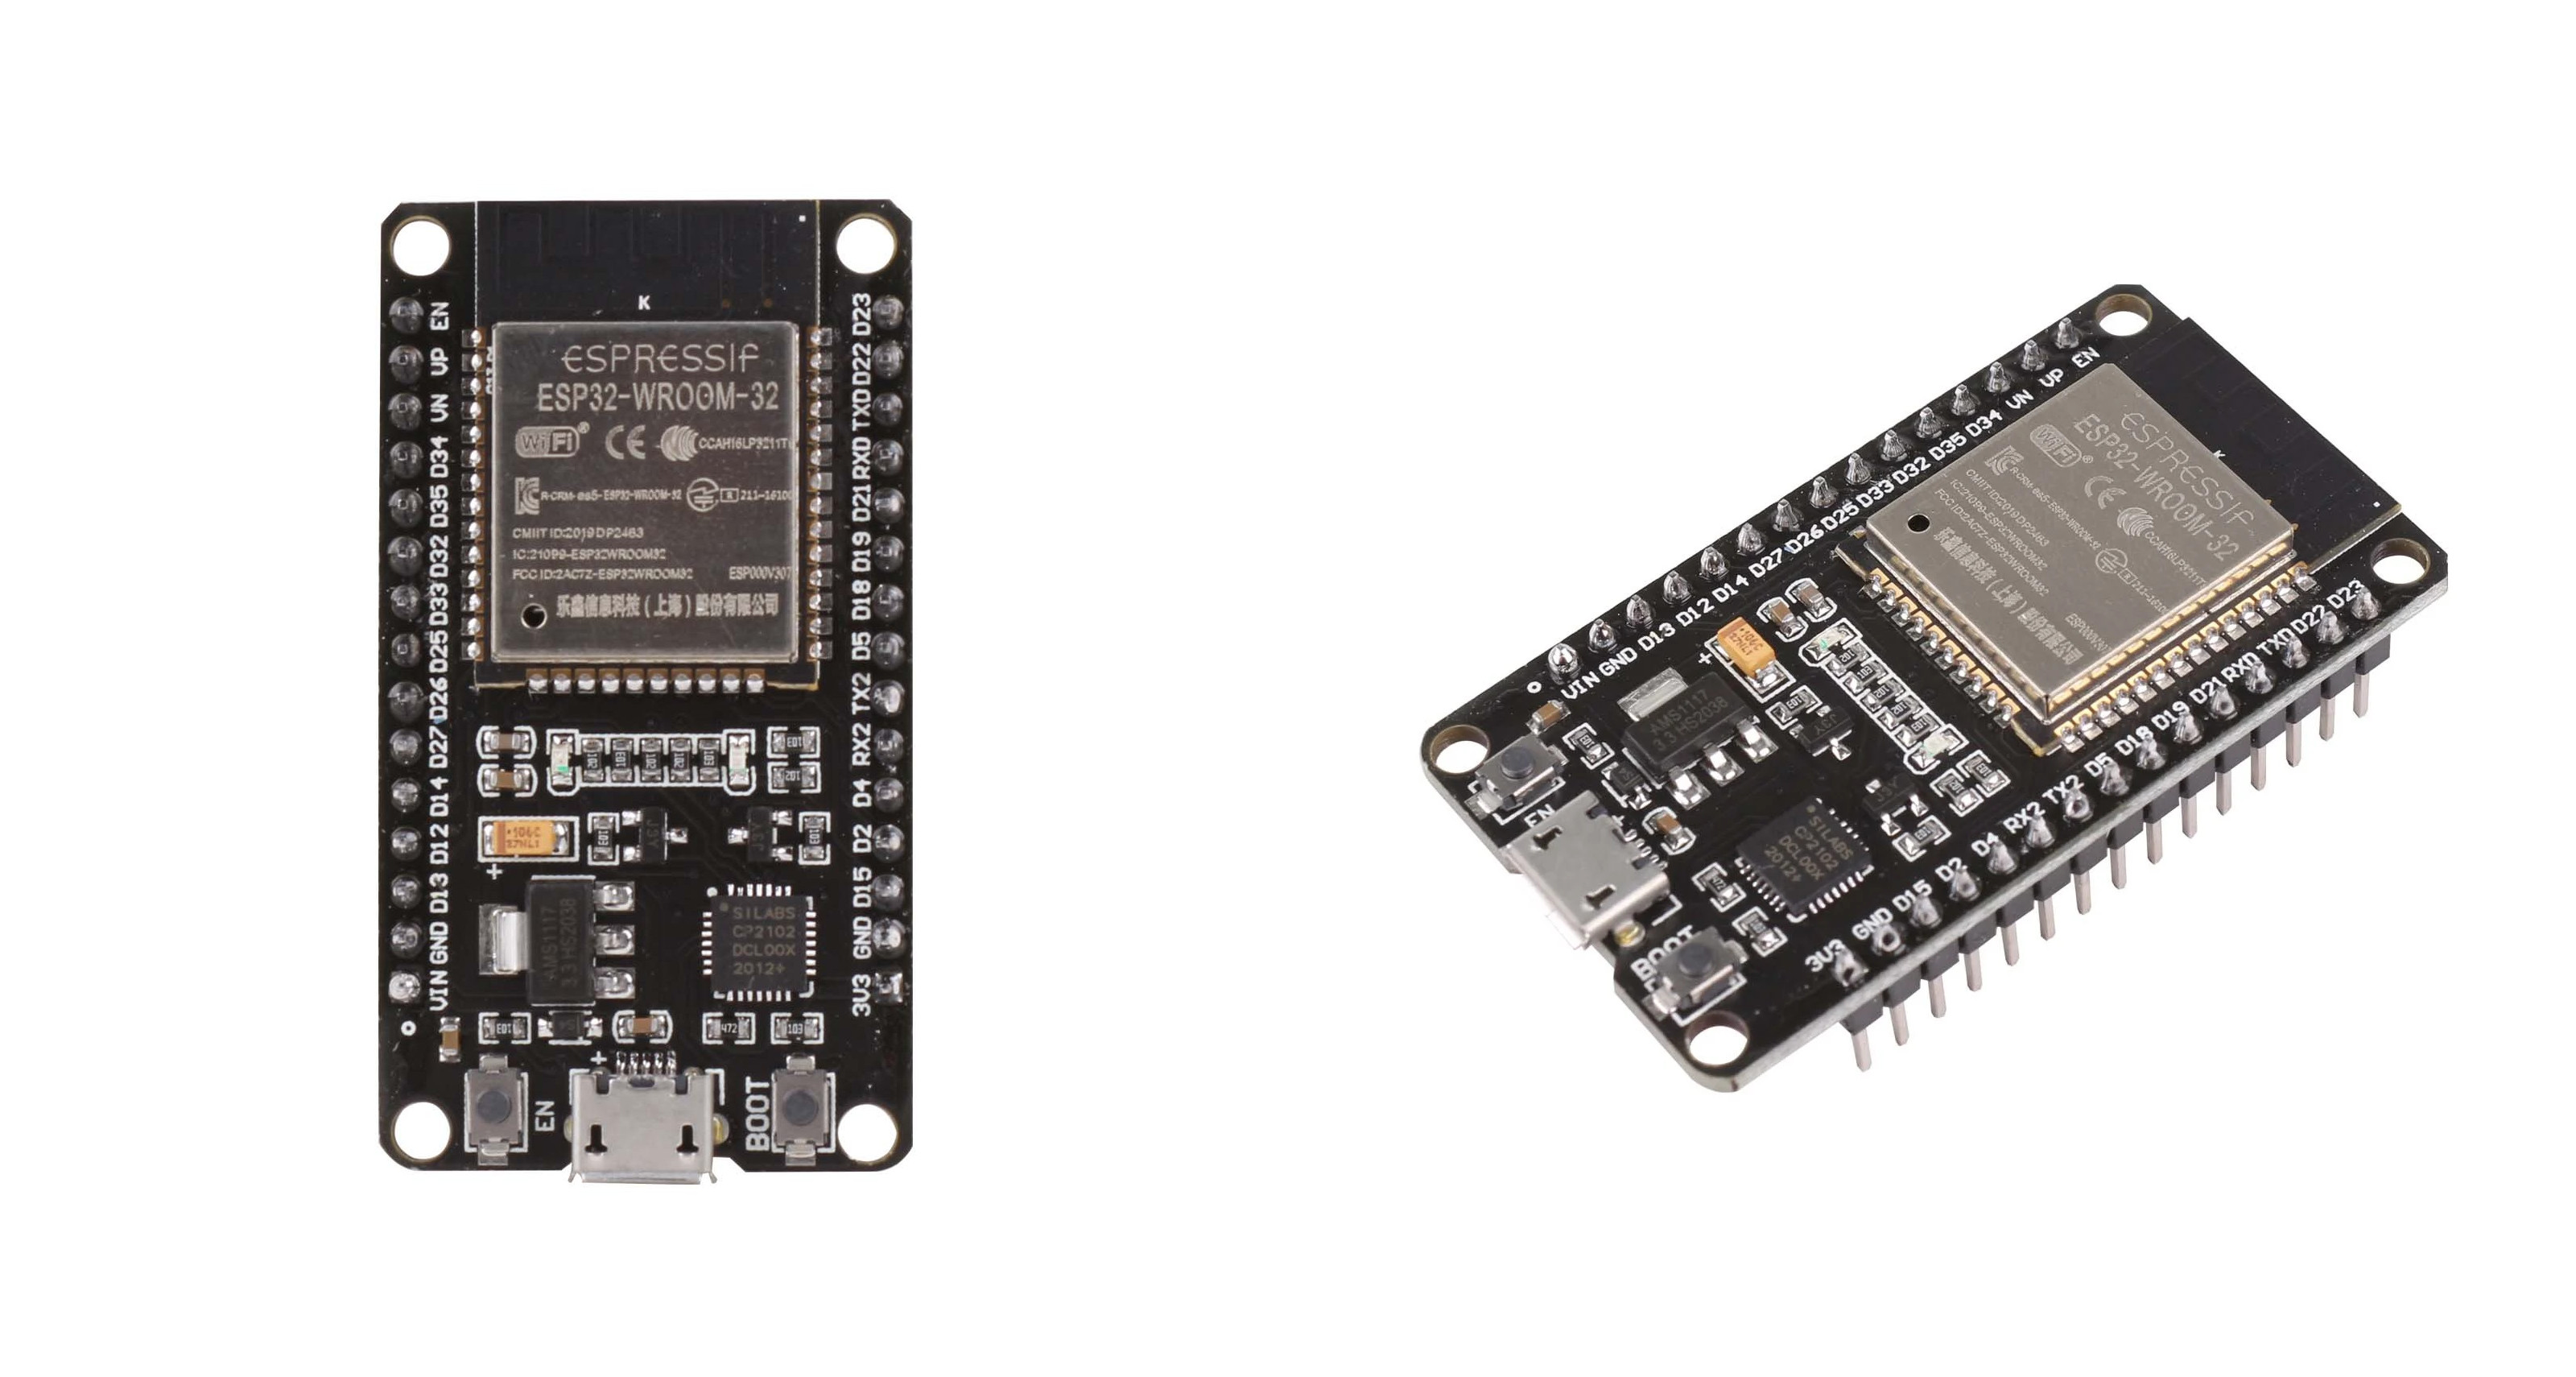
\includegraphics[width=0.7\linewidth]{images/esp32-micro.jpg}
   \caption{Microcontrolador ESP32}
   \label{fig:microcontrolador}
\end{figure}

\subsubsection{Sistema Operativo}

La decisión de utilizar FreeRTOS como sistema operativo para el desarrollo de este proyecto se fundamenta en varias consideraciones claves. Primero, FreeRTOS está integrado de manera nativa en el framework ESP-IDF de Espressif, lo que facilita enormemente el desarrollo y la integración de funcionalidades en tiempo real. Al utilizar la API de Espressif, se aprovechan componentes y servicios que ya están optimizados para trabajar con FreeRTOS, lo que se traduce en una mayor estabilidad y rendimiento en aplicaciones críticas.

FreeRTOS permite una gestión eficiente de tareas, permitiendo la concurrencia y la sincronización de procesos de manera robusta y controlada. Esto es esencial para aplicaciones que requieren una respuesta rápida a eventos externos, como la gestión de sensores, la comunicación inalámbrica y la realización de múltiples operaciones simultáneamente. La modularidad y escalabilidad que ofrece FreeRTOS permite desarrollar soluciones complejas sin incurrir en sobre costos de recursos, lo que es especialmente valioso en sistemas embebidas con limitaciones de hardware. \cite{barry2016mastering}

El uso de FreeRTOS está respaldado por un amplio ecosistema de documentación y soporte, facilitando el desarrollo, la depuración y el mantenimiento de aplicaciones en el microcontrolador ESP32. Esta sinergia entre el hardware y el sistema operativo garantiza una integración fluida y optimizada para las exigencias de aplicaciones modernas en sistemas embebidos y soluciones IoT, lo que se ajusta perfectamente al desarrollo de este proyecto.

\begin{figure}[H]
  \centering
  
\includegraphics[width=0.4\linewidth]{images/freertos.jpg}
  \caption{Sistema operativo usado por los microcontroladores}
  \label{fig:sistema_operativo}
\end{figure}

\subsubsection{Elección de motores}

El sistema de locomoción es el responsable de la traslación del robot. Las configuraciones más comunes son las siguientes: diferencial, sincrónico, triciclo, ackerman y omnidireccional.

Como nosotros tomamos como base la estructura ya definida para el robot Hermes III, adoptamos el sistema mecánico de locomoción omnidireccional, el cual permite mayor libertad de movimiento que los sistemas de ruedas clásicos, Los robots que implementan este sistema pueden moverse en cualquier dirección sobre el plano y en cualquier momento sin la necesidad de hacer movimientos previos para modificar su trayectoria. Requiere ruedas que permitan movimientos en más de una dirección. Este sistema puede ser implementado con tres o cuatro ruedas.

Las ruedas omnidireccionales ruedan en el sentido de avance, pero, también se pueden desplazar lateralmente con gran facilidad como se observa en la siguiente figura:

\begin{figure}[H]
    \centering
    \includegraphics[width=0.25\linewidth]{images/omni-wheel-wikipedia.png}
    \caption{Rueda omnidireccional}
    \label{fig:rueda_omnidireccional}
\end{figure}

Los actuadores tienen por misión generar el movimiento de los elementos del robot según las órdenes dadas por la unidad de control. De manera general, los actuadores utilizados en robótica pueden emplear energía neumática, hidráulica o eléctrica. Las características de control, sencillez y precisión de los accionamientos han hecho que los actuadores eléctricos sean los más usados. Dentro de los actuadores eléctricos pueden distinguirse tres tipos diferentes: \\

\textbf{Motores de corriente continua (DC):}
\begin{itemize}
   \item Controlados por inducción
   \item Controlados por excitación
\end{itemize}

\textbf{Motores de corriente alterna (AC):}
\begin{itemize}
   \item Síncronos
   \item Asíncronos
\end{itemize}

Se opta por motores de corriente continua, como el que se muestra en la figura siguiente, pues el torque generado es proporcional a la diferencia de potencial aplicado a los terminales de alimentación y el sentido de giro depende de la polaridad, facilitando de este manera el control. El modelo de motor elegido se muestra en la imagen debajo, es un motorreductor de $12V\ @\ 100\ RPM$.

\begin{figure}[H]
    \centering
    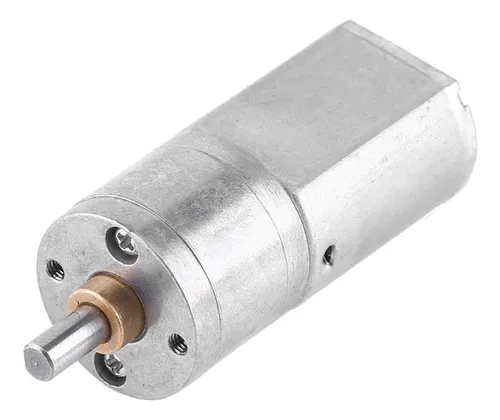
\includegraphics[width=0.35\linewidth]{images/motorreductor.png}
    \caption{Motorreductor}
\end{figure}


Este tipo de motores pequeños y de bajo costo generalmente presentan como inconveniente que no publican sus curvas. Para resolver este inconveniente se realizaron distintos experimentos. Esencialmente se construyó un montaje que consta de una polea con un peso conocido, que no es más que un recipiente con agua como muestra la siguiente figura, la polea se fija al eje del motor para realizar los experimentos.

Se realizaron distintas corridas variando la tensión y corriente, se tomaron mediciones de velocidad y torque. Con estos datos se construyeron las curvas de rpm-torque y corriente-torque, como se muestra la siguiente tabla:

\begin{center} \begin{tabular}{|c|c|c|}
   \hline \rowcolor{test_header_color}
       Tensión & Velocidad & Torque \\
   \hline
       3V & 25 RPM & 0,3 Kg*cm\\
   \hline
       6V & 67 RPM & 1 Kg*cm\\
   \hline
       12V & 96 RPM & 2 Kg*cm\\
   \hline
\end{tabular} \end{center}

Con estos experimentos, también, se midió la respuesta del sistema a un escalón, detallado en la siguiente iteración.

\begin{figure}[H]
    \centering
    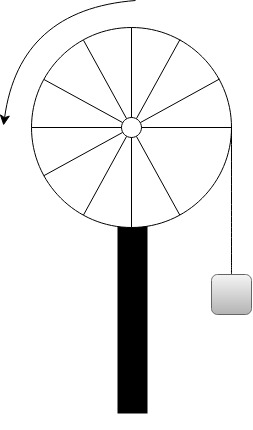
\includegraphics[width=0.25\linewidth]{images/medicion_rpm.jpg}
    \caption{Montaje para medir el torque}
    \label{fig:medicion_torque}
\end{figure}

Para la alimentación de los motores es necesario un circuito integrado especial que permite manipular de manera segura la corriente eléctrica de los motores y a su vez brinde la posibilidad de controlar la polaridad de los bornes donde se conectan los mismos para cambiar su sentido de giro.

Esta solución se ofrece en el mercado en el integrado comúnmente denominado "Driver Dual para Motores L298N", también conocido como "puente H", el cual posee a su vez un regulador de voltaje LM7805 para alimentar la parte lógica del integrado L298N.

El sentido de giro de un motor estará definido por dos pines cuyos valores establecerán la polaridad de los terminales de alimentación del motor respectivamente. Existen dos pares de pines por cada motor.

Para el control de estos integrados vamos a usar cuatro canales PWM del microcontrolador ESP-32, los cuales van a establecer el sentido de giro y fuerza del motor.

\subsubsection{Sensores rotativos} \mbox{} \vspace{10pt} \\
Un sensor es un dispositivo eléctrico y/o mecánico capaz de convertir magnitudes físicas, como la luz, velocidad, aceleración, presión, temperatura, etc. En otra magnitud, normalmente eléctrica, que sea posible manipular y cuantificar.

Para nuestro caso en particular, usamos los sensores para medir la velocidad de los motores. Como el objetivo es construir un sistema de lazo cerrado que controle la velocidad de los motores con el fin de aproximar la trayectoria calculada.

Para medir la velocidad en revoluciones por minuto (RPM), se colocó, en el eje del motor, una rueda con patrón impreso el cual es detectado por un sensor infrarrojo (opto acoplador de ranura). El patrón impreso consta de líneas perforadas, ranuras, en la rueda con el fin de generar interrupciones. Se realizaron 24 ranuras en cada rueda para poder realizar el cálculo de la distancia recorrida.

Para realizar la medición de RPM se experimentó tres métodos diferentes:

\begin{itemize}
   \item Generando una interrupción con el flanco de señal obtenida del sensor infrarrojo. Las RPM se determinan en función de la cantidad de interrupciones contadas en el periodo de una base de tiempo implementada para este fin.
   \item Tomando el tiempo del sistema entre dos interrupciones consecutivas, y luego calcular las RPM.
   \item Midiendo la cantidad de pulsos generada por una base de tiempo externa entre dos interrupciones. Para lo cual se toma la lectura de un contador en la primera interrupción y se toma la lectura nuevamente en la interrupción siguiente. Con la diferencia entre las lecturas se calculan las RPM.
   \item Utilizando el contador de pulso incorporado en el microcontrolador ESP32, y para tener en cuenta las bajas revoluciones acumular los pulsos para luego calcular el promedio y obtener un resultado más preciso.
\end{itemize}

\begin{figure}[H]
  \centering
  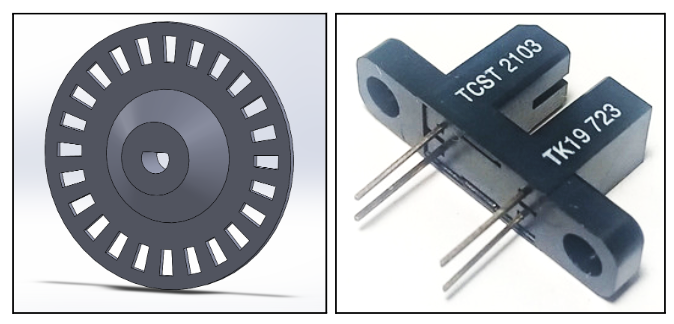
\includegraphics[width=0.7\linewidth]{images/encoder.png}
  \caption{Modelo 3D del encoder rotativo y opto acoplador de ranura}
  \label{fig:encoder}
\end{figure}

Por último se debe destacar que es necesario filtrar el rebote de los flancos de subida y bajada en cada interrupción.

\subsubsection{Elección de lenguaje para interfaz} \mbox{} \vspace{10pt} \\
En cuanto a las elección del lenguaje se refiere, teníamos dos caminos para elegir, ya que nos encontrábamos limitados por el microcontrolador que soporta tanto C como microPython. Habiendo hecho un análisis y una lectura de las distintas APIs que el fabricante nos ofrece, optamos por C ya que es un lenguaje conocido por nosotros. Esto porque durante el transcurso de la carrera nos tocó desarrollar varios trabajos prácticos en este lenguaje, por lo que sentíamos que no necesitabamos adquirir muchos nuevos conocimientos, es un entorno cómodo para trabajar y la documentación es que se encuentra es amplia por lo que los problemas que podían llegar a surgir los íbamos a poder sortear con cierta facilidad.
En el escenario de seguimiento del robot nos encontramos con el desafió de realizar una interfaz amigable, entendible y que pueda desarrollarse de la forma mas rápida posible sin la necesidad de tener una curva de aprendizaje muy grande. Es por ello que optamos por Python para poder cumplir todos los requisitos ya mencionados. Ambos integrantes ya habíamos trabajado con este lenguaje, y ademas, últimamente, se lo encuentra seguido entre los lenguajes mas utilizados por toda la comunidad de la programación, esto por ser un lenguaje sumamente adaptable ante cualquier necesidad y contar con una variedad muy extensa de librerías. Nos pareció una buena elección que nos daba la opción de sortear cualquier obstáculo que surgiera en el camino.

\subsubsection{Comunicación inalámbrica}

Nuestro proyecto al estar pensado para cumplir con los estándares de la Industria 4.0, nos vimos en la necesidad de incorporar la comunicación inalámbrica como medio principal para poder conectar y establecer comunicación entre los distintos componentes que forman parte del proyecto. Así como muestra el diagrama de alto nivel, los componentes se comunican utilizando un router como medio para poder llegar uno hacia otro.

Los microcontroladores elegidos vienen incorporados con los integrados necesarios para hacer uso de esta tecnología y ademas cuentan con la posibilidad de incorporarles una antena, lo que mejora la calidad de la señal y amplia su rango de alcance por lo que los vuelve mas efectivos aun si es que se necesita enviar gran cantidad de información y asegurar que los paquetes van a llegar a destino.

Existe la posibilidad de usar protocolos propios de estos microcontroladores, como ser ESP-NOW, para establecer una comunicación mas segura entre los microcontroladores, pero, optamos por hacer uso del protocolo MQTT que es usado ampliamente en la industria para enviar información de sensores y mensajes cortos. Esto debido a la liviandad y eficiencia de sus mensajes, además, de no atarnos por completo a un protocolo privativo de la marca ESP y poder usar lo que hasta ahora viene siendo un estándar para los dispositivos IoT.

\begin{figure}[H]
   \centering
   
\includegraphics[width=0.7\linewidth]{images/com_inalambrica.jpg}
   \caption{Protocolos usados comúnmente en entornos IoT}
   \label{fig:mqtt}
\end{figure}

\subsection{Testing y pruebas}

Las pruebas que se realizaron para que efectivamente podamos determinar el correcto funcionamiento del Monitor, la gestión de la cola de cortesía y la resolución de conflictos mediante la aplicación de una Política fue con la ayuda de la Red de Petri sumamente conocida como Productor-Consumidor. Esta se tomó cómo referencia ya que permite evaluar los problemas de sincronización, concurrencia y gestión de los recursos, entonces, nos pareció un buen puntapié para validar el funcionamiento con un modelo conocido y sumamente usado. Cabe destacar que realizamos la simulación sobre esta red alrededor de $1M$ de disparos y por supuesto siempre validando el resultado de los $P\ invariantes$ y $T\ invariantes$.

\begin{figure}[H]
   \centering
   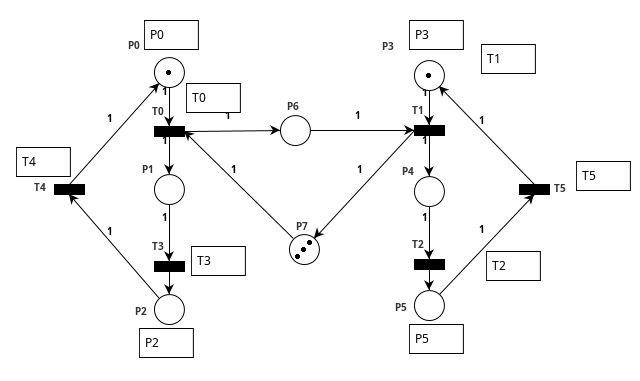
\includegraphics[width=0.9\linewidth]{images/rdp_prod_cons.png}
   \caption{Red de Petri productor-consumidor}
   \label{fig:rdp_prod_cons}
\end{figure}

Se plantearon los siguientes casos:

\begin{testtableformat}
   \hline \rowcolor{test_header_color}
       Test ID             & TC\_04\_00 \\
   \hline
       Tipo de test        & Test unitario \\
   \hline
       Objeto de prueba    & Disparar las transiciones sensibilizadas del Productor \\
   \hline
       Nombre              & Ejecución del productor \\
   \hline
       Descripción         & Realizar el disparo de las transiciones sensibilizadas del productor teniendo como máximo 3 (tres) tokens disponibles para producir\\
   \hline
       Precondición        & PRECOND\_D \\
   \hline
       Pasos del test      & \begin{enumerate}
                             \item Instanciar a la clase monitor con la red productor-consumidor
                             \item Obtener el vector de transiciones sensibilizadas 
                             \item Ejecutar un disparo de la transición sensibilizada 
                             \item Adquirir el marcado saliente y compararlo con un programa de análisis de redes de Petri 
                             \end{enumerate}\\
   \hline
       Resultado esperado  & El marcado en ambos casos debe coincidir \\
   \hline
       Resultado obtenido  & El marcado de la red obtenido por la clase monitor y el programa de análisis de redes de Petri son iguales, por lo tanto, se verifica su adecuado funcionamiento \\
   \hline
       Observaciones       & -\\
   \hline
\end{testtableformat}

\begin{testtableformat}
   \hline \rowcolor{test_header_color}
       Test ID             & TC\_04\_01 \\
   \hline
       Tipo de test        & Test unitario \\
   \hline
       Objeto de prueba    & Disparar las transiciones sensibilizadas del consumidor \\
   \hline
       Nombre              & Ejecución del consumidor \\
   \hline
       Descripción         & Realizar el disparo de las transiciones sensibilizadas del consumidor teniendo como máximo 3 (tres) recursos disponibles generados por el productor\\
   \hline
       Precondición        & PRECOND\_D \\
   \hline
       Pasos del test      & \begin{enumerate} 
                             \item Instanciar a la clase monitor con la red productor-consumidor 
                             \item Obtener el vector de transiciones sensibilizadas 
                             \item Ejecutar un disparo de la transición sensibilizada 
                             \item Adquirir el marcado saliente y compararlo con un programa de analisis de redes de petri 
                             \end{enumerate}\\
   \hline
       Resultado esperado  & El marcado en ambos casos debe coincidir \\
   \hline
       Resultado obtenido  & El marcado de la red obtenido por la clase monitor y el programa de análisis de redes de Petri son iguales, por lo tanto, se verifica su adecuado funcionamiento \\
   \hline
       Observaciones       & -\\
   \hline
\end{testtableformat}

\begin{testtableformat}
   \hline \rowcolor{test_header_color}
       Test ID             & TC\_04\_02 \\
   \hline
       Tipo de test        & Test unitario \\
   \hline
       Objeto de prueba    & Disparar una transición con política de decisión \\
   \hline
       Nombre              & Ejecución de una transición con política definida \\
   \hline
       Descripción         & En en el caso donde tanto el productor cómo el consumidor pueden disparar una transición, la idea es evaluar la política de la transición del consumidor para que tenga prevalencia sobre el productor ante una situación indeterminista \\
   \hline
       Precondición        & PRECOND\_E \\
   \hline
       Pasos del test      & \begin{enumerate} 
                             \item Instanciar a la clase monitor con la red productor-consumidor 
                             \item Generar una situación de equidad donde ambos recursos puedan disparar su transición 
                             \item Obtener el vector de transiciones sensibilizadas 
                             \item Evaluar la política de las transiciones sensibilizada y elegir cual disparar 
                             \item Ejecutar un disparo de la transición elegida 
                             \item Adquirir el marcado saliente y compararlo con un programa de análisis de redes de petri 
                             \end{enumerate}\\
   \hline
       Resultado esperado  & El marcado actual en ambos casos debe coincidir y la transición disparada debe ser la del consumidor \\
   \hline
       Resultado obtenido  & El marcado de la red obtenido por la clase monitor y el programa de análisis de redes de Petri son iguales, por lo tanto, se verifica su adecuado funcionamiento \\
   \hline
       Observaciones       & -\\
   \hline
\end{testtableformat}

\begin{testtableformat}
   \hline \rowcolor{test_header_color}
       Test ID             & TC\_04\_03 \\
   \hline
       Tipo de test        & Test integración \\
   \hline
       Objeto de prueba    & Realizar movimientos con el robot dentro del mapa, el robot sólo va a avanzar cuando la red de Petri haya hecho la solicitud de disparo y haya verificado que el robot no se encuentra bloqueado.\\
   \hline
       Nombre              & Desplazamientos del robot controlado por el Monitor\\
   \hline
       Descripción         & Para que el robot avance de una celda a otra y realice el desplazamiento definido (punto inicial y final) debe ser autorizado y coordinado por el monitor que controla la red de Petri.\\
   \hline
       Precondición        & PRECOND\_E \\
   \hline
       Pasos del test      & \begin{enumerate}
                             \item Indicar los puntos de inicio y final del robot
                             \item Esperar que el Monitor dispare la transición sensibilizada
                             \item El robot recibe la orden de avanzar a la celda libera
                             \item El robot envía una señal de llegada a la celda (plaza)
                             \item Se dispara la siguiente transición sensibilizada
                             \item Este proceso se repite hasta que el robot llegue a su destino
                             \end{enumerate}\\
   \hline
       Resultado esperado  & El robot pueda completar su desplazamiento definido por el usuario\\
   \hline
       Resultado obtenido  & La red de Petri al no bloquearse permite que todas las transiciones sensibilizadas se puedan disparar y por ende que el robot pueda desplazarse por todas las celdas (plazas) involucradas en su recorrido\\
   \hline
       Observaciones       & -\\
   \hline
\end{testtableformat}

\begin{testtableformat}
    \hline \rowcolor{test_header_color}
        Test ID             & TC\_04\_04 \\
    \hline
        Tipo de test        & Test de sistema \\
    \hline
        Objeto de prueba    & Comunicación inalámbrica - PID - Modelo cinemático - Odometría - Seguidor de línea magnética - Modelo del mapa - Calculador de trayectorias - Interfaz de usuario - Red de Petri - Monitor \\
    \hline
        Requerimiento       & RF1 - RF2 - RF3 - RF4 - RF5 - RF6 - RF7 - RF10 \\
    \hline
        Nombre              & Prueba de sistema integrado\\
    \hline
        Descripción         & Comprobar que el robot se puede desplazar por el mapa gestionado por el marcado de la red de Petri\\
    \hline
        Precondición        & PRECOND\_G \\
    \hline
        Pasos del test      & \begin{enumerate}
                              \item Indicar los puntos de inicio y final del robot en el mapa
                              \item Calcular la secuencia de disparos del Monitor
                              \item Esperar que el Monitor dispare la transición sensibilizada
                              \item El robot recibe la orden de avanzar a la celda (plaza) liberada
                              \item El robot envía una señal de llegada a la celda (plaza) destino
                              \item Se dispara la siguiente transición sensibilizada
                              \item Este proceso se repite hasta que el robot llegue a su destino
                              \end{enumerate}\\
    \hline
        Resultado esperado  & El robot pueda completar su desplazamiento definido por el usuario\\
    \hline
        Resultado obtenido  & La red de Petri al no bloquearse permite que todas las transiciones sensibilizadas se puedan disparar y por ende que el robot pueda desplazarse por todas las celdas (plazas) involucradas en su recorrido\\
    \hline
        Observaciones       & Se probó recorridos de 4 de metros por limitaciones de espacio\\
    \hline
 \end{testtableformat}

\subsection{Resultados}
El resultado es satisfactorio debido a que pudimos recolectar gran cantidad de información de todos los componentes y armamos el principio de lo que será el desarrollo de todo el proyecto.

\subsection{Riesgos superados}
\begin{center}
    \begin{tabular} {
        | c| c |}
        \hline \rowcolor{test_header_color}
            ID & Riesgo \\
        \hline
            RI-04 & Modificación de los requerimientos del proyecto\\
        \hline
    \end{tabular}
\end{center}

\subsection{Conclusiones}
En base a los información recolectada y leída, vemos que planteamos una base por donde comenzar el proyecto, definiendo los sistemas y componentes que se van a usar para su implementación, por lo tanto nos sentimos cómodos con las decisiones tomadas y vemos con buenos ojos el comienzo del desarrollo.

\newpage
\section{Iteración 1: Prototipo del robot}

\subsection{Introducción}
En la iteración anterior obtuvimos como resultado los principios y bases fundamentales sobre las que desarrollaremos esta iteración para lograr un prototipo funcional.

\subsection{Requerimientos}
En esta iteración abordaremos los siguientes requerimientos funcionales:

\begin{center}
\begin{tabular}{
    | >{\centering\arraybackslash}m{1cm}
    | >{\centering\arraybackslash}m{13cm} |
}
\hline \rowcolor{test_header_color}
    ID & Descripción \\
\hline
    RF1 & El robot debe contar con un sistema de control para las 4 ruedas. \\ 
\hline
    RF2 & El robot debe tener un sistema de locomoción omnidireccional. \\ 
\hline
    RF3 & El robot debe poder medir la distancia recorrida. \\ 
\hline
    RF4 & El robot debe poder realizar trayectorias en línea recta y curvas. \\ 
\hline
    RF5 & El robot debe poder corregir su trayectoria mediante el uso de sensores. \\  
\hline
    RF6 & El robot debe recibir y enviar información mediante comunicaciones inalámbricas. \\ 
\hline
\end{tabular}
\end{center}

Por otra parte, los requerimientos no funcionales que trataremos son:

\begin{center}
\begin{tabular}{
    | >{\centering\arraybackslash}m{1cm}
    | >{\centering\arraybackslash}m{13cm} |
}
\hline \rowcolor{test_header_color}
    ID & Descripción \\
\hline
    RNF1 & Debería tener tiempos de respuesta aceptables para el buen funcionamiento del sistema de control. \\
\hline
    RNF2 & El software debería contar con pruebas unitarias y de integración. \\
\hline
    RNF4 & El código debería contar con documentación.\\
\hline
\end{tabular}
\end{center}

\subsection{Desarrollo}

\subsubsection{Sistema de control PID}
Un controlador PID (Proporcional-Integral-Derivativo) es un tipo de controlador utilizado en sistemas de control automático para mantener una variable de algún proceso lo más cercana posible a un valor deseado, conocido como "setpoint", a pesar de las perturbaciones encontradas. La acción proporcional responde al error actual, que es la diferencia entre el valor deseado y el valor medido, ajustando la salida del controlador proporcionalmente a este error. Por otro lado, la acción integral se enfoca en la acumulación de errores pasados para eliminar cualquier error que sea persistente, asegurando que con el tiempo la variable de proceso converja al setpoint establecido. Finalmente, la acción derivativa considera la tasa de cambio del error, anticipando y corrigiendo cualquier futura tendencia del error, sumando a la estabilidad del sistema.

El objetivo principal de un controlador PID es proporcionar una respuesta rápida y estable en diferentes aplicaciones. Además de ser utilizado en procesos industriales como plantas químicas y refinerías, también se lo utiliza en el control de velocidad de motores eléctricos, asegurando que el motor funcione a la velocidad deseada sin fluctuaciones por mas que se perciban alteraciones, por lo que en robótica resultan útiles para el control de posición y movimiento, permitiendo acciones precisas y controladas.

\paragraph{Función de transferencia del motor} \mbox{} \vspace{8pt}

La función de transferencia en un sistema de control se representa como $G(s)$ y modela matemáticamente el comportamiento de un actuador, al cual se le aplica un estimulo o señal $R(s)$ y se obtiene una respuesta $C(s)$ por parte de él.

Para controlar la variable en cuestión debemos tener una noción sobre la salida producida. Por un lado tenemos la función $H(s)$, que es una función que toma como entrada una medición sobre la salida del actuador o sistema para producir un valor $B(s)$. Éste se suma negativamente al setpoint $R(s)$ para obtener el error entre ellas $E(s)$, que es la señal efectivamente que se introduce a $G(s)$ para logar aproximarse al setpoint y compensar el sistema.

\begin{figure}[H]
    \centering
    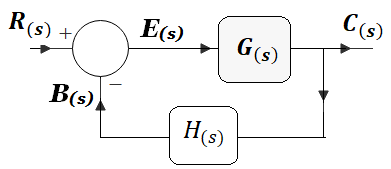
\includegraphics[width=0.4\linewidth]{sistema_de_control}
    \caption{Sistema de control realimentado}
    \label{fig:sistcontrolrealim}
\end{figure}

Para lograr controlar cada motor de cada rueda es necesario conocer la función de transferencia del mismo para lograr modelarlo. Al no contar con la hoja de datos del fabricante por ser un motor genérico, se realizaron una serie de experimentos para aproximar la función $G(s)$. En nuestro caso debemos obtener una función de transferencia que tenga como entrada $[Volts]$ y su salida sea $[RPM]$.

Para hacer esto se propone hacer uso del método de la constante de tiempo $\tau$. En primer lugar, consideraremos que la curva alcanza el $63.2\%$  del valor final cuando ha transcurrido un tiempo $t=\tau$. En la gráfica el valor final de la curva es 1, es decir, $y(\infty)=1$. Por lo que debemos identificar el instante $t$ para el cual se cumple que $y(t)=0.632$.

El paso siguiente es trazar una recta paralela al eje de las abscisas (eje $t$) que corresponda al $63.2\%$ del valor final de $y(t)$. Desde ese punto, se traza una recta paralela al eje de las ordenadas (eje $y$) hasta cortar el eje $t$. Este punto de intersección corresponde al valor de $\tau$.

\begin{figure}[H]
    \centering
    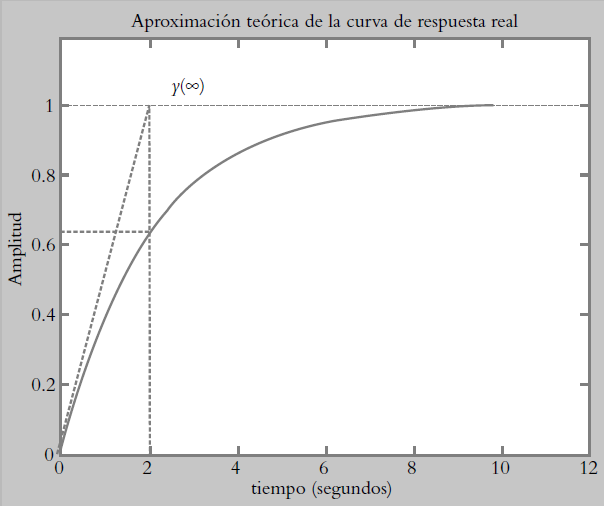
\includegraphics[width=0.625\linewidth]{metodo_const_tiempo_func_transf}
    \caption{Método de la constante de tiempo}
    \label{fig:metodoctetiempo}
\end{figure}

Obtenido esto, se procede a elaborar un sistema de primer orden mediante la siguiente expresión:

$$ G(s) = \frac{k}{\tau \cdot s + 1} $$

Donde $k$ representa la ganancia estática, que es el valor al que tiende la salida del sistema cuando la entrada es una señal constante y el tiempo tiende a infinito. En otras palabras, es el factor de escala entre la entrada y la salida en estado estacionario.

Para identificar la ganancia estática $k$, partimos de que en estado estacionario la salida alcanza un valor constante $y(\infty)$. Además, se considera que estimulamos al actuador con una señal escalón, denominada $u(\infty)$. La ganancia estática se puede calcular como:

$$ k=\frac{y(\infty)}{u(\infty)} $$

Para medir la respuesta del motor, primero conectamos mecánicamente el eje del motorreductor a medir junto con el eje de otro motor testigo, el cual esta conectado a un osciloscopio. Con esta experiencia buscamos estimular al motorreductor con una señal escalón unitario y que el motor testigo genere una tensión que se puede registrar en el osciloscopio. De este modo obtuvimos los valores de tensión generada en el motor testigo y podemos estimar la respuesta del motorreductor. En la Figura \ref{fig:exprespmotor} se muestra un diagrama de la experiencia.

\begin{figure}[H]
    \centering
    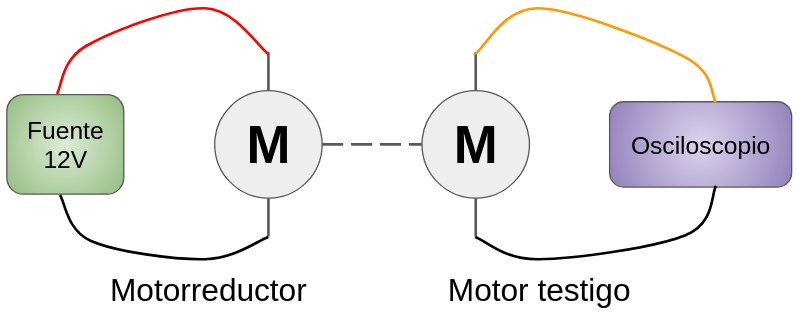
\includegraphics[width=0.55\linewidth]{experim_resp_motor}
    \caption{Experiencia para medición de RPM}
    \label{fig:exprespmotor}
\end{figure}

En el osciloscopio logramos obtener la gráfica que se muestra en la Figura \ref{fig:curvarespmotor}. En amarillo se representa la entrada escalón de 12V hacia el motor y en verde la tensión generada en el motor testigo.

\begin{figure}[H]
    \centering
    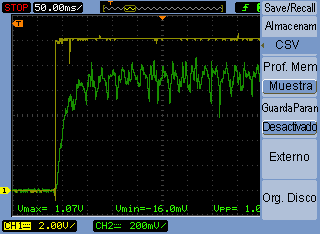
\includegraphics[width=0.525\linewidth]{curva_resp_motor_osciloscopio}
    \caption{Curva de respuesta del motorreductor}
    \label{fig:curvarespmotor}
\end{figure}

Luego procedimos a extraer los puntos de datos y suavizar la curva para facilitar el análisis. Esto lo hicimos mediante una media ponderada con un factor $\alpha = 0.2$, obtenido experimentalmente:

$$ S_{t} = \alpha \cdot Y_{t-1} + (1 - \alpha) \cdot Y_{t} $$

A partir de ello obtuvimos la gráfica de la Figura \ref{fig:curvarespmotorsuaviz}, donde en el eje horizontal están representados instantes de tiempo equivalentes a $10[ms]$ cada uno y en el eje vertical el voltaje (expresado en $[volts]$) sensado en el motor testigo.

Ahora bien, para linealizar el sistema podemos suponer que el valor de tensión generado en el motor testigo es proporcional a las revoluciones por minuto que gira su eje. Dado que en la iteración anterior se logró la implementación de un medidor de RPM, obtuvimos en este caso que el motorreductor conectado a 12V continuos produce 92 [RPM]. En este momento podemos calcular la ganancia estática $k$:

$$ k=\frac{y(\infty)}{u(\infty)}=\frac{92[RPM]}{12[V]}=7.66[RPM/V] $$

\begin{figure}[H]
    \centering
    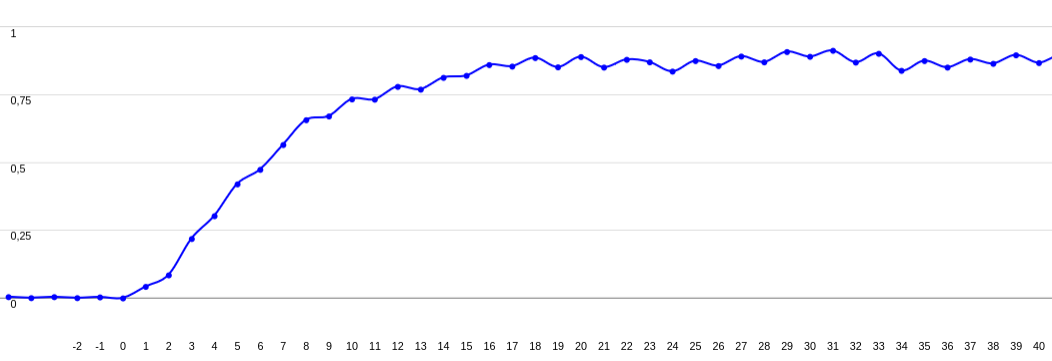
\includegraphics[width=1.0\linewidth]{resp_motor_suavizado}
    \caption{Curva de respuesta del motor suavizada}
    \label{fig:curvarespmotorsuaviz}
\end{figure}

Por otra parte, determinamos que $\tau=70[ms]$ por alcanzar en esa marca el valor de tensión $0,564[V]$, rondando el $63.2\%$ del valor en estado estacionario. Aplicando la expresión para obtener un sistema de primer orden obtenemos:

$$ G(s) = \frac{7.66}{0.07 \cdot s + 1} $$

% https://dademuchconnection.wordpress.com/2021/06/26/aproximacion-teorica-de-una-curva-de-respuesta-real/
% https://controlautomaticoeducacion.com/control-realimentado/ziegler-nichols-sintonia-de-control-pid/

\paragraph{Diseño del controlador} \mbox{} \vspace{8pt}

Es tarea del controlador intervenir para corregir las fluctuaciones que sufre el sistema. Por lo general los controladores PID basan su funcionamiento en 3 parámetros fundamentales, los cuales son $K_p$, $K_i$ y $K_d$; correspondiéndose con el factor de acción proporcional, integrativa y derivativa, respectivamente.

En nuestro caso, optamos por utilizar un PID aditivo por ser de sencilla implementación y por ser mas rápida la convergencia a los coeficientes óptimos. En la Figura \ref{fig:pidaditivo} se muestra un diagrama del mismo.

\begin{figure}[H]
    \centering
    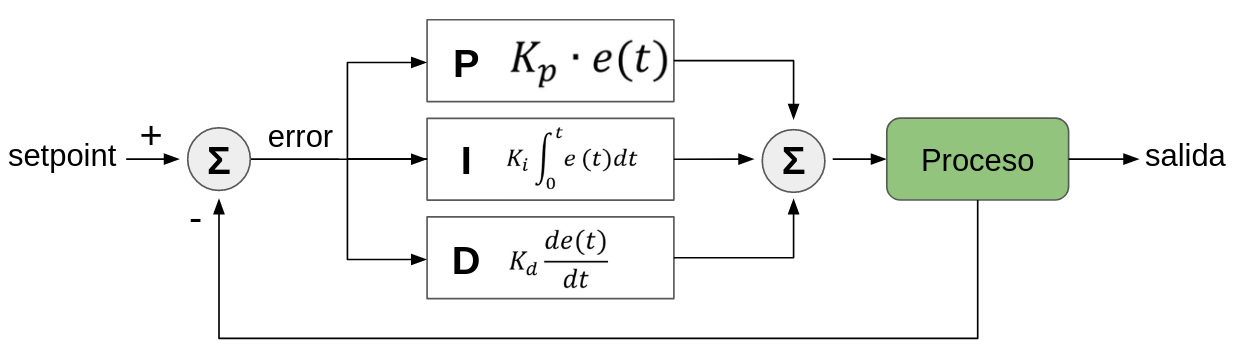
\includegraphics[width=1.0\linewidth]{images/pid_aditivo}
    \caption{PID aditivo}
    \label{fig:pidaditivo}
\end{figure}

\paragraph{Implementación} \mbox{} \vspace{8pt}

Cada uno de los cuatro motores del robot tiene su propio controlador PID, todos con coeficientes idénticos. Se implementan dentro del microcontrolador ESP32 haciendo uso de los puertos de salida PWM para controlar la velocidad y sentido de cada una de las ruedas. Además se utilizan los módulos contadores de pulsos asociados a los puertos GPIO donde se conecta cada encoder rotativo.

Como requerimiento, debe contar con tiempos de respuesta aceptables para que el sistema de control funcione adecuadamente, por lo que hicimos pruebas para descubrir el mejor $\Delta T$ de actualización del PID, en concordancia con el período de medición de RPM. Pudimos determinar que el controlador cumple con el requerimiento teniendo un periodo mínimo de $T=100[ms]$.

Por cada motor se tiene una estructura como la siguiente:

\begin{figure}[H]
    \centering
    \hspace*{-0.75cm}
    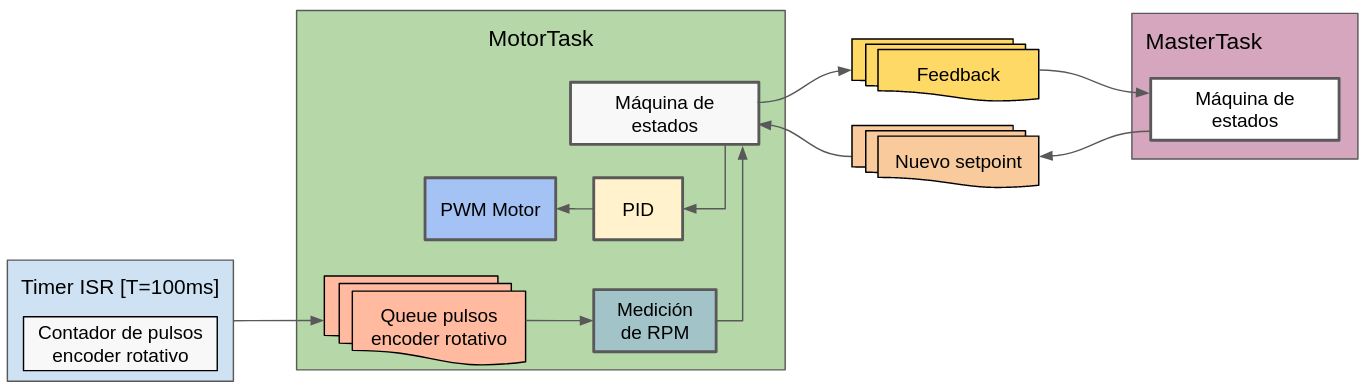
\includegraphics[width=1.1\linewidth]{images/diag_comp_esp32_pid_solo.png}
    \caption{Diagrama de componentes del firmware de la ESP32}
    \label{fig:diagcomponentesp32}
\end{figure}

En primer lugar, se tiene una interrupción periódica de $T=100[ms]$ donde se toman los valores de cada uno de los módulos contadores de pulso (PCNT) del microcontrolador, vinculados a los encoders rotativos de cada rueda. Existe una cola por cada MotorTask para recibir esta información desde la interrupción. Por otro lado, la tarea MasterTask cuenta con una cola (queue) única que comparte con todas las MotorTask para recibir el feedback de las mismas. Asimismo, cada tarea MotorTask tiene una cola que comparte con la tarea MasterTask, donde se envía un setpoint independiente a cada rueda.

Al ser el robot omnidireccional, si se establecen todas las ruedas a la misma velocidad y en sentidos determinados, es posible lograr que el robot de mueva a lo largo de un vector en linea recta sobre el plano. De este modo podemos llevar a cabo pruebas con las que encontramos los coeficientes del controlador.

A continuación, incurrimos en la utilización de la técnica de Ziegler-Nichols a lazo abierto y logramos obtener valores aproximados de $K_p$, $K_i$ y $K_d$. Introdujimos estos valores en el controlador y colocamos el robot en el suelo para realizar una serie de pruebas en línea recta. Con estos coeficientes no notamos un comportamiento óptimo, por lo que nos enfocamos en iterar sobre los valores y ajustar las constantes.

De este modo se realizaron iteraciones aumentando o disminuyendo cada uno de los coeficientes para buscar el punto óptimo de funcionamiento. Comenzamos con un valor de $K_p=10$ y un setpoint de $65[RPM]$, los demás coeficientes en cero. De este modo se fue aproximando el valor hasta lograr un arranque rápido pero sin demasiado sobrepaso. Una vez obtenido lo anterior, se procedió a ajustar $K_i$ observando cómo variaba el error acumulado al alcanzar las RPM deseadas. Para finalizar, se determinó el factor $K_d$ mediante observación de la respuesta del robot ante picos de perturbaciones.

Finalmente, obtenemos la siguiente estructura para el control de las 4 ruedas independientes del robot:

\begin{figure}[H]
    \centering
    \hspace*{-0.75cm}
    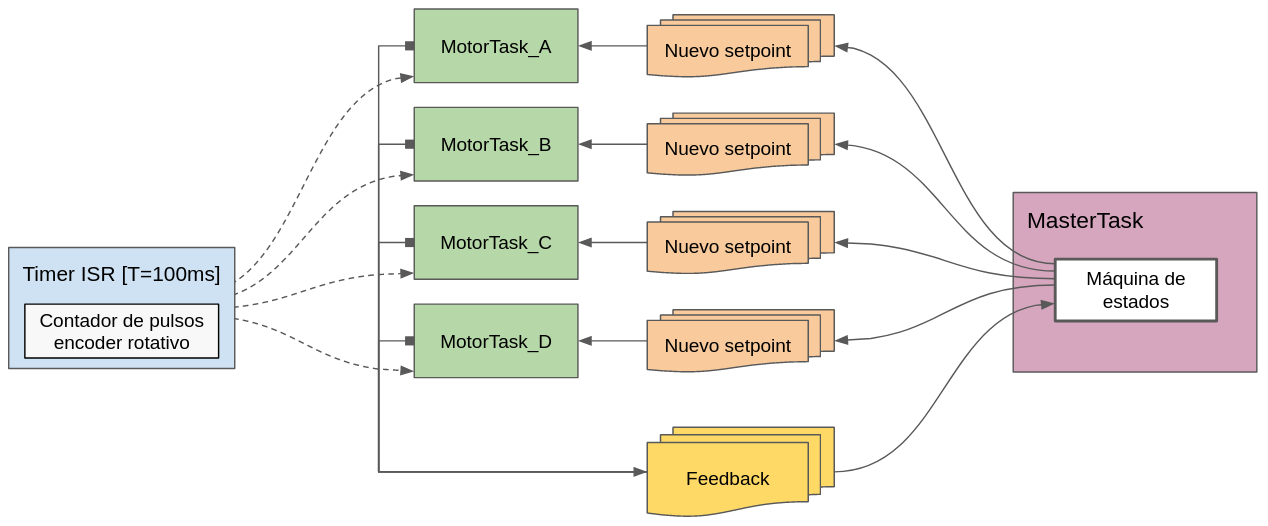
\includegraphics[width=1.05\linewidth]{images/diag_comp_esp32_pid_solo_todos_los_motores.png}
    \caption{Estructura de control de los motores}
    \label{fig:diagcommpesp32pidmotores}
\end{figure}

A continuación se detalla el funcionamiento de una de las tareas de los motores con la tarea principal. El proceso es similar para las demás MotorTask.

\begin{figure}[H]
    \centering
    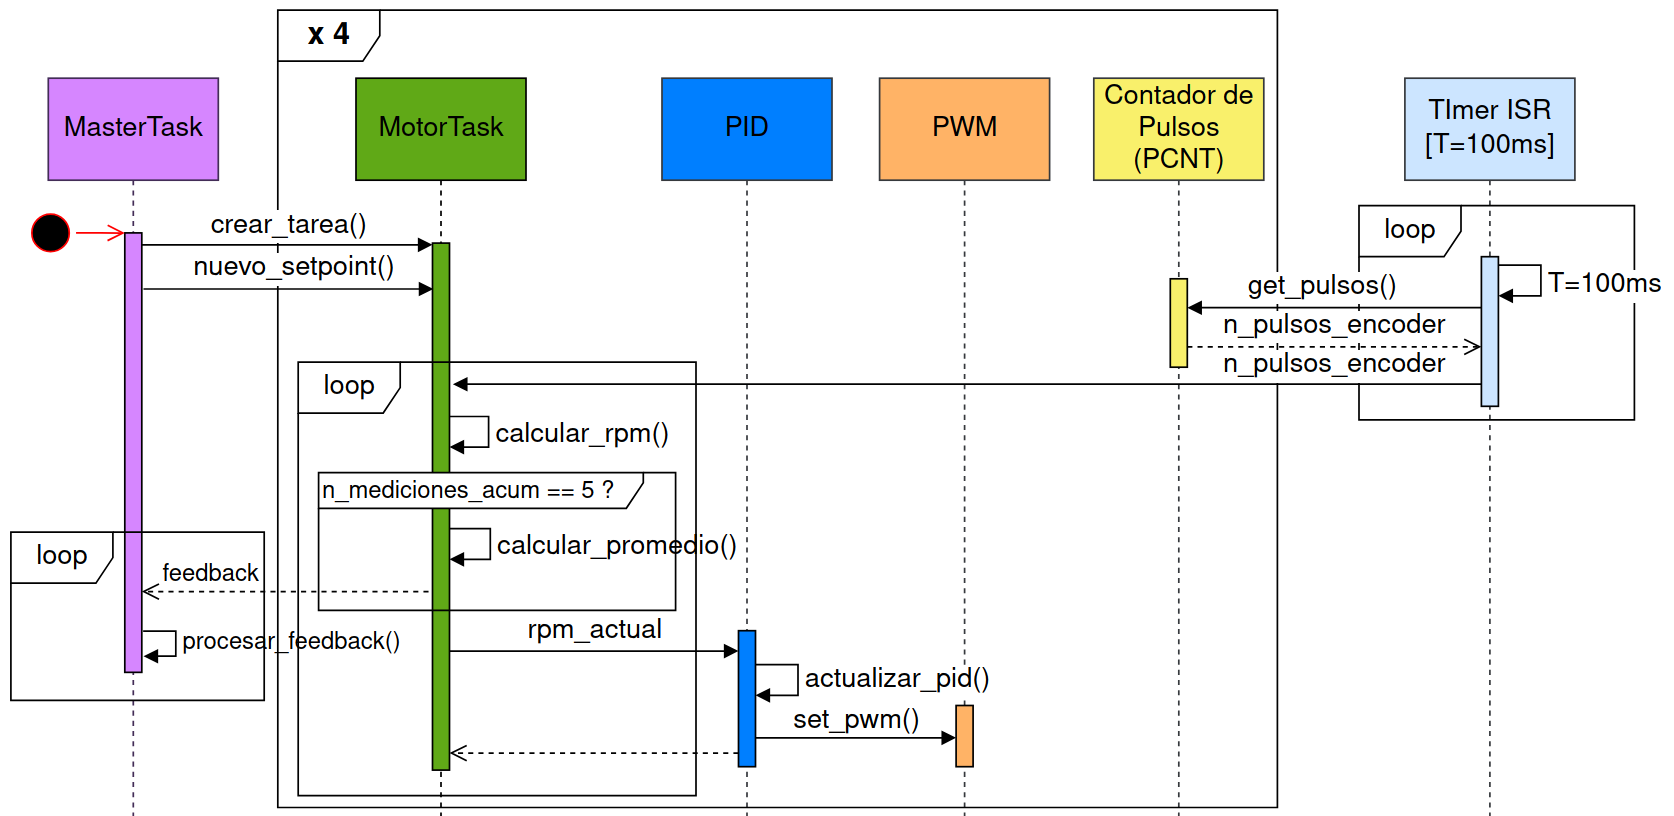
\includegraphics[width=1.1\linewidth]{images/diag_secuencia_pid_solo.png}
    \caption{Diagrama de secuencia de las tareas de control para los motores}
    \label{fig:diagsecuenciapidsolo}
\end{figure}


% fuentes de esta seccion 
% https://www.mdpi.com/2076-3417/12/5/2606
% https://tesis.ipn.mx/jspui/bitstream/123456789/18688/1/Sistema%20de%20control%20para%20el%20desplazamiento%20omnidireccional%20de%20un%20robot%20m%C3%B3vil.pdf


\subsubsection{Modelo cinemático}

La cinemática se define como la ciencia que estudia el movimiento de objetos sin tomar en cuenta sus inercias. Dentro de la misma se estudia la posición, la velocidad, la aceleración y todas las demás derivadas de alto orden de las variables de posición con respecto al tiempo.

Para lograr representar matemáticamente al robot se utilizan ecuaciones que relacionan las velocidades de las ruedas con la velocidad lineal y angular del robot en el plano. Estas ecuaciones se derivan de la disposición geométrica de las ruedas y las características de las ruedas omnidireccionales. Utilizando matrices de transformación, es posible describir cómo las velocidades de las ruedas se combinan para producir el movimiento deseado del robot. Para ello se definen dos elementos fundamentales, la ecuación cinemática directa y la ecuación cinemática inversa. \cite{tzafestas2013introduction}

En el contexto de un robot omnidireccional de 4 ruedas, la cinemática directa permite traducir un vector de movimiento lineal del robot en velocidades específicas para cada rueda independiente. Cada rueda se mueve independientemente y por su configuración, permite que el robot se pueda desplazar lateralmente, hacia adelante, hacia atrás, gire sobre su propio eje y realice trayectorias curvas. \cite{rijalusalamkinematics}

Es importante que tengamos en cuenta que para tener un sistema de control acotado y predecible, es necesario compensarlo de algún modo. En este caso debemos ser capaces de obtener el vector de movimiento del robot en base a las velocidades angulares medidas en las ruedas y así lograr detectar diferencias con el vector de movimiento deseado. Para ello nos resulta útil la cinemática inversa, que implica medir las velocidades angulares de cada una de las cuatro ruedas para obtener el vector de movimiento que el robot realiza. Esto es crucial para el control y navegación del robot dado que corrige las alteraciones de un entorno dinámico.

El desarrollo de estas ecuaciones implica calcular cómo las velocidades de cada rueda contribuyen al movimiento global del robot y cómo se deben ajustar estas velocidades para lograr una trayectoria específica. En otras palabras, estas ecuaciones toman en cuenta la disposición y orientación de las ruedas y cómo contribuyen al movimiento global del robot, aprovechando al máximo la capacidad omnidireccional del robot.

Una vez logrado un modelo cinemático que aproxime bien el sistema real, deberíamos poder establecer un vector de movimiento deseado y obtener la velocidad a la que se debe colocar cada rueda para poder transcurrirlo. No solo debería poder hacer movimientos rectos en cualquier dirección, sino que también sería capaz de hacer movimientos rotatorios con traslación sobre el plano, formando trayectorias elípticas. \cite{rijalusalamkinematics}

En nuestro caso se trata de un robot cuadrado con 1 rueda por cada lado cuya orientación respecto al robot es fija. Ademas de ello, se utilizan ruedas de tipo Omni-wheel, las cuales son similares a las ruedas Mecanum. Son ruedas que cuentan con pequeños discos (llamados rodillos) alrededor de la circunferencia perpendiculares a la dirección de giro. El efecto es que la rueda puede moverse con toda su fuerza, pero también se deslizará lateralmente con gran facilidad.

\begin{figure}[H]
    \centering
    \includegraphics[width=0.3\linewidth]{omni-wheel-wikipedia}
    \caption{Rueda omnidireccional Omni-Wheel}
    \label{fig:ruedaomniwheel}
\end{figure}

Teniendo en cuenta lo anterior, para la construcción del modelo cinemático se consideran las siguientes limitaciones:

\begin{itemize}
    \item El robot se mueve sobre una superficie plana lisa.
    \item No existen elementos flexibles en la estructura del robot.
    \item El eje de direccionamiento de las ruedas siempre es perpendicular al suelo.
    \item No se consideran ningún tipo de fricciones contra el suelo.
\end{itemize}

\paragraph{Desarrollo} \mbox{} \vspace{8pt}

Al suponerse la rueda como un elemento rígido, se establece el principio de que las ruedas en contacto con el suelo se comportan como una articulación planar de tres grados de libertad, con lo que se propone el sistema de referencia descrito en la siguiente figura:

\begin{figure}[H]
    \centering
    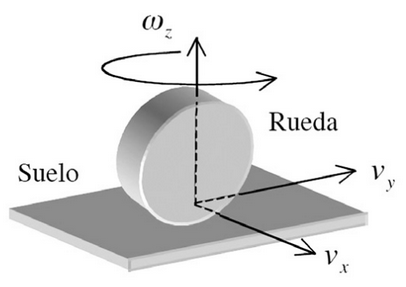
\includegraphics[width=0.4\linewidth]{rueda_modelo_cinematico}
    \caption{Vectores actuantes en una rueda}
    \label{fig:vectoresrueda}
\end{figure}

El eje $V_y$ determina el sentido normal de avance de la rueda, el eje $V_x$ indica los desplazamientos laterales y $\omega_z$ la velocidad rotacional que se produce cuando el vehículo realiza un giro.

Definimos al robot sobre el plano cartesiano, donde se establece el marco de referencia global representado por $oxy$ y el marco de referencia local del robot $o_rx_ry_r$, donde el marco de referencia local se encuentra alineado con el marco de referencia global.

\begin{figure}[H]
    \centering
    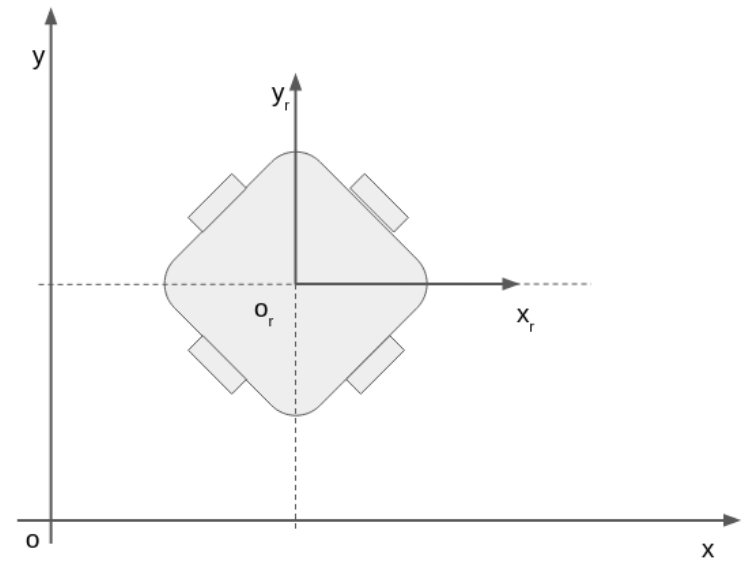
\includegraphics[width=0.6\linewidth]{robot_en_el_plano_mod_cinem}
    \caption{Marco de referencia del robot y del espacio}
    \label{fig:marcorefrobotenelplano}
\end{figure}

Además podemos representar el robot y la distribución de ruedas del siguiente modo:

\begin{figure}[H]
    \centering
    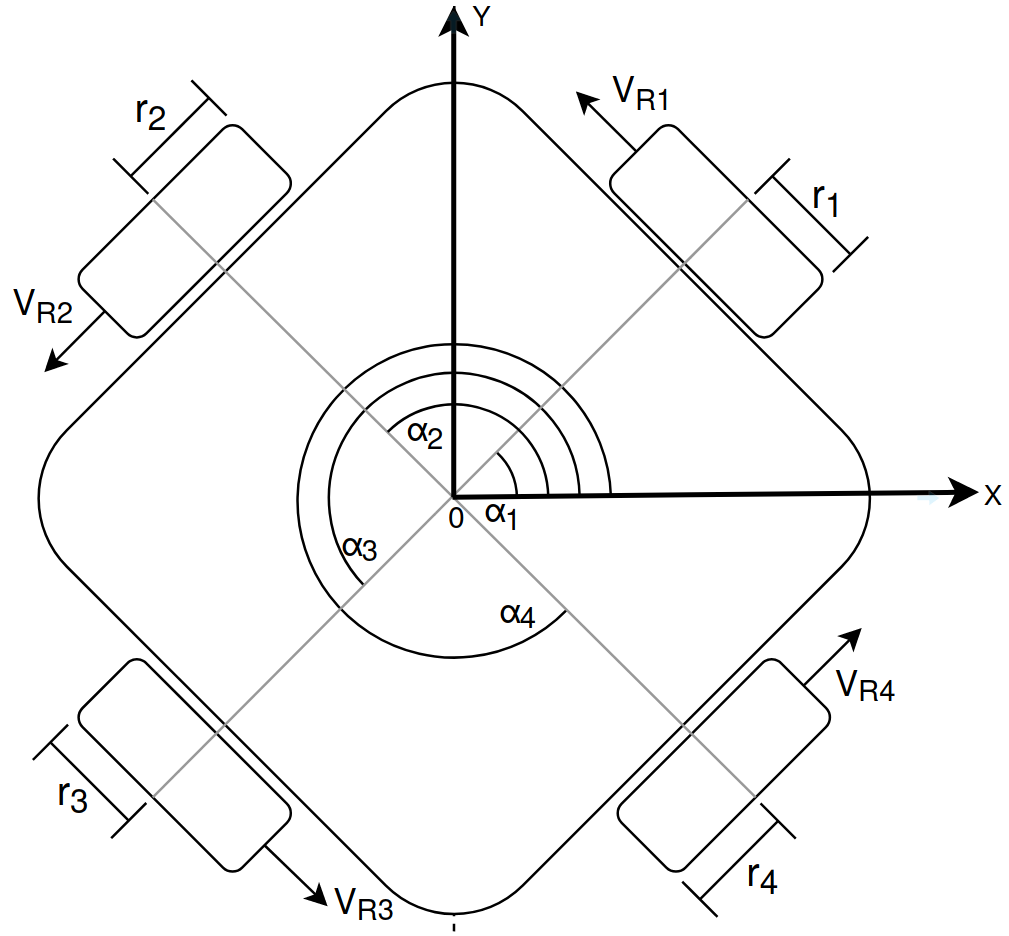
\includegraphics[width=0.6\linewidth]{images/modelo_cinematico_robot_ruedas.png}
    \caption{Descomposición de vectores del robot}
    \label{fig:vectoresrobotmodelocinem}
\end{figure}

Se establece que el angulo entre las ruedas y el cuerpo del robot es fijo y está dado por:

$$ \alpha_1 = \frac{\pi}{4} = 45^{\circ} $$
$$ \alpha_2 = \frac{3\pi}{4} = 135^{\circ} $$
$$ \alpha_3 = \frac{5\pi}{4} = 225^{\circ} $$
$$ \alpha_4 = \frac{7\pi}{4} = 315^{\circ} $$

%\newpage
\textbf{Cinemática Inversa} \mbox{} \vspace{8pt}

Para obtener el modelo cinemático, partimos del desarrollo de cómo afecta cada una de las ruedas al movimiento total del robot. Para ello comenzamos con la descripción del movimiento de un cuerpo rígido descrito en la Figura \ref{fig:movimientocuerporigido} \cite{islassistcontrolomni}.

$$ V_p = V_Q + W \times L $$

Utilizando el modelo de movimiento de cuerpo rígido, podemos expresar para el robot:

$$ V_{R1} = V_{01} + \omega_1 \times r_1 $$
$$ V_{R2} = V_{02} + \omega_2 \times r_2 $$
$$ V_{R3} = V_{03} + \omega_3 \times r_3 $$
$$ V_{R4} = V_{04} + \omega_4 \times r_4 $$

\begin{figure}[H]
    \centering
    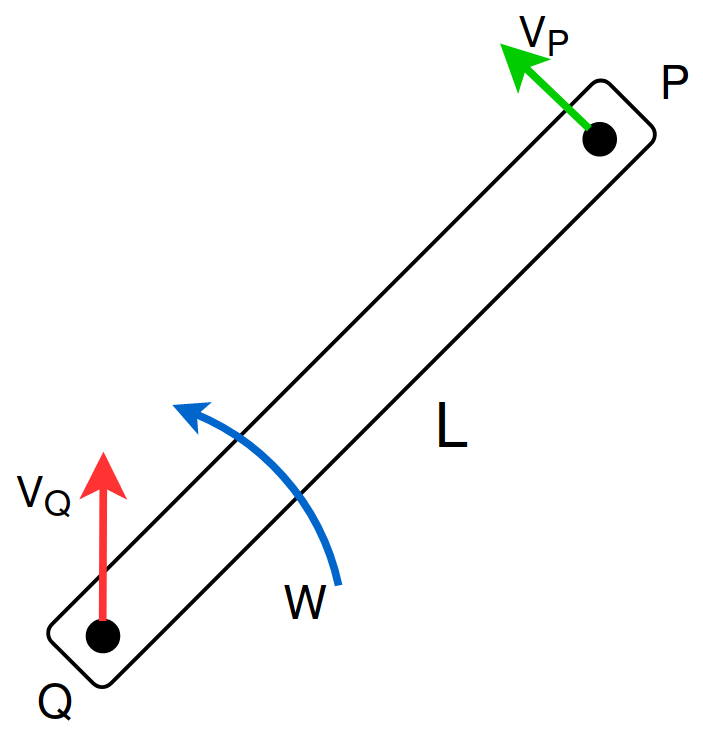
\includegraphics[width=0.3\linewidth]{images/movimiento_cuerpo_rigido.png}
    \caption{Movimiento de un cuerpo rígido}
    \label{fig:movimientocuerporigido}
\end{figure}

Se consideran $ V_{01}, V_{02}, V_{03}, V_{04} $ nulos dado que no existe deslizamiento entre las ruedas y el piso, además si todas las ruedas tienen el mismo radio, podemos expresar:

$$ V_{R1} = \omega_1 \times r $$
$$ V_{R2} = \omega_2 \times r $$
$$ V_{R3} = \omega_3 \times r $$
$$ V_{R4} = \omega_4 \times r $$

Ahora, podemos analizar el marco de referencia de la rueda respecto al marco de referencia del robot. Para ello:

\begin{figure}[H]
    \centering
    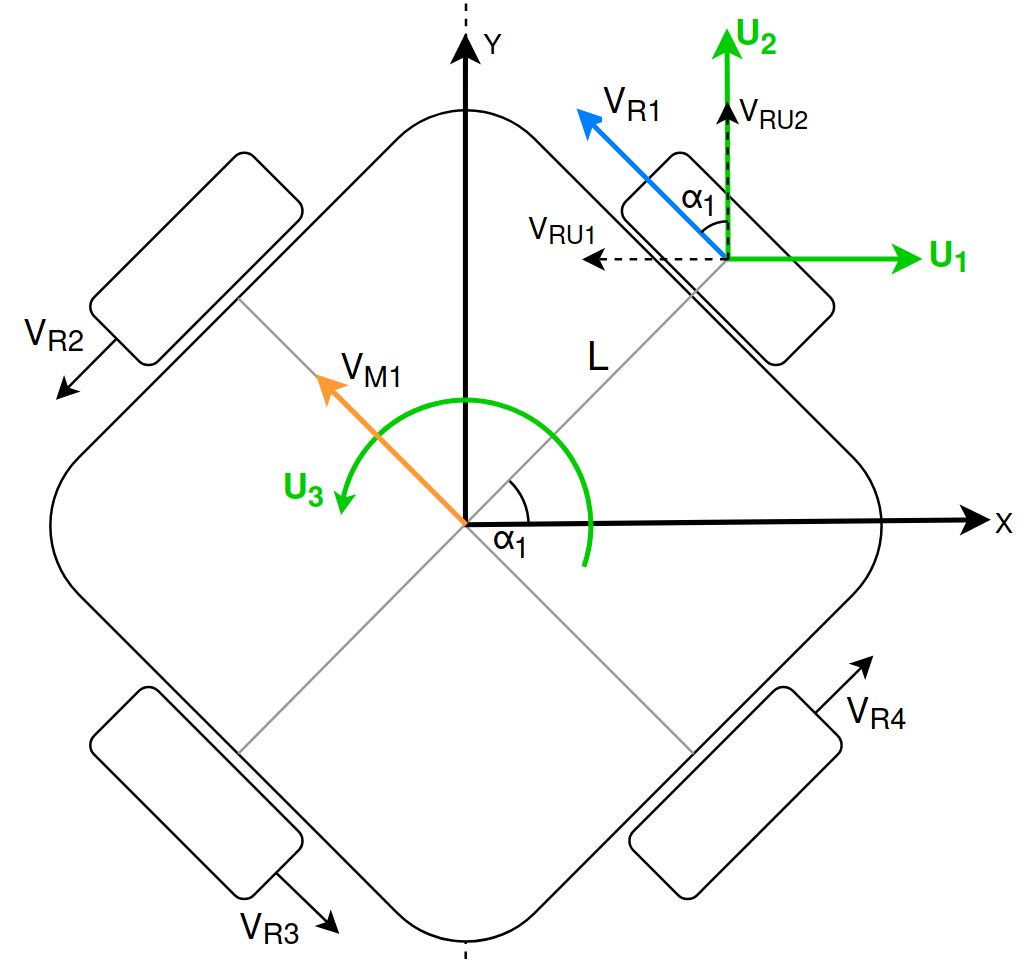
\includegraphics[width=0.6\linewidth]{images/modelo_cinematico_robot_vector.png}
    \caption{Vectores del robot en el marco de referencia local}
    \label{fig:robotmarcoreflocal}
\end{figure}

Se plantea el caso para una de las ruedas. Para obtener el vector $V_{R1}$ en base al marco de referencia denotado por $U_1$, $U_2$ y $U_3$, podemos hacer:

$$ V_{R1} = V_{M1} + U_3 \times L $$

De modo que podemos expresar $V_{M1}$ en función de $U_1$ y $U_2$:

$$ V_{M1} = V_{RU_1} + V_{RU_2} $$
$$ V_{M1} = -U_1 \cdot sen(\alpha_1) + U_2 \cdot cos(\alpha_1) $$

Obteniendo finalmente que:

$$ V_{R1} = -U_1 \cdot sen(\alpha_1) + U_2 \cdot cos(\alpha_1) + U_3 \times L $$

Al realizar el mismo procedimiento para las demás ruedas obtenemos:

$$ V_{R1} = -U_1 \cdot sen(\alpha_1) + U_2 \cdot cos(\alpha_1) + U_3 \times L $$
$$ V_{R2} = -U_1 \cdot sen(\alpha_1) + U_2 \cdot cos(\alpha_1) + U_3 \times L $$
$$ V_{R4} = -U_1 \cdot sen(\alpha_1) + U_2 \cdot cos(\alpha_1) + U_3 \times L $$
$$ V_{R3} = -U_1 \cdot sen(\alpha_1) + U_2 \cdot cos(\alpha_1) + U_3 \times L $$

Ahora bien, si $U_1$, $U_2$ y $U_3$ están alineados respecto al marco de referencia global $0XY$, podemos expresar:

$$ \begin{bmatrix} U_1 \\ U_2 \\ U_3 \end{bmatrix} = \begin{bmatrix} V_x \\ V_y \\ V_\theta \end{bmatrix} $$

Entonces ahora podemos hacer la siguiente igualdad con lo obtenido:

$$ \omega_1 \times r = -V_x \cdot sen(\alpha_1) + V_y \cdot cos(\alpha_1) + V_\theta \times L $$
$$ \omega_2 \times r = -V_x \cdot sen(\alpha_2) + V_y \cdot cos(\alpha_2) + V_\theta \times L $$
$$ \omega_3 \times r = -V_x \cdot sen(\alpha_3) + V_y \cdot cos(\alpha_3) + V_\theta \times L $$
$$ \omega_4 \times r = -V_x \cdot sen(\alpha_4) + V_y \cdot cos(\alpha_4) + V_\theta \times L $$

Originalmente partimos de que necesitamos una matriz de conversión de modo que podamos obtener las velocidades de las ruedas en base a un vector dado, donde la entrada es $V_x, V_y$ expresadas en $[m/seg]$ y $V_\theta$ expresada en $[RPM]$. Por otra parte, la salida $\omega_n$ se determina en $[rad/seg]$:

$$ \begin{bmatrix} w_1 \\ w_2 \\ w_3 \\ w_4 \\ \end{bmatrix} = IK \cdot \begin{bmatrix} V_x \\ V_y \\ V_\theta \\ \end{bmatrix} $$

Con las expresiones anteriores, obtenemos que la matriz cinemática inversa se puede expresar como:

$$ IK = 
    \frac{1}{r}
    \cdot
    \begin{bmatrix}
        {-sen(\alpha_1)} & {cos(\alpha_1)} & L \\
        {-sen(\alpha_2)} & {cos(\alpha_2)} & L \\
        {-sen(\alpha_3)} & {cos(\alpha_3)} & L \\
        {-sen(\alpha_4)} & {cos(\alpha_4)} & L \\
    \end{bmatrix} $$

De modo que podemos expresar la ecuación para obtener las velocidades de las ruedas expresadas en $[rad/seg]$ como se muestra debajo.

$$ \begin{bmatrix} w_1 \\ w_2 \\ w_3 \\ w_4 \\ \end{bmatrix} = \frac{1}{r} \cdot \begin{bmatrix}
    {-sen(\frac{\pi}{4})} & {cos( \frac{\pi}{4})} & L \\
    {-sen(\frac{3\pi}{4})} & {cos(\frac{3\pi}{4})} & L \\
    {-sen(\frac{5\pi}{4})} & {cos(\frac{5\pi}{4})} & L \\
    {-sen(\frac{7\pi}{4})} & {cos(\frac{7\pi}{4})} & L \\
\end{bmatrix} \cdot
\begin{bmatrix} V_x \\ V_y \\ V_\theta \\ \end{bmatrix} $$

Dado que las MotorTask de cada una de las ruedas recibe el setpoint en $[RPM]$, debemos hacer una conversión a esa unidad. Por lo que planteamos una matriz que convierta los valores de las dos primeras columnas de la matriz cinemática, que son los coeficientes que nos interesa convertir a $[RPM]$, dado que los de la última columna ya están expresados en esa unidad.

$$ \begin{bmatrix} w_1 \\ w_2 \\ w_3 \\ w_4 \\ \end{bmatrix} =
    \frac{1}{r}
    \cdot
    \begin{bmatrix}
        {-sen(\frac{\pi}{4})} & {cos( \frac{\pi}{4})} & L \\
        {-sen(\frac{3\pi}{4})} & {cos(\frac{3\pi}{4})} & L \\
        {-sen(\frac{5\pi}{4})} & {cos(\frac{5\pi}{4})} & L \\
        {-sen(\frac{7\pi}{4})} & {cos(\frac{7\pi}{4})} & L \\
    \end{bmatrix}
    \cdot
    \begin{bmatrix}
        {\frac{60}{2 \pi}} & {0} & {0} \\
        {0} & {\frac{60}{2 \pi}} & {0} \\
        {0} & {0} & {1}                \\
    \end{bmatrix}
    \cdot
    \begin{bmatrix} V_x \\ V_y \\ V_\theta \\ \end{bmatrix} $$


\textbf{Cinemática Directa} \mbox{} \vspace{8pt}

Para lograr el control del robot sobre el plano es necesario hacer una comparación entre el vector de movimiento deseado y un vector de movimiento inferido en base a la medición de la velocidad de las ruedas, de modo que se cierra el lazo de control. El error existente entre el vector real y el deseado es debido a que los motores no establecen las RPM inmediatamente por cuestiones de inercia e imperfecciones en el terreno.

Para obtener el vector de velocidad lineal real que efectivamente realiza el robot, hacemos uso de las mediciones de velocidad angular en cada rueda y se ingresan a la ecuación cinemática directa. Esta matriz se obtiene a partir de la pseudoinversa de la matriz cinemática inversa. \cite{islassistcontrolomni}

De modo que, en primer lugar obtenemos la matriz de conversión que nos permite obtener el vector lineal en base a las velocidades de las ruedas expresadas en $[rad/seg]$:

$$ \begin{bmatrix} V_x \\ V_y \\ V_\theta \\ \end{bmatrix} = DK \cdot \begin{bmatrix} w_1 \\ w_2 \\ w_3 \\ w_4 \\ \end{bmatrix} $$

Luego, al realizar la pseudoinversa de la matriz $IK$:

$$  DK = 
    r
    \cdot 
    \begin{bmatrix}
        {\frac{-sen(\alpha_1)}{2}} & {\frac{-sen(\alpha_2)}{2}} & {\frac{-sen(\alpha_3)}{2}} & {\frac{-sen(\alpha_4)}{2}} \\
        {\frac{cos(\alpha_1)}{2}}  & {\frac{cos(\alpha_2)}{2}}  & {\frac{cos(\alpha_3)}{2}}  & {\frac{cos(\alpha_4)}{2}}  \\
        {\frac{1}{4L}}  & {\frac{1}{4L}}  & {\frac{1}{4L}}  & {\frac{1}{4L}}  \\
    \end{bmatrix} $$

Por lo que obtenemos la siguiente expresión para obtener el vector de movimiento del robot dependiendo de las velocidades de las ruedas:

$$ \begin{bmatrix} V_x \\ V_y \\ V_\theta \\ \end{bmatrix} = 
    r
    \cdot 
    \begin{bmatrix}
        {\frac{-sen(\alpha_1)}{2}} & {\frac{-sen(\alpha_2)}{2}} & {\frac{-sen(\alpha_3)}{2}} & {\frac{-sen(\alpha_4)}{2}} \\
        {\frac{cos(\alpha_1)}{2}}  & {\frac{cos(\alpha_2)}{2}}  & {\frac{cos(\alpha_3)}{2}}  & {\frac{cos(\alpha_4)}{2}}  \\
        {\frac{1}{4L}}  & {\frac{1}{4L}}  & {\frac{1}{4L}}  & {\frac{1}{4L}}  \\
    \end{bmatrix}
    \cdot
    \begin{bmatrix} w_1 \\ w_2 \\ w_3 \\ w_4 \\ \end{bmatrix} $$

Esta expresión toma las velocidades angulares de las ruedas en $[rad/seg]$, por lo que necesitamos convertir la entrada para que pueda ser $[RPM]$. Para ello planteamos una matriz que solo convierta los valores de las dos primeras filas, que son los coeficientes que nos interesa convertir a $[RPM]$, dado que los de la última fila ya están expresados en esa unidad.

$$ \begin{bmatrix} V_x \\ V_y \\ V_\theta \\ \end{bmatrix} = 
    r
    \cdot 
    \begin{bmatrix}
        {\frac{2\pi}{60}} & {0} & {0}  \\
        {0} & {\frac{2\pi}{60}} & {0} \\
        {0} & {0} & {1} \\
    \end{bmatrix}
    \cdot
    \begin{bmatrix}
        {\frac{-sen(\alpha_1)}{2}} & {\frac{-sen(\alpha_2)}{2}} & {\frac{-sen(\alpha_3)}{2}} & {\frac{-sen(\alpha_4)}{2}} \\
        {\frac{cos(\alpha_1)}{2}}  & {\frac{cos(\alpha_2)}{2}}  & {\frac{cos(\alpha_3)}{2}}  & {\frac{cos(\alpha_4)}{2}}  \\
        {\frac{1}{4L}}  & {\frac{1}{4L}}  & {\frac{1}{4L}}  & {\frac{1}{4L}}  \\
    \end{bmatrix}
    \cdot
    \begin{bmatrix} w_1 \\ w_2 \\ w_3 \\ w_4 \\ \end{bmatrix} $$


\paragraph{Implementación} \mbox{} \vspace{8pt}

Para la implementación se propuso que el modelo cinemático sea contenido dentro de la MasterTask dado que es quien recibe el feedback de todas las tareas MotorTask y conoce el estado actual de cada uno de los motores. Un diagrama de secuencia se detalla más adelante en este capítulo.

\begin{figure}[H]
    \centering
    \hspace*{-0.75cm}
    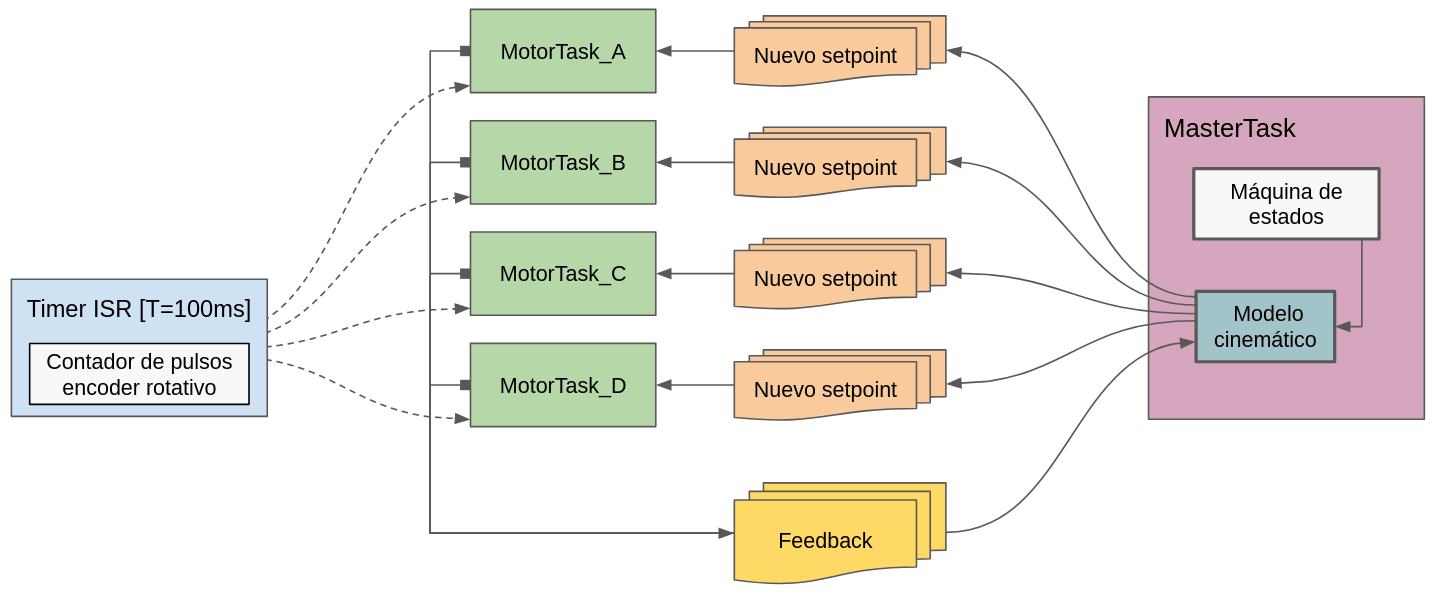
\includegraphics[width=1.1\linewidth]{images/diag_comp_esp32_modelo_cinem.png}
    \caption{Estructura de control de los motores con el Modelo Cinemático}
    \label{fig:diagcomponentesp32modelocinem}
\end{figure}


\subsubsection{Odometría}

La odometría es el proceso mediante el cual un robot estima su posición y orientación en el espacio a lo largo del tiempo. Esta técnica se utiliza para obtener una aproximación de la trayectoria recorrida por el robot, a partir de los desplazamientos medidos en sus ruedas o actuadores, generalmente utilizando sensores como pueden ser encoders rotativos o lineales.

Dado que necesitamos estimar la posición y orientación del robot en el espacio a lo largo del tiempo, nos podemos basar en las lecturas de los sensores de las ruedas. Para inferir la distancia recorrida podemos medir las velocidades angulares o la distancia recorrida de cada una de las cuatro ruedas en simultáneo. Estos datos se obtienen a partir de los encoders rotativos instalados en las ruedas.

Se probaron distintas alternativas para el proceso de odometría. Primeramente se probó de modo que cada rueda recibe la distancia que debe recorrer el robot y de modo independiente mide cuanto recorre para determinar si debe detenerse o no. Concluimos que esta técnica tiene algunos problemas porque no considera a nivel global el movimiento del robot y como influyen las perturbaciones de las demás ruedas sobre una de ellas. Es por ello que optamos por hacer uso del modelo cinemático para realizar la odometría. Este método no excluye de errores al proceso, pero tiene en consideración todas las ruedas al momento de determinar la distancia recorrida por el robot dada la sumatoria de la acción de todas ellas. \cite{palacinodometry}

La odometría se basa en el uso del modelo cinemático para convertir estas velocidades angulares en velocidades lineales y angulares del robot en el plano, es decir, obtener un vector de movimiento en base a las mediciones. Para ello, el primer paso en el proceso es utilizar las ecuaciones del modelo cinemático directo para calcular las velocidades lineales y angulares en el instante $t$ a partir de las velocidades de las ruedas: ($V_xt$, $V_yt$, $V_\theta t$). Posteriormente se pueden integrar estas velocidades a lo largo del tiempo para estimar la posición ($x, y$) y la orientación ($\theta$) del robot. La integración se realiza mediante métodos numéricos, típicamente utilizando un enfoque de integración discreta, como el método de Euler. Por lo que en cada instante de tiempo que se toma una medición, se actualiza la posición y orientación del robot utilizando las siguientes ecuaciones, donde ($\Delta$t) es el intervalo de tiempo entre dos mediciones consecutivas:

$$ x_{t+1} = x_t + V_xt \cdot \Delta t $$

$$ y_{t+1} = y_t + V_yt \cdot \Delta t $$

$$ \theta_{t+1} = \theta_t + V_\theta t \cdot \Delta t $$

Es importante considerar que la odometría realizada para ruedas puede acumular errores debido a factores como el deslizamiento de las ruedas, inexactitudes en las mediciones de los encoders o imprecisiones en los cálculos. Por lo tanto, es común combinar la odometría con otros métodos de localización, como el uso de sensores adicionales (LIDAR, cámaras, etc.) y técnicas de fusión de datos (como los filtros de Kalman), para mejorar la precisión y robustez de la estimación de la posición del robot.

Para la realización de las pruebas colocamos marcas en el piso a 1 metro de distancia entre sí y realizamos iteraciones para verificar que la odometría opera dentro de los rangos de precisión establecidos.


\subsubsection{Envío y recepción de comandos}

Se implementó un sistema de comunicación basado en el protocolo MQTT (Message Queuing Telemetry Transport) para enviar y recibir informacion del robot. Se envían vectores a recorrer con una estructura de datos a modo de tupla de valores que representa la distancia a recorrer, las velocidades lineales y angulares del robot: $distancia [m]$, $V_x [m/seg]$, $V_y [m/seg]$ y $V_\theta [RPM]$.

Además, el robot es capaz de enviar información por medio de MQTT sobre la odometría y el estado en tiempo real. Esto resulta útil dado que posibilita monitorear el estado del robot y realizar ajustes si es necesario.

Por un lado, las velocidades $V_x$ y $V_y$ determinan un sentido de movimiento en linea recta sobre el plano. Por otro lado, $V_\theta$ controla la rotación del robot sobre su propio eje, permitiéndole girar en el plano horizontal.

Cuando se envía una tupla de valores de velocidad mediante MQTT, el robot calcula la velocidad para cada rueda usando el modelo cinemático y establece los motores a la velocidad estipulada, luego se detiene cumplida la distancia recorrida. En la Figura \ref{fig:diagcomponentesp32conmodelocinem} se muestra un diagrama de secuencia con los componentes integrados hasta el momento.

\begin{figure}[htb]
    \centering
    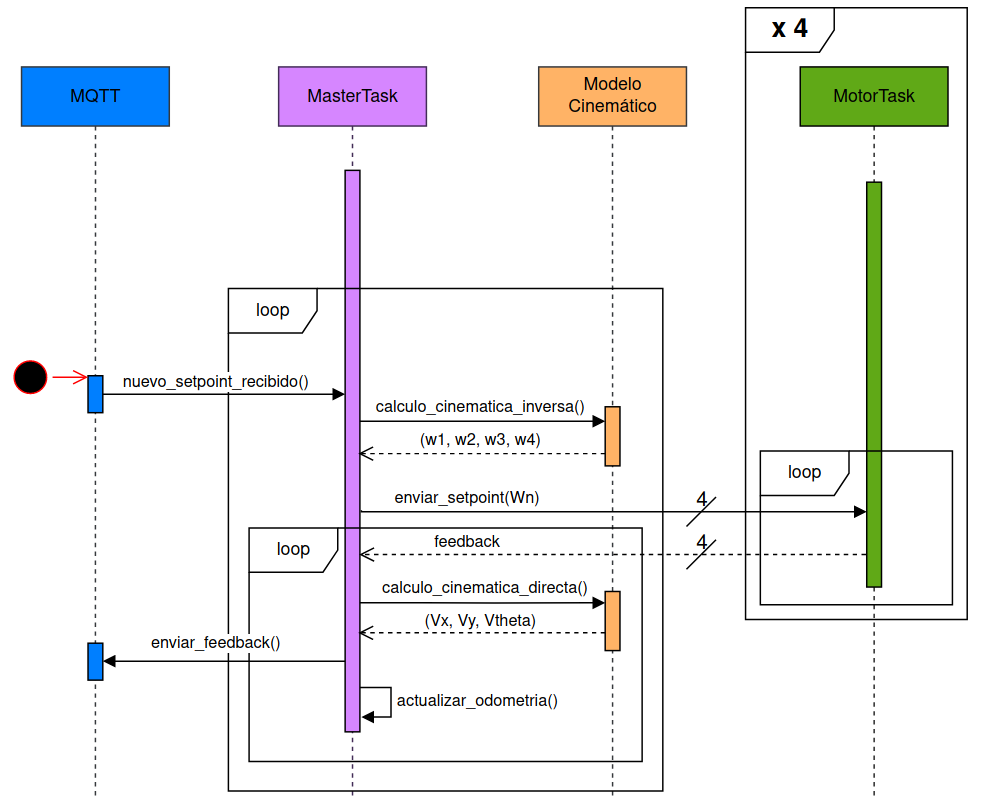
\includegraphics[width=1\linewidth]{images/diag_secuencia_full_modelo_cinematico.png}
    \caption{Diagrama de secuencia de la ESP32 con el Modelo Cinemático}
    \label{fig:diagcomponentesp32conmodelocinem}
\end{figure}


\subsubsection{Campo de pruebas}

En cualquier estudio experimental, es vital controlar todas las variables posibles para aislar el efecto de las variables independientes. La superficie sobre la que se desplaza el robot puede influir significativamente en su comportamiento, ya que las irregularidades de la misma pueden inducir deslizamientos o atascos.

La elección de una superficie determinada, consistente y constante en cada experimento es crucial para asegurar la fiabilidad de los resultados obtenidos, al proporcionar un entorno controlado. Mantener una superficie constante permite replicar las condiciones experimentales y comparar resultados de manera precisa y predecible. Si la superficie varía, se introducen variables adicionales que pueden afectar el desempeño del robot, dificultando la comparación entre experimentos.

En primera instancia, la superficie sobre la cual comenzamos las pruebas del prototipo fue el suelo del Laboratorio. En los sucesivos experimentos notamos cierta inconsistencia entre cada iteración, manteniendo los parámetros de funcionamiento constantes. En búsqueda de mejorar la consistencia entre los experimentos, hicimos algunas pruebas sobre un tablón de madera lisa y notamos que la mejoría es sustancial. En consecuencia, se dispone de una superficie de madera sobre la cual realizamos las subsiguientes pruebas.


\subsection{Testing y pruebas}

% https://en.wikibooks.org/wiki/LaTeX/Tables

\begin{testtableformat}
    \hline \rowcolor{test_header_color}
        Test ID             & TC\_01\_00 \\
    \hline
        Tipo de test        & Test unitario \\
    \hline
        Objeto de prueba    & Comunicación inalámbrica \\
    \hline
        Requerimiento       & RF6 \\
    \hline
        Nombre              & Comunicación inalámbrica para monitoreo y envío de comandos por MQTT \\
    \hline
        Descripción         & Verificar que los comandos son recibidos correctamente en el robot y que el robot envía información de estado en el formato correcto \\
    \hline
        Precondición        & PRECOND\_A \\
    \hline
        Pasos del test      & \begin{enumerate}
                                \item Enviar un nuevo setpoint con parámetros de distancia [50cm $\sim$ 200cm] y velocidad $\pm$[0.25m/seg $\sim$ 0.75m/seg]
                                \item Verificar que el robot recibe el comando correctamente y que envía reportes
                                \item Repetir desde el paso 1) con diferentes valores
                            \end{enumerate} \\
    \hline
        Resultado esperado  & El robot recibe e interpreta los comandos, al mismo tiempo que reporta información sobre su estado periódicamente \\
    \hline
        Resultado obtenido  & El robot realiza el comportamiento esperado, envía, recibe e interpreta comandos \\
    \hline
        Observaciones       & - \\
    \hline
\end{testtableformat}


\begin{testtableformat}
    \hline \rowcolor{test_header_color}
        Test ID             & TC\_01\_01 \\
    \hline
        Tipo de test        & Test unitario \\
    \hline
        Objeto de prueba    & PWM - Medidor de RPM \\
    \hline
        Requerimiento       & RF1 - RF5 \\
    \hline
        Nombre              & Medidor de RPM \\
    \hline
        Descripción         & Comprobar que al establecer el motor a determinada velocidad ésta se corresponda con la medición obtenida por el medidor de RPM \\
    \hline
        Precondición        & PRECOND\_A \\
    \hline
        Pasos del test      & \begin{enumerate}
                                \item Enviar un valor de PWM al controlador del motor entre [0 $\sim$ 1023]
                                \item Verificar que el motor se establece a la velocidad deseada y que el medidor de RPM informa el valor correcto
                                \item Repetir desde el paso 1) con diferentes valores
                            \end{enumerate} \\
    \hline
        Resultado esperado  & Se obtiene el valor correcto de RPM medido en cada iteración \\
    \hline
        Resultado obtenido  & En todas las iteraciones las mediciones reportan una velocidad cercana a la establecida \\
    \hline
        Observaciones       & La velocidad máxima que podemos obtener del motor sin carga son 92 RPM (PWM = 1023) y el motor comienza a girar continuamente cuando las RPM se establecen en una velocidad mínima de 55 RPM (PWM $\cong$ 420) \\
    \hline
\end{testtableformat}


\begin{testtableformat}
    \hline \rowcolor{test_header_color}
        Test ID             & TC\_01\_02 \\
    \hline
        Tipo de test        & Test de integración \\
    \hline
        Objeto de prueba    & PID - PWM - Medidor de RPM \\
    \hline
        Requerimiento       & RF1 - RF5 \\
    \hline
        Nombre              & PID sin carga \\
    \hline
        Descripción         & Verificar que el PID establece correctamente la velocidad de la rueda al recibir el setpoint en RPM sin carga vinculada a la rueda \\
    \hline
        Precondición        & PRECOND\_A \\
    \hline
        Pasos del test      & \begin{enumerate}
                                \item Enviar un valor de RPM al controlador PID del motor entre [0 $\sim$ 92] RPM
                                \item Verificar que el motor se establece a las RPM deseadas y que el medidor de RPM informa el valor correcto
                                \item Repetir desde el paso 1) con diferentes valores
                            \end{enumerate} \\
    \hline
        Resultado esperado  & Se obtiene el valor de RPM correcta en cada iteración \\
    \hline
        Resultado obtenido  & En todas las iteraciones se obtuvo que la rueda gira a una velocidad cercana a la establecida \\
    \hline
        Observaciones       & La velocidad máxima que podemos obtener del motor sin carga son 92 RPM y el motor comienza a girar continuamente cuando las RPM se establecen en una velocidad mínima de 55 RPM \\
    \hline
\end{testtableformat}


\begin{testtableformat}
    \hline \rowcolor{test_header_color}
        Test ID             & TC\_01\_03 \\
    \hline
        Tipo de test        & Test de integración \\
    \hline
        Objeto de prueba    & PID - PWM - Medidor de RPM \\
    \hline
        Requerimiento       & RF1 - RF5 \\
    \hline
        Nombre              & PID con carga \\
    \hline
        Descripción         & Verificar que el PID establece correctamente la velocidad de la rueda al recibir el setpoint en RPM con una carga aproximadamente igual al peso del robot \\
    \hline
        Precondición        & PRECOND\_A \\
    \hline
        Pasos del test      & \begin{enumerate}
                                \item Enviar un valor de RPM al controlador PID del motor entre [0 $\sim$ 92] RPM
                                \item Verificar que el motor se establece a las RPM deseadas y que el medidor de RPM informa el valor correcto
                                \item Repetir desde el paso 1) con diferentes valores
                            \end{enumerate} \\
    \hline
        Resultado esperado  & Se obtiene el valor de RPM correcta en cada iteración \\
    \hline
        Resultado obtenido  & En todas las iteraciones se obtuvo que la rueda gira a una velocidad cercana a la establecida \\
    \hline
        Observaciones       & La velocidad máxima que podemos obtener del motor con una carga presente son 88 RPM y el motor comienza a girar continuamente cuando las RPM se establecen en una velocidad mínima de 63 RPM \\
    \hline
\end{testtableformat}


\begin{testtableformat}
    \hline \rowcolor{test_header_color}
        Test ID             & TC\_01\_04 \\
    \hline
        Tipo de test        & Test unitario \\
    \hline
        Objeto de prueba    & Modelo Cinemático \\
    \hline
        Requerimiento       & RF2 - RF4 \\
    \hline
        Nombre              & Modelo Cinemático en línea recta \\
    \hline
        Descripción         & Comprobar que el Modelo Cinemático calcula adecuadamente las velocidades de las ruedas según un setpoint en línea recta \\
    \hline
        Precondición        & PRECOND\_B \\
    \hline
        Pasos del test      & \begin{enumerate}
                                \item Enviar al Modelo Cinemático un vector de velocidad en linea recta con valores entre $\pm$[0.25m/seg $\sim$ 0.75m/seg]
                                \item Colocar cada una de las ruedas a la velocidad calculada por el Modelo Cinemático y verificar que el robot se mueve a lo largo del vector definido
                                \item Repetir desde el paso 1) con diferentes valores
                            \end{enumerate} \\
    \hline
        Resultado esperado  & El robot se mueve en línea recta en la dirección del vector dado por $V_x$ y $V_y$ \\
    \hline
        Resultado obtenido  & Se observa que el robot realiza el comportamiento esperado \\
    \hline
        Observaciones       & - \\
    \hline
\end{testtableformat}


\begin{testtableformat}
    \hline \rowcolor{test_header_color}
        Test ID             & TC\_01\_05 \\
    \hline
        Tipo de test        & Test unitario \\
    \hline
        Objeto de prueba    & Modelo Cinemático \\
    \hline
        Requerimiento       & RF2 - RF4 \\
    \hline
        Nombre              & Modelo Cinemático en trayectorias curvas \\
    \hline
        Descripción         & Comprobar que el Modelo Cinemático calcula adecuadamente las velocidades de las ruedas según un setpoint con velocidad rotacional distinta de cero \\
    \hline
        Precondición        & PRECOND\_B \\
    \hline
        Pasos del test      & \begin{enumerate}
                                \item Enviar al Modelo Cinemático un vector de velocidad lineal nula y velocidad rotacional distinta de cero con valores entre $\pm$[0RPM $\sim$ 30RPM]
                                \item Colocar cada una de las ruedas a la velocidad calculada por el Modelo Cinemático y verificar que el robot gira sobre su eje según la velocidad rotacional dada
                                \item Repetir desde el paso 1) con diferentes valores
                            \end{enumerate} \\
    \hline
        Resultado esperado  & El robot gira sobre su eje a distintas velocidades \\
    \hline
        Resultado obtenido  & Se observa que el robot realiza el comportamiento esperado \\
    \hline
        Observaciones       & - \\
    \hline
\end{testtableformat}


\begin{testtableformat}
    \hline \rowcolor{test_header_color}
        Test ID             & TC\_01\_06 \\
    \hline
        Tipo de test        & Test unitario \\
    \hline
        Objeto de prueba    & Modelo Cinemático \\
    \hline
        Requerimiento       & RF2 - RF4 \\
    \hline
        Nombre              & Modelo Cinemático en trayectorias elípticas (lineal y curva en simultáneo) \\
    \hline
        Descripción         & Comprobar que el Modelo Cinemático calcula adecuadamente las velocidades de las ruedas según un vector de movimiento dado por velocidades lineales y velocidades angulares al mismo tiempo \\
    \hline
        Precondición        & PRECOND\_B \\
    \hline
        Pasos del test      & \begin{enumerate}
                                \item Enviar al Modelo Cinemático un vector de velocidad lineal y rotacional distintas de cero con valores para $V_x$ y $V_y$ entre $\pm$[0.25m/seg $\sim$ 0.75m/seg] y $V_r$ entre $\pm$[0RPM $\sim$ 30RPM]
                                \item Colocar cada una de las ruedas a la velocidad calculada por el Modelo Cinemático y verificar que el robot describe una trayectoria elíptica que se corresponde con el vector dado
                                \item Repetir desde el paso 1) con diferentes valores
                            \end{enumerate} \\
    \hline
        Resultado esperado  & El robot realiza trayectorias elípticas a distintas velocidades y radios de movimiento \\
    \hline
        Resultado obtenido  & El robot describe una trayectoria elíptica variable en radio y velocidad según se modifique el setpoint \\
    \hline
        Observaciones       & Al inicio hasta su convergencia, se observa un patrón en espiral y luego se torna un recorrido constante \\
    \hline
\end{testtableformat}


\begin{testtableformat}
    \hline \rowcolor{test_header_color}
        Test ID             & TC\_01\_07 \\
    \hline
        Tipo de test        & Test de integración \\
    \hline
        Objeto de prueba    & Odometría - Modelo cinemático \\
    \hline
        Requerimiento       & RF2 - RF3 - RF4 - RF5 \\
    \hline
        Nombre              & Odometría en línea recta \\
    \hline
        Descripción         & Verificar que el robot recorre la distancia establecida \\
    \hline
        Precondición        & PRECOND\_B \\
    \hline
        Pasos del test      & \begin{enumerate}
                                \item Enviar al robot un setpoint en linea recta de distancia entre [50cm $\sim$ 400cm] y velocidad $\pm$[0.25m/seg $\sim$ 0.75m/seg]
                                \item Verificar que el robot recorre el vector dado a lo largo de la distancia determinada
                                \item Repetir desde el paso 1) con diferentes valores
                            \end{enumerate} \\
    \hline
        Resultado esperado  & El robot recorre la distancia establecida \\
    \hline
        Resultado obtenido  & El robot a distancias menores a 20cm no logra una buena precisión. Con distancias de al menos 35cm se obtiene una buena precisión en la medición, de alrededor de +-3cm. \\
    \hline
        Observaciones       & Se probó hasta recorridos de 4 metros por limitaciones de espacio.  \\
    \hline
\end{testtableformat}


\begin{testtableformat}
    \hline \rowcolor{test_header_color}
        Test ID             & TC\_01\_08 \\
    \hline
        Tipo de test        & Test de integración \\
    \hline
        Objeto de prueba    & Odometría - Modelo cinemático \\
    \hline
        Requerimiento       & RF2 - RF3 - RF4 - RF5 \\
    \hline
        Nombre              & Odometría en trayectorias curvas \\
    \hline
        Descripción         & Verificar que el robot recorre la distancia establecida \\
    \hline
        Precondición        & PRECOND\_B \\
    \hline
        Pasos del test      & \begin{enumerate}
                                \item Enviar al robot un setpoint de trayectoria curva con distancia entre [50cm $\sim$ 400cm], velocidad lineal entre $\pm$[0.25m/seg $\sim$ 0.75m/seg] y velocidad rotacional entre $\pm$[0RPM $\sim$ 30RPM]
                                \item Verificar que el robot recorre el vector dado a lo largo de la distancia determinada
                                \item Repetir desde el paso 1) con diferentes valores
                            \end{enumerate} \\
    \hline
        Resultado esperado  & El robot recorre la distancia establecida \\
    \hline
        Resultado obtenido  & El robot a distancias menores a 32cm no logra una buena precisión. Con distancias de al menos 40cm se obtiene una buena precisión en la medición, de alrededor de +-6cm. \\
    \hline
        Observaciones       & Se probó hasta recorridos de 4 metros por limitaciones de espacio.  \\
    \hline
\end{testtableformat}


\begin{testtableformat}
    \hline \rowcolor{test_header_color}
        Test ID             & TC\_01\_09 \\
    \hline
        Tipo de test        & Test de sistema \\
    \hline
        Objeto de prueba    & Comunicación inalámbrica - PID - Modelo cinemático - Odometría \\
    \hline
        Requerimiento       & RF1 - RF2 - RF3 - RF4 - RF5 - RF6 \\
    \hline
        Nombre              & Prueba de sistema integrado \\
    \hline
        Descripción         & Comprobar que el robot realiza trayectorias en una dirección y longitud determinadas, además de reportar información de estado \\
    \hline
        Precondición        & PRECOND\_B \\
    \hline
        Pasos del test      & \begin{enumerate}
                                \item Enviar al robot un setpoint con distancia entre [50cm $\sim$ 400cm] y velocidad lineal entre $\pm$[0.25m/seg $\sim$ 0.75m/seg]
                                \item Verificar que el robot recorre el vector dado a lo largo de la distancia determinada y que reporta periódicamente mediciones y estado actual
                                \item Repetir desde el paso 1) con diferentes valores
                            \end{enumerate} \\
    \hline
        Resultado esperado  & El robot responde correctamente al vector y la distancia establecida, además reporta periódicamente el estado de mediciones de distancia y velocidad \\
    \hline
        Resultado obtenido  & El robot recibe comandos de trayectorias con vectores y distancias determinadas, se observa que realiza las trayectorias de manera acorde dentro de los límites observados en las pruebas unitarias y de integración. Al mismo tiempo se reciben los reportes de estado periódicos por parte del robot \\
    \hline
        Observaciones       & Se probó hasta recorridos de 4 metros por limitaciones de espacio. \\
    \hline
\end{testtableformat}

\subsection{Resultados}

En esta iteración se logró efectivamente el desarrollo de un prototipo funcional del robot. Es capaz de recibir comandos, realizar trayectorias rectas y curvas, teniendo también mediciones de odometría.

Las cuatro ruedas son compensadas mediante un controlador PID cada una y se dispone del modelo cinemático para determinar el vector de movimiento.

\begin{figure}[H]
    \centering
    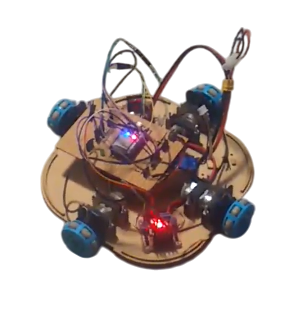
\includegraphics[trim={0 1cm 0 1cm}, clip, width=0.55\linewidth]{images/robot_sin_imanes_prototipo.png}
    \caption{Prototipo del robot}
    \label{fig:primerprototiporobot}
\end{figure}

\subsection{Riesgos superados}

En esta iteración se logro avanzar sobre el riesgo RI-03, pero para poder superarlo debemos explotar aun mas las capacidades del robot en las siguientes iteraciones.

Por otro lado, el riesgo RI-05 se logra superar en parte porque en esta iteración se incorporaron la mayoría de componentes esenciales.

\begin{center} \begin{tabular}{|p{0.10\linewidth}|p{0.65\linewidth}|}
\hline \rowcolor{test_header_color}
    ID & Descripción \\ 
\hline
    RI-03 & Prestaciones insuficientes de componentes. \\
\hline
    RI-05 & Dificultad en conseguir determinados componentes. \\
\hline
\end{tabular} \end{center}

\subsection{Conclusiones}

En primer lugar, se logró el control individual de velocidad y sentido de cada una de las ruedas y por otro lado, se desarrolló un modelo matemático del robot teniendo en cuenta el efecto de todas las ruedas.
En la presente iteración se obtuvo un prototipo que realiza mediciones de velocidad y distancia y las puede reportar inalámbricamente. Con todo esto podemos concluir que se alcanzó la meta de lograr un prototipo funcional superando varios desafíos para la cinemática y mecánica del robot.

\newpage
\section{Iteración 2: Prototipo mejorado}

\subsection{Introducción}
En el marco de la iteración anterior, se desarrolló un prototipo funcional que permitió validar la viabilidad técnica del sistema propuesto y sentar las bases para su evolución. Este trabajo destacó por identificar áreas clave de mejora que podrían optimizar su desempeño. Con base en estos hallazgos, la presente iteración se enfoca en mejorar el prototipo inicial, explorando la implementación de compensaciones en el sistema de control. Este enfoque tiene como objetivo principal incrementar la precisión, robustez y eficiencia del sistema, marcando un hito significativo en su desarrollo.

\subsection{Requerimientos}
En esta iteración abordaremos los siguientes requerimientos funcionales:

\begin{center} \begin{tabular}{|c|c|}
\hline
    ID & Descripción \\
\hline
    RF4 & El robot debe poder realizar trayectorias en línea recta y curvas. \\ 
\hline
    RF5 & El robot debe poder corregir su trayectoria mediante el uso de sensores. \\ 
\hline
\end{tabular} \end{center}

Por otra parte, los requerimientos no funcionales que trataremos son:

\begin{center} \begin{tabular}{|p{0.10\linewidth}|p{0.65\linewidth}|}
\hline
    ID & Descripción \\
\hline
    RNF1 & Debería tener tiempos de respuesta aceptables para el buen funcionamiento del sistema de control. \\
\hline
    RNF2 & El software debería contar con pruebas unitarias y de integración. \\
\hline
    RNF4 & El código debería contar con documentación.\\
\hline
\end{tabular} \end{center}

\subsection{Desarrollo}

\subsubsection{Compensación del modelo cinemático}

Dado el potencial del modelo cinemático, procedimos a compensar el sistema mediante la información provista por éste.

\paragraph{Compensación de movimiento lineal} \mbox{} \vspace{8pt}

En un caso real, existen variaciones que pueden provocar desviaciones en la ruta planeada debido a la textura o inclinación del suelo, imprecisiones o ruido en los sensores y el desgaste de las ruedas, así como otros factores mecánicos que pueden alterar la respuesta del robot a las órdenes de control.

Para abordar estos desafíos, se implementa un procedimiento de control que ajusta continuamente las velocidades de las ruedas en función de la retroalimentación recibida de los sensores y del modelo cinemático del robot. Se utilizan sensores para medir la posición y orientación actual del robot en el plano, inferida a partir de la odometría y las velocidades de las ruedas, para comparar estos datos con la trayectoria deseada y estimar los errores de posición y orientación. El modelo cinemático nos ayuda a  comprender cómo las velocidades de las ruedas individuales afectan el movimiento general del robot a través de ecuaciones matriciales que describen el comportamiento cinemático del robot.

Basado en los errores estimados y el modelo cinemático, se calculan las correcciones necesarias para las velocidades de las ruedas y se envían a los actuadores de las ruedas, logrando que el robot ajuste su movimiento de manera inmediata. \cite{rijalusalamkinematics} El proceso de medición, estimación, cálculo y aplicación de correcciones se repite continuamente a una frecuencia de $500[ms]$, equivalentes a 5 períodos de medición de RPM de cada rueda. En la Figura \ref{fig:diagramamodelocinemcompensado} podemos ver como se relacionan las variables.

\begin{figure}[htb]
    \centering
    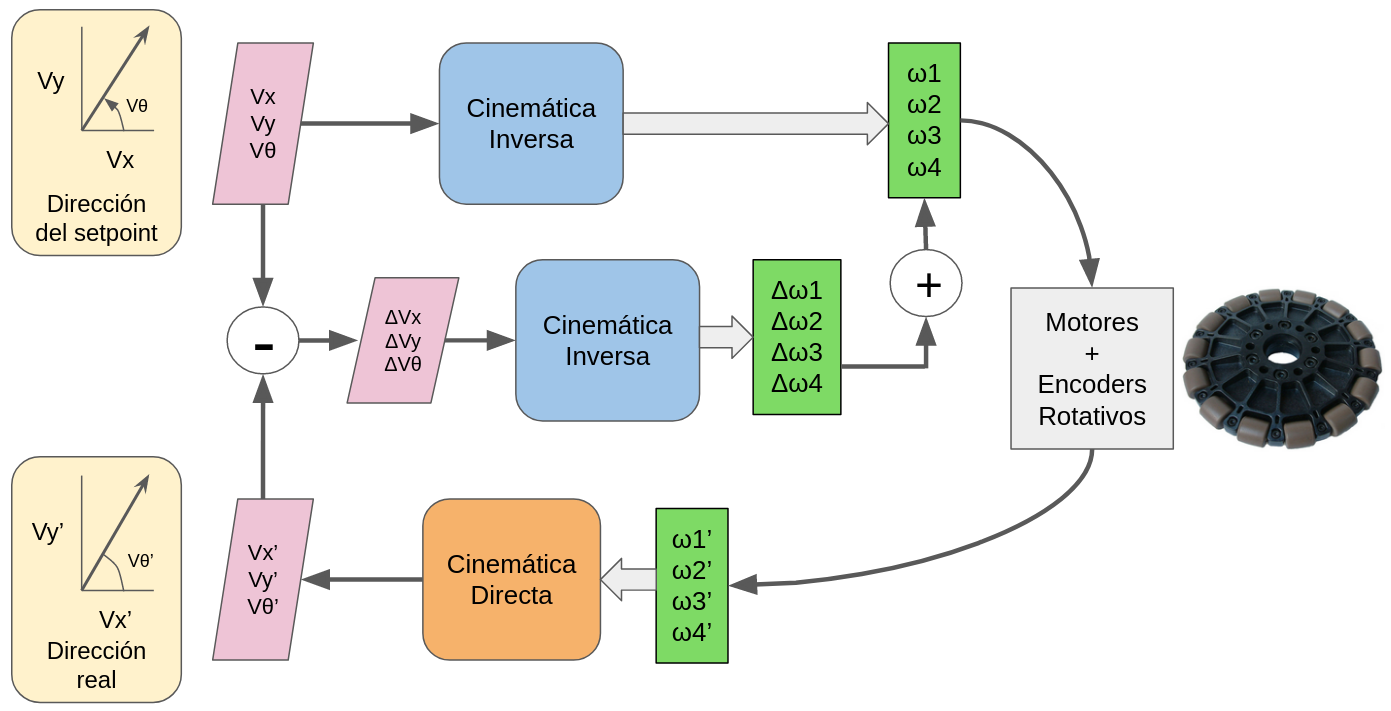
\includegraphics[width=1\linewidth]{images/diag_compensacion_modelo_cinem.png}
    \caption{Diagrama del Modelo Cinemático compensado}
    \label{fig:diagramamodelocinemcompensado}
\end{figure}

Los experimentos se realizaron en un entorno consistente con la iteración anterior y los resultados muestran una reducción significativa en los errores de trayectoria, demostrando la robustez del enfoque propuesto, de modo que el robot puede seguir trayectorias con desviaciones mínimas.

\paragraph{Compensación de movimiento rotacional} \mbox{} \vspace{8pt}

El enfoque propuesto es el de tener un acumulador basado en la odometría de $\theta$ que mide la distancia recorrida angularmente. El principio de funcionamiento es tal que aplica ajustes en la velocidad rotacional para compensar el desplazamiento, de modo que el robot intente llevar la distancia rotacional a cero nuevamente. Por ejemplo, si el robot detecta un desplazamiento hacia la derecha, se aumenta la velocidad rotacional hacia la izquierda para compensar el desfase en la cantidad determinada por la distancia rotacional. De este modo es posible corregir la orientación de movimiento. \\

En la Figura \ref{fig:diagsecuenciamodcinemcompens} se muestra un diagrama de secuencia sobre la implementación de la compensación del Modelo Cinemático.

\begin{figure}[htb]
    \centering
    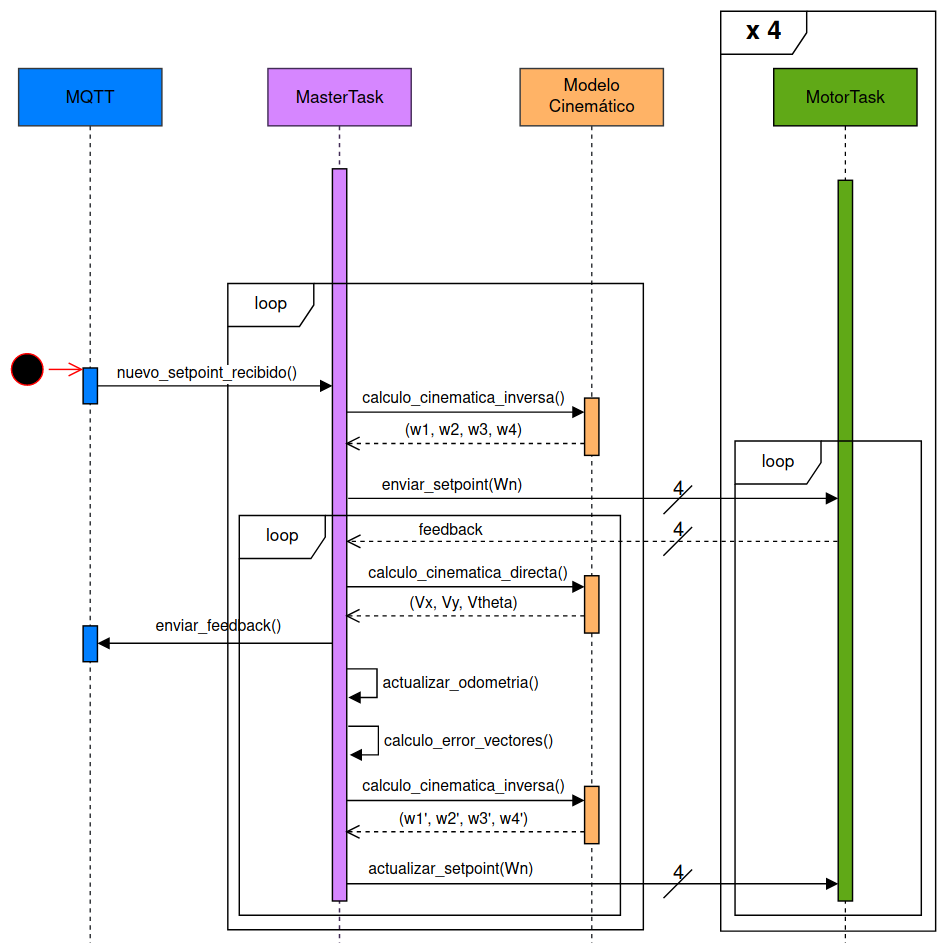
\includegraphics[width=1\linewidth]{images/diag_secuencia_modelo_cinematico_compensado.png}
    \caption{Diagrama de secuencia del Modelo Cinemático compensado}
    \label{fig:diagsecuenciamodcinemcompens}
\end{figure}




\subsubsection{Seguidor de línea}

A pesar de ser una herramienta fundamental para estimar la posición y orientación del robot, la odometría está sujeta a errores. Por lo que se hace necesario contar con un mecanismo adicional para poder detectar desviaciones en la trayectoria. Para esto se propone un seguidor de línea colocado de modo que el robot pueda detectar cuando se sale por fuera de las trayectorias determinadas por las líneas.

Un seguidor de línea es un sistema basado en sensores que detectan marcas en el entorno y utilizan esta información para ajustar la trayectoria del robot de manera automática.

La implementación de un seguidor de línea en robots omnidireccionales ofrece varias ventajas. En primer lugar, permite corregir desviaciones causadas por errores acumulativos en la odometría, ya que los sensores del seguidor de línea proporcionan información directa sobre la posición del robot respecto a la línea de referencia y en tiempo real.


\paragraph{Elección de método de seguimiento} \mbox{} \vspace{6pt}

Existen distintas técnicas para detectar una linea que un robot puede seguir. \\

\textbf{Seguidor de Línea Ultrasónico} \mbox{} \vspace{6pt} \\
Utiliza sensores ultrasónicos para detectar la presencia de una línea guía de la cual el robot debe mantenerse equidistante. Estos sensores emiten ondas sonoras de alta frecuencia y miden el tiempo que estas tardan en reflejarse al encontrar una superficie, lo que permite al robot seguir una trayectoria de manera precisa.

Entre sus ventajas, destaca su robustez, ya que no se ven afectados por factores como la suciedad o la iluminación, y su precisión, al detectar con alta exactitud la distancia hacia la línea guía. Sin embargo, estos sistemas presentan algunas desventajas, como la mayor complejidad y costo asociados con los sensores ultrasónicos, así como un alcance limitado en comparación con otros tipos de sensores. \cite{venkateshrfidultrasonic} \cite{aungultrasonic} \\


\textbf{Seguidor de Línea por Cámara} \mbox{} \vspace{6pt} \\
El seguidor de línea por cámara utiliza cámaras y algoritmos de procesamiento de imágenes para identificar y seguir líneas en el suelo de manera eficiente. Estas tecnologías permiten que el sistema sea altamente versátil, adaptándose a distintos tipos de líneas y patrones, al tiempo que proporcionan información adicional sobre el entorno que rodea al robot.

No obstante, esta solución presenta ciertos desafíos. Por un lado, requiere algoritmos avanzados de procesamiento de imágenes, lo que puede complicar su implementación. Por otro, su desempeño puede verse afectado por cambios en las condiciones de iluminación, lo que limita su eficacia en entornos variables. \cite{inianlinefollowcamera} \\


\textbf{Seguidor de Línea Ópticos} \mbox{} \vspace{6pt} \\
Los seguidores de línea ópticos son una de las implementaciones más comunes, ya que emplean sensores ópticos para detectar el contraste entre una línea dibujada en el suelo, generalmente negra, y el fondo, que suele ser blanco. Sensores como los fotodiodos o fototransistores envían señales al controlador del robot, permitiéndole ajustar su trayectoria para mantenerse sobre la línea. Entre las opciones disponibles, las versiones láser o infrarrojas son las más utilizadas.

Este sistema tiene como principales ventajas su simplicidad y bajo costo, ya que es relativamente sencillo de implementar, así como la amplia disponibilidad de estos dispositivos en el mercado. Sin embargo, también presenta algunas desventajas. Su rendimiento puede verse afectado por factores ambientales como la iluminación variable, el polvo, la suciedad y las superficies reflectantes, además de mostrar menor precisión en superficies no uniformes. Adicionalmente, las líneas pintadas en el suelo pueden desgastarse con el tiempo, requiriendo mantenimiento constante. \\


\textbf{Seguidor de Línea Magnético} \mbox{} \vspace{6pt} \\
El seguidor de línea magnético utiliza bandas magnéticas adheridas al suelo o a una pared, las cuales son detectadas por sensores magnéticos. Estos sensores identifican cambios en el campo magnético, permitiendo al robot seguir con precisión la trayectoria marcada por las bandas magnéticas.

Entre las ventajas de este sistema se encuentra su inmunidad al entorno, ya que no es afectado por factores como la suciedad, el polvo, la iluminación variable o las superficies reflectantes. Además, las bandas magnéticas destacan por su durabilidad, resistiendo condiciones ambientales adversas y requiriendo poco mantenimiento, mientras que ofrecen alta precisión en la navegación, especialmente en entornos industriales. Sin embargo, este sistema también presenta desventajas, como el mayor costo asociado a los sensores y bandas magnéticas en comparación con sistemas ópticos, así como el tiempo y esfuerzo necesarios para instalar dichas bandas. \\


\textbf{Seguidor de Línea con Etiquetas RFID} \mbox{} \vspace{6pt} \\
El seguidor de línea con etiquetas RFID utiliza etiquetas RFID incrustadas en el suelo o las paredes, junto con lectores RFID instalados en el robot, para detectar la presencia y posición de dichas etiquetas. Este sistema permite al robot interpretar su entorno de forma más inteligente al acceder a la información adicional almacenada en las etiquetas.

Entre las ventajas de este enfoque se encuentran la capacidad de las etiquetas RFID para proporcionar información adicional que facilita una navegación más eficiente, su inmunidad a factores ambientales como suciedad, polvo, variaciones en la iluminación o superficies reflectantes, y su flexibilidad para diseñar trayectorias más complejas y adaptativas. Sin embargo, presenta algunas desventajas, como el alto costo asociado a los sistemas RFID debido al precio tanto de los lectores como de las etiquetas, así como la mayor complejidad requerida para su implementación y configuración en comparación con otros sistemas. \cite{venkateshrfidultrasonic} \\


Al evaluar las diferentes alternativas, optamos por un seguidor de línea magnético dado que es el que mejor se adapta a los requerimientos de funcionamiento del robot. Una de las principales ventajas es la inmunidad a las condiciones del entorno y su relativo bajo costo. No se ven afectados por elementos que pueden interferir con los sensores ópticos, como la suciedad, el polvo, la iluminación variable, superficies reflectantes o las sombras. Esta característica aumenta la robustez del sistema en entornos industriales o comerciales donde las condiciones pueden ser menos que ideales.

Otra ventaja importante es la durabilidad y el mantenimiento reducido. Las bandas magnéticas son resistentes al desgaste y pueden soportar condiciones ambientales variables, reduciendo la necesidad de mantenimiento frecuente y aumenta la vida útil del sistema. En comparación, en caso de un sensor óptico, las líneas pintadas o adhesivas pueden desgastarse con el tiempo y requerir repintado o reemplazo periódico. Además, se pueden colocar de manera discreta dado que no es necesario que sean visibles.


\paragraph{Implementación} \mbox{} \vspace{10pt}

Se hizo una pieza impresa en 3D y se colocaron los sensores una determinada distancia entre sí obtenida experimentalmente. El arreglo de sensores Hall se coloca en el frente del robot y se mejoro la pista adhiriendo los imanes.

El procedimiento para compensar el robot se basa en que al tocar un imán de los extremos significa que existe una determinada distancia angular que difiere del vector de dirección deseado. Se representa esta distancia mediante $d_{r\theta}$:

\begin{figure}[H]
    \centering
    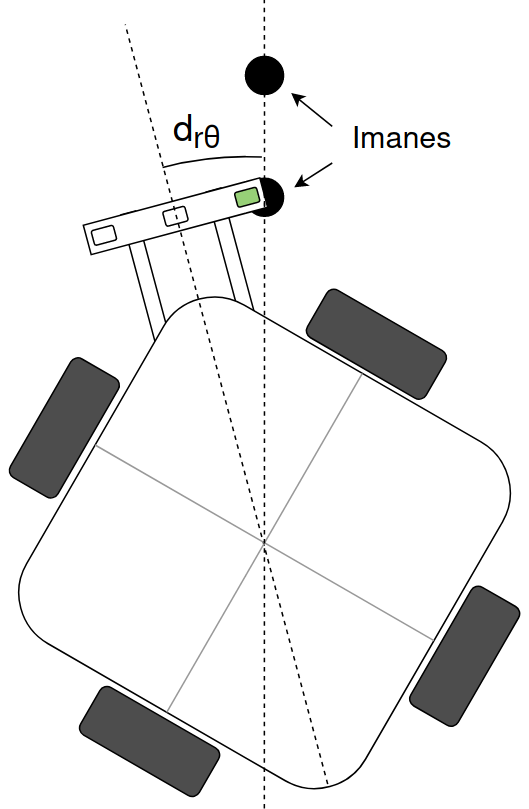
\includegraphics[width=0.4\linewidth]{images/robot_desplazamiento_angular_toca_iman.png}
    \caption{Escenario de detección de un imán}
    \label{fig:deteccionimanrobot}
\end{figure}

El enfoque propuesto es el de tener un acumulador que mide la distancia recorrida angularmente y ajusta la velocidad rotacional para compensar el desfase. Cada vez que se detecta un imán se suma o se resta un determinado valor de distancia angular de modo que el controlador intente llevarla a 0 nuevamente. Por ejemplo, si el robot detecta un desplazamiento hacia la derecha, se aumenta la velocidad rotacional hacia la izquierda.

El algoritmo de control opera de la siguiente manera:

\begin{enumerate}
    \item Los sensores magnéticos son monitoreados continuamente para detectar la presencia de imanes. Cada vez que se detecta un imán en alguno de los extremos, se actualiza un acumulador de distancia angular recorrida sumando o restando un valor determinado. Este valor depende de la distancia de los sensores al centro del robot y de la distancia entre los mismos.

    \item El objetivo es que el acumulador se mantenga en cero, lo que indicaría que el robot sigue la dirección de la trayectoria. El sistema de control ajusta las velocidades de las ruedas del robot en tiempo real en función al desplazamiento angular detectado.    
\end{enumerate}

Al realizar las pruebas, se lanzó al robot en distintas circunstancias, comenzando alineado con los imanes y comenzando con una desviación detectable. A medida que se avanzaron los ensayos se fue iterando sobre los coeficientes del seguidor de línea para compensar el error.

En una primera instancia, la implementación de la corrección del desplazamiento angular estaba dado por una velocidad fija. En las sucesivas experiencias, notamos que el robot a bajas velocidades se comportaba de un modo esperado y que a medida que se incrementaba la velocidad era menos estable. Es por ello que se cambió la velocidad constante por una que sea variable según la velocidad lineal del robot, es decir, ahora la compensación es adaptativa. De modo que a mayor velocidad lineal, mayor velocidad rotacional para realizar la compensación. Esto se debe a la inercia del robot, implicando que a mayor velocidad requiere mayor compensación para vencer el momento del mismo.

En la Figura \ref{fig:diagsecuencialinefollowmodcin} se detalla un diagrama de secuencia del funcionamiento del modelo cinemático compensado con el seguidor de línea.

\begin{figure}[H]
    \centering
    \hspace*{-1.25cm}
    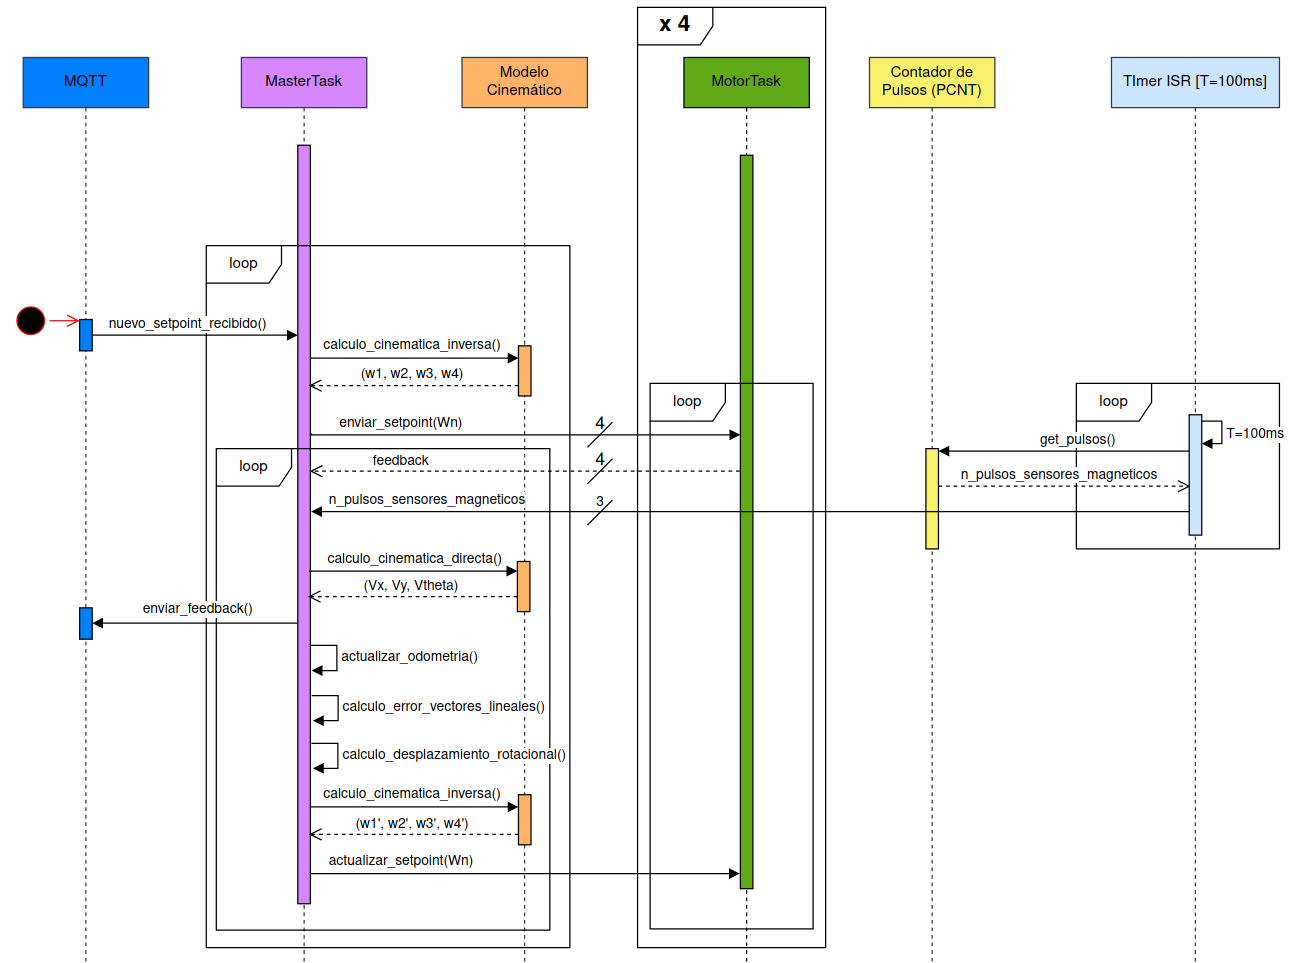
\includegraphics[width=1.2\linewidth]{images/diag_secuencia_seguidor_linea_magnetica_modelo_cinem_compensado.png}
    \caption{Diagrama de secuencia del seguidor de linea con el Modelo Cinemático}
    \label{fig:diagsecuencialinefollowmodcin}
\end{figure}


\subsection{Testing y pruebas}

Las pruebas realizadas en esta iteración parten del prototipo logrado en la iteración anterior.

\begin{testtableformat}
    \hline \rowcolor{test_header_color}
        Test ID             & TC\_02\_00 \\
    \hline
        Tipo de test        & Test de integración \\
    \hline
        Objeto de prueba    & Modelo Cinemático \\
    \hline
        Requerimiento       & RF4 - RF5 \\
    \hline
        Nombre              & Modelo Cinemático con compensación en línea recta \\
    \hline
        Descripción         & Comprobar que el Modelo Cinemático compensa adecuadamente las velocidades de las ruedas según un setpoint en línea recta \\
    \hline
        Precondición        & PRECOND\_B \\
    \hline
        Pasos del test      & \begin{enumerate}
                                \item Enviar al robot un setpoint con distancia entre [50cm $\sim$ 400cm] y velocidad lineal entre $\pm$[0.25m/seg $\sim$ 0.75m/seg]
                                \item Verificar que el robot recorre el vector dado a lo largo de la distancia determinada y que su movimiento es compensado
                                \item Repetir desde el paso 1) con diferentes valores
                            \end{enumerate} \\
    \hline
        Resultado esperado  & El robot se mueve en línea recta en la dirección del vector dado por $V_x$ y $V_y$. Debe ser notable la mejora en la estabilidad del vector a realizar. \\
    \hline
        Resultado obtenido  & Se observa que el robot mejora sustancialmente el desempeño al realizar la trayectoria. \\
    \hline
        Observaciones       & - \\
    \hline
\end{testtableformat}


\begin{testtableformat}
    \hline \rowcolor{test_header_color}
        Test ID             & TC\_02\_01 \\
    \hline
        Tipo de test        & Test de integración \\
    \hline
        Objeto de prueba    & Seguidor de línea magnética - Modelo Cinemático \\
    \hline
        Requerimiento       & RF5 \\
    \hline
        Nombre              & Compensación de linea magnética \\
    \hline
        Descripción         & Verificar que el robot compensa su trayectoria al comenzar centrado en la línea de imanes \\
    \hline
        Precondición        & PRECOND\_C \\
    \hline
        Pasos del test      & \begin{enumerate}
                                \item Colocar al robot centrado respecto a la línea de imanes
                                \item Enviar al robot un setpoint con distancia entre [50cm $\sim$ 400cm] y velocidad lineal entre $\pm$[0.25m/seg $\sim$ 0.75m/seg]
                                \item Verificar que el robot recorre el vector dado a lo largo de la distancia determinada, que el Modelo Cinemático compensa el movimiento y que al detectar un imán en un lateral se corrige la orientación del robot
                                \item Repetir desde el paso 1) con diferentes valores
                            \end{enumerate} \\
    \hline
        Resultado esperado  & El robot se mantiene dentro de los límites de la línea magnética \\
    \hline
        Resultado obtenido  & El robot logra mantenerse centrado con la línea de imanes. Se observa en varias ocasiones que el robot toca un imán, a lo que el robot aplica una velocidad rotacional contraria para centrarlo \\
    \hline
        Observaciones       & - \\
    \hline
\end{testtableformat}


\begin{testtableformat}
    \hline \rowcolor{test_header_color}
        Test ID             & TC\_02\_02 \\
    \hline
        Tipo de test        & Test de integración \\
    \hline
        Objeto de prueba    & Seguidor de línea magnética  - Modelo Cinemático \\
    \hline
        Requerimiento       & RF5 \\
    \hline
        Nombre              & Compensación de linea magnética \\
    \hline
        Descripción         & Verificar que el robot compensa su trayectoria al comenzar tocando un imán \\
    \hline
        Precondición        & PRECOND\_C \\
    \hline
        Pasos del test      & \begin{enumerate}
                                \item Colocar al robot descentrado respecto a la línea de imanes y de modo que se detecte un imán al inicio
                                \item Enviar al robot un setpoint con distancia entre [50cm $\sim$ 400cm] y velocidad lineal entre $\pm$[0.25m/seg $\sim$ 0.75m/seg]
                                \item Comprobar que al iniciar corrige su trayectoria de inmediato y que luego el robot se mantiene centrado a lo largo de la línea magnética, compensando con el Modelo Cinemático y al detectar imanes
                                \item Repetir desde el paso 1) con diferentes valores
                            \end{enumerate} \\
    \hline
        Resultado esperado  & El robot corrige el desfase y vuelve a posicionarse dentro de los límites de la línea \\
    \hline
        Resultado obtenido  & El robot logra mantenerse centrado con la línea. Se observa que al tocar un imán se aplica una velocidad rotacional contraria para centrarlo \\
    \hline
        Observaciones       & - \\
    \hline
\end{testtableformat}


\begin{testtableformat}
    \hline \rowcolor{test_header_color}
        Test ID             & TC\_02\_03 \\
    \hline
        Tipo de test        & Test de sistema \\
    \hline
        Objeto de prueba    & Comunicación inalámbrica - PID - Modelo cinemático compensado - Odometría - Seguidor de línea magnética \\
    \hline
        Requerimiento       & RF1 - RF2 - RF3 - RF4 - RF5 - RF6 \\
    \hline
        Nombre              & Prueba de sistema integrado \\
    \hline
        Descripción         & Comprobar que el robot realiza trayectorias en una dirección y longitud determinadas \\
    \hline
        Precondición        & PRECOND\_C \\
    \hline
        Pasos del test      & \begin{enumerate}
                                \item Enviar al robot un setpoint con distancia entre [50cm $\sim$ 400cm] y velocidad lineal entre $\pm$[0.25m/seg $\sim$ 0.75m/seg]
                                \item Comprobar que el robot se mantiene centrado a lo largo de la línea magnética y que es compensado por el Modelo Cinemático. Además debe reportar mediciones de velocidad y distancia
                                \item Repetir desde el paso 1) con diferentes valores
                            \end{enumerate} \\
    \hline
        Resultado esperado  & El robot responde correctamente al vector y la distancia establecida, reporta información de mediciones de velocidad y distancia \\
    \hline
        Resultado obtenido  & El robot realiza las trayectorias de manera acorde dentro de los límites observados en las pruebas unitarias y de integración. Se logra recolectar la información enviada por el robot \\
    \hline
        Observaciones       & Se probó hasta recorridos de 4 metros por limitaciones de espacio. \\
    \hline
\end{testtableformat}

\subsection{Resultados}

En el presente proyecto, se lograron avances significativos respecto al prototipo funcional desarrollado en la etapa anterior. Uno de los principales logros fue la implementación exitosa de compensaciones en varios niveles del sistema de control, lo cual permitió optimizar el rendimiento global del sistema. Estas compensaciones del modelo cinemático y de un seguidor de línea contribuyeron a mejorar la precisión y la estabilidad en condiciones de operación variables, reduciendo de manera notable los márgenes de error detectados previamente.

Asimismo, se llevaron a cabo pruebas exhaustivas que validaron la robustez del sistema mejorado, evidenciando un incremento en su capacidad para adaptarse a distintos escenarios operativos.

\begin{figure}[H]
    \centering
    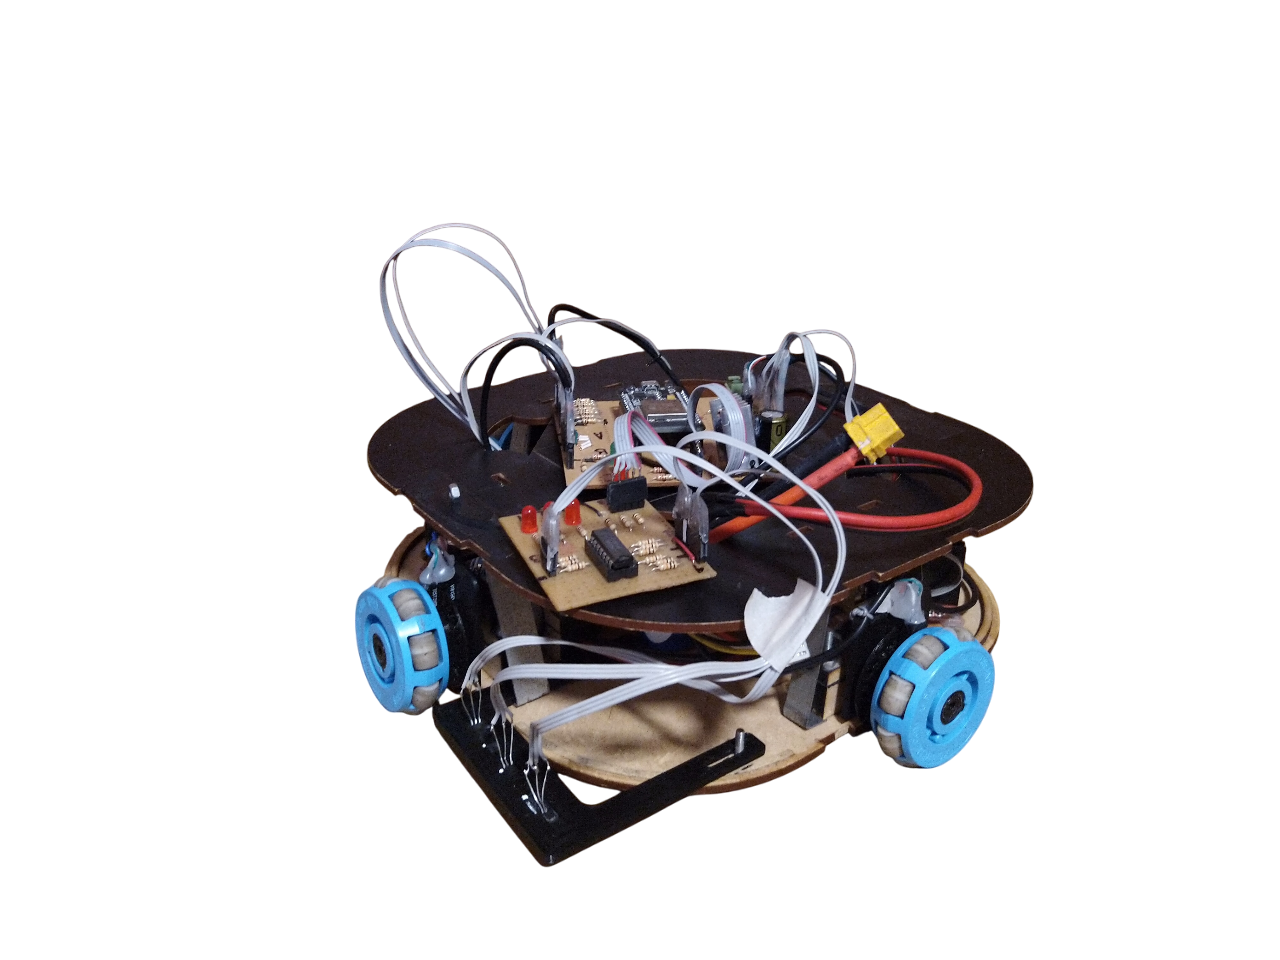
\includegraphics[trim={0 2cm 0 7.5cm}, clip, width=1.1\linewidth]{images/prototipo_robot_con_sens_mag.png}
    \caption{Prototipo del robot con seguidor de linea}
    \label{fig:prototiporobotlinef}
\end{figure}

\subsection{Riesgos superados}

Dado el desarrollo de esta iteración, se logro avanzar sobre el riesgo RI-03 y RI-01 por demostrar que los componentes elegidos aun son viables para escalar el proyecto pero existe lugar para mayor aprovechamiento de los mismos.

Por otra parte, se trabajó en superar el riesgo RI-02 por lograr una comunicación efectiva entre los componentes del sistema y se supera en parte el riesgo RI-05 al ser los nuevos componentes agregados de alta disponibilidad.

\begin{center} \begin{tabular}{|c|c|}
    \hline
        ID & Riesgo \\
    \hline
        RI-01 & Incompatibilidad o avería de componentes \\
    \hline
        RI-02 & Intercomunicación de componentes ineficiente o ineficaz \\
    \hline
        RI-03 & Prestaciones insuficientes de componentes \\
    \hline
        RI-05 & Dificultad en conseguir determinados componentes. \\
    \hline
\end{tabular} \end{center}

\subsection{Conclusiones}

Con la realización de esta iteración, obtuvimos que la implementación de compensaciones en el sistema de control marcó un hito al optimizar aspectos clave como la precisión, la estabilidad y la adaptabilidad del sistema frente a distintas condiciones de operación. Estos logros no solo demuestran la efectividad de las estrategias propuestas, sino que también refuerzan la importancia de un enfoque continuo hacia la mejora y la innovación del proyecto.


\newpage
\section{Iteración 3: Modelo del mapa e interfaz}

\subsection{Introducción}
Durante el desarrollo de la iteración anterior se logró construir y optimizar el robot, integrando compensaciones en el sistema de control para mejorar su estabilidad y precisión operativa.

En la presente iteración se busca avanzar aún más en las capacidades del robot mediante el modelado del espacio en el que operará, esto mediante la creación de una representación del mapa de su entorno.

Además, se buscará desarrollar una interfaz de usuario que facilitará la interacción y monitoreo del sistema.

\subsection{Requerimientos}
En esta iteración abordaremos los siguientes requerimientos funcionales:

\begin{center} \begin{tabular}{|c|c|}
\hline
    ID & Descripción \\
\hline
    RF7 & Debe existir un modo de calcular trayectorias automáticamente. \\
\hline
    RF10 & Debe existir una interfaz de usuario para control y monitoreo. \\
\hline
\end{tabular} \end{center}

Por otra parte, los requerimientos no funcionales que trataremos son:

\begin{center} \begin{tabular}{|p{0.10\linewidth}|p{0.65\linewidth}|}
\hline
    ID & Descripción \\
\hline
    RNF1 & Debería tener tiempos de respuesta aceptables para el buen funcionamiento del sistema de control. \\
\hline
    RNF2 & El software debería contar con pruebas unitarias y de integración. \\
\hline
    RNF4 & El código debería contar con documentación.\\
\hline
\end{tabular} \end{center}

\subsection{Desarrollo}

\subsubsection{Modelado del mapa}

Para empezar, es crucial tener un diseño inicial del entorno donde se moverá el robot, que incluya paredes, obstáculos y puntos de interés. Dado que el robot solo se mueve en líneas rectas, este proceso puede ser más sencillo en comparación con robots que tienen libertad de movimiento en todas las direcciones.

El siguiente paso fue la creación del modelo del mapa, donde se divide el entorno en una cuadrícula (grid) y cada celda se marca como libre, ocupada, obstáculo o borde. Cada celda es cuadrada y tiene un lado de $0.5[m]$. Además de ello, el control de movimiento del robot debe estar alineado con los ejes de la grid, y se utilizan algoritmos como A* o Dijkstra para planificar rutas en línea recta.

Mientras el robot se mueve y los sensores recopilan datos, las celdas de la grid se deben actualizar continuamente, indicando si están libres u ocupadas. Esta actualización constante del mapa es esencial para mantener la precisión y eficiencia en el mapeo. Al mismo tiempo, es importante validar que el mapa generado es preciso y coincide con el entorno real.

Debajo se muestra el modelo del mapa que consideramos para el proyecto. Decidimos que los colores de referencia son:

\begin{itemize}
    \item Rojo: borde o límite del mapa
    \item Blanco: obstáculo
    \item Gris: celda ocupable libre
    \item Otro: robot ocupando una celda
\end{itemize}

El punto verde en la imagen de debajo simboliza el origen efectivo del mapa, es la primera celda ocupable del mapa. Además en el centro existe un obstáculo que torna a esa celda no ocupable. Las coordenadas representadas en el mapa son coordenadas ordinales de las celdas, al realizar la odometría se toma el valor de medición en metros. Por lo que si el robot está en la celda $(3, 2)$, la posición reportada por la odometría será $(1.5, 1.0)$, dado que cada celda tiene $0.5[m]$ de lado.

\begin{figure}[H]
    \centering
    \includegraphics[width=0.8\linewidth]{images/modelo_del_mapa.png}
    \caption{Modelo del mapa}
    \label{fig:modelomapa}
\end{figure}


\subsubsection{Path Finder}

Dentro de los algoritmos de planificación de trayectorias, elegimos utilizar A* por su gran eficiencia en encontrar el camino mas corto y ser ampliamente conocido y estudiada su efectividad. Su objetivo es encontrar el camino más corto entre dos puntos en un mapa combinando las ventajas de los algoritmos de búsqueda de coste uniforme y heurística. \cite{sariffpathplan} \cite{cuevaspathfinding}

$A*$ funciona evaluando cada celda del mapa utilizando una función de costo:

$$ f(n) = g(n) + h(n) $$

Donde $g(n)$ es el costo acumulado desde el punto inicial hasta la celda actual, y $h(n)$ es una heurística que estima el costo restante desde la celda actual hasta el destino. La heurística debe ser admisible, lo que significa que nunca sobreestima el costo real para garantizar que el algoritmo encuentre el camino más corto.

El proceso comienza con la celda inicial, que se agrega a una lista abierta (open list) de celdas por explorar. En cada paso, el algoritmo selecciona la celda con el valor $f(n)$ más bajo de la lista abierta y la mueve a una lista cerrada (closed list) de celdas ya exploradas. Luego, evalúa las celdas vecinas de la celda actual. Si una celda vecina no está en la lista cerrada y no hay una ruta mejor a esa celda en la lista abierta, se actualizan sus valores de $g$, $h$ y $f$, y se agrega a la lista abierta.

Este proceso se repite, seleccionando y evaluando celdas hasta que se alcanza la celda destino. A medida que se avanza, $A*$ construye el camino más corto de regreso desde el destino hasta el origen siguiendo los valores de $g$. La clave del éxito del algoritmo $A*$ es su capacidad para equilibrar de manera eficiente el costo acumulado $g(n)$ y la heurística $h(n)$, permitiéndole encontrar rutas óptimas de manera efectiva.

La eficiencia de $A*$ depende en gran medida de la heurística utilizada. La heurística más común es la distancia de Manhattan para movimientos en una cuadrícula ortogonal, o la distancia euclidiana para movimientos en cualquier dirección. En nuestro caso la técnica mas conveniente es utilizar la distancia de Manhattan.



\subsubsection{Interfaz de usuario}

En la pantalla principal de la interfaz se muestra un mapa interactivo del entorno, con una cuadrícula que representa el mapa. La interfaz muestra información en tiempo real sobre la celda actual en la que se ubica el robot en el mapa, actualizándose conforme el robot se desplaza. Además, se proporciona información sobre la dirección de movimiento.

El usuario comienza estableciendo los puntos de inicio y destino haciendo click en las celdas disponibles. Cuando se da la orden de inicio, se calcula la ruta óptima y se envían los comandos al robot. Paso seguido, la interfaz muestra continuamente en tiempo real la celda del robot y se envían los comandos de movimiento hacia las celdas subsiguientes.

\begin{figure}[H]
    \centering
    \includegraphics[width=0.85\linewidth]{images/interfaz_de_usuario}
    \caption{Interfaz de usuario}
    \label{fig:interfazusuario}
\end{figure}



\input{iteraciones_desarrollo/iteracion_3/diseño_pista}

\subsection{Testing y pruebas}

\begin{testtableformat}
    \hline \rowcolor{test_header_color}
        Test ID             & TC\_03\_00 \\
    \hline
        Tipo de test        & Test unitario \\
    \hline
        Objeto de prueba    & Calculador de trayectorias \\
    \hline
        Requerimiento       & RF7 \\
    \hline
        Nombre              & Cálculo de trayectorias en un mapa con obstáculos, trayectoria resoluble \\
    \hline
        Descripción         & Calcular la secuencia de coordenadas a seguir para llegar a un punto A a un punto B del mapa, con obstáculos dispuestos de modo que existe al menos una trayectoria posible \\
    \hline
        Precondición        & PRECOND\_E \\
    \hline
        Pasos del test      & \begin{enumerate}
                                \item Enviar al PathFinder una coordenada origen y una destino de modo que exista un camino soluble entre ellas
                                \item Verificar que la salida del PathFinder consiste en la secuencia de coordenadas del mapa que se deben visitar para llegar del origen al destino
                                \item Repetir desde el paso 1) con diferentes valores
                            \end{enumerate} \\
    \hline
        Resultado esperado  & Se obtiene la secuencia adecuada para los puntos dados y se cumple la restricción de solo movimientos horizontales o verticales \\
    \hline
        Resultado obtenido  & La secuencia de coordenadas calculadas se corresponden a las más óptimas para cada par de puntos y se cumple la restricción de movimiento \\
    \hline
        Observaciones       & - \\
    \hline
\end{testtableformat}


\begin{testtableformat}
    \hline \rowcolor{test_header_color}
        Test ID             & TC\_03\_01 \\
    \hline
        Tipo de test        & Test unitario \\
    \hline
        Objeto de prueba    & Calculador de trayectorias \\
    \hline
        Requerimiento       & RF7 \\
    \hline
        Nombre              & Cálculo de trayectorias en un mapa con obstáculos, trayectoria irresoluble \\
    \hline
        Descripción         & Calcular la secuencia de coordenadas a seguir para llegar a un punto A a un punto B del mapa, con obstáculos dispuestos de modo que no existe ninguna trayectoria posible \\
    \hline
        Precondición        & PRECOND\_F \\
    \hline
        Pasos del test      & \begin{enumerate}
                                \item Enviar al PathFinder una coordenada origen y una destino de modo que no exista camino posible entre ellas
                                \item Verificar que la salida del PathFinder es un error
                                \item Repetir desde el paso 1) con diferentes valores
                            \end{enumerate} \\
    \hline
        Resultado esperado  & Se obtiene un mensaje de error informando que no existe trayectoria posible \\
    \hline
        Resultado obtenido  & El error se presenta solo cuando se define el mapa de modo que entre un punto A y un punto B no existe camino posible \\
    \hline
        Observaciones       & - \\
    \hline
\end{testtableformat}


\subsection{Resultados}
Uno de los principales resultados fue el desarrollo de una interfaz de usuario simple que facilita el control y la supervisión del robot. Aparejado con ello, se introdujo un calculador de trayectorias que optimiza los movimientos del robot en el espacio modelado.

Por último se logró implementar una pista fabricada con madera MDF, con imanes integrados, la cual garantiza estabilidad y uniformidad en las pruebas del sistema. Esta pista, además, fue modelada y representada tanto en el mapa desarrollado como en la interfaz, manteniendo la coherencia del entorno del robot.


\begin{figure}[H]
    \centering
    \includegraphics[width=1\linewidth]{images/robot_en_pista_final.png}
    \caption{Robot en la pista con imanes}
    \label{fig:robotpistaconimanes}
\end{figure}

\subsection{Riesgos superados}
En esta iteración pudimos demostrar que los nuevos componentes integrados al sistema interactúan efectivamente con los ya desarrollados en las iteraciones previas, por lo que se avanza sobre el riesgo RI-02.

Del mismo modo, se supera en parte el riesgo RI-05 por tener una alta disponibilidad de servicios de corte láser en MDF y los imanes son muy accesibles.

\begin{center}
\begin{tabular}{|c|c|} 
    \hline
        ID & Riesgo \\
    \hline
        RI-02 & Intercomunicación de componentes ineficiente o ineficaz \\
    \hline
        RI-05 & Dificultad en conseguir determinados componentes. \\
    \hline
\end{tabular}
\end{center}

\subsection{Conclusiones}

En esta iteración del proyecto se han alcanzado avances fundamentales, como la inclusión de un calculador de trayectorias que optimiza los movimientos del robot dentro de la pista, marcando un avance fundamental para su rendimiento.

Asimismo, se avanzó con la creación de una interfaz de usuario funcional y sencilla permitiendo un control y monitoreo más efectivo del sistema. 

Por su parte, la implementación de una pista de superficie consistente que representa el espacio de movimiento del robot ha proporcionado un entorno operacional estable, ideal para las pruebas del robot.

En definitiva, el proyecto avanza hacia su consolidación como una solución robusta, eficiente y adaptable.

\newpage
\section{Iteración 4: Red de Petri y monitor}

\subsection{Introducción}
El control de navegación de un robot omnidireccional es un desafío complejo que requiere la coordinación de múltiples tareas, como la planificación de trayectorias, el eludir obstáculos y la ejecución de movimientos precisos. Las redes de Petri son una herramienta matemática y gráfica que permite modelar, analizar y controlar sistemas discretos y concurrentes, lo que las hace particularmente útiles para gestionar la navegación de robots en entornos dinámicos. A continuación se establece la relación entre el control de navegación y las redes de Petri.

\subsection{Requerimientos}

En esta iteración abordaremos los siguientes requerimientos funcionales:

\begin{center}
    \begin{tabular} {
        | >{\centering\arraybackslash}m{1cm}
        | >{\centering\arraybackslash}m{13cm} |}
        \hline \rowcolor{test_header_color}
            ID & Descripción \\
        \hline
            RF4 & El robot debe poder realizar trayectorias en línea recta y curvas. \\
        \hline
            RF6 & El robot debe recibir y enviar información mediante comunicaciones inalámbricas. \\
        \hline
            RF8 & Debe poder ubicarse al robot en el plano de forma precisa. \\
        \hline
    \end{tabular}
\end{center}

   Por otra parte, el requerimiento no funcional que abordaremos es:

\begin{center}
    \begin{tabular} {
        | >{\centering\arraybackslash}m{1cm}
        | >{\centering\arraybackslash}m{13cm} |}
        \hline \rowcolor{test_header_color}
            ID & Descripción \\
        \hline
            RNF1 & Debería tener tiempos de respuesta aceptables para el buen funcionamiento del sistema de control. \\
        \hline
    \end{tabular}
\end{center}

\subsection{Desarrollo}

\subsubsection{Modelo del mapa con Red de Petri}

Como este trabajo tiene por objetivo el control, seguimiento del comportamiento y modelado de un sistema compuesto por una flota de robots donde cada uno tiene que seguir una trayectoria definida y calculada previamente utilizando el algoritmo $A*$ determinando el camino más corto hacia su destino. Teniendo esto en mente es necesaria la implementación de un método para evitar los problemas inherentes en los sistemas multi-robot: las colisiones entre los robots y los bloqueos del sistema, haciendo que algunos robots no puedan terminar su trayectoria y por lo tanto entorpecer todo el sistema.

Al tener el conjunto de trayectorias definidas para cada robot, se modela el sistema y el mapa mediante el uso de Redes de Petri, que no son más que representaciones matemáticas con una representación gráfica de un sistema de eventos discretos. El entorno en el cual se mueven los robots se considera particionado el mapa en regiones (celdas) y cada región del mapa se modela como una plaza en la Red de Petri. Para evitar las colisiones entre los robots, se establecen regiones con capacidad finita (recursos), donde, no pueden pasar por ellas mas robots de los recursos definidos. \cite{mahulea2020multi}

Si más de un robot desea pasar por la misma región en donde ya se encuentra posicionado un robot, el segundo debe esperar que la celda se libere y por lo tanto es necesario añadir lugares de espera. Estos lugares pueden conducir a bloqueos en la Red de Petri, ocasionando que los robots no lleguen a su destino. Los bloqueos se pueden caracterizar en la Red de Petri utilizando algunos elementos estructurales denominados sifones. Controlando que estos elementos no se vacíen, la red no se bloquea.

\begin{figure}[H]
   \centering
   \includegraphics[trim={1.35cm 0 0.9cm 1.5cm}, clip, width=0.6\linewidth]{images/mapa_py.png}
   \caption{Representación de un mapa en Python}
   \label{fig:mapa_py}
\end{figure}

La capacidad de las regiones, es decir, el número de robots que pueden estar simultáneamente en un lugar, se modela mediante los lugares de recursos, a los cuales se les asigna una marca (recurso), cuando el robot entra en una región específica y que se libera cuando el robot deja esa región.

Como ya se ha comentado la aplicación inmediata de los algoritmos implementados para este trabajo es la creación de una plataforma para el control de un sistema multi-robot con el objetivo de evitar colisiones entre los robots móviles. Sin embargo, se puede aplicar a cualquier sistema que sea modelable mediante redes de Petri. Por ello este proyecto tiene trascendencia en todas las áreas del control mediante sistemas de eventos discretos.

Antes de la implementación de uno de estos procesos, es muy importante modelarlo con un sistema discreto, comprobar su funcionamiento y corregirlo si hace falta. Las redes de Petri son una herramienta ampliamente utilizada cuando se trata de sistemas concurrentes, y como en cualquier otro sistema con recursos compartidos pueden aparecer bloqueos, así que este proyecto puede servir para resolver estos bloqueos haciendo el correcto uso de los recursos compartidos y gestionando de forma adecuada su utilización.

Un paso a realizar para obtener el modelo discreto del sistema multi-robot es dividir el mapa en regiones, ya que cada región del mapa se modelará como un lugar en el modelo de la red de Petri o como un nodo en el modelo de un autómata finito determinista. Para resolver el problema mencionado de dividir el mapa en regiones, se utiliza el método de la \textit{Descomposición en celdas}. Este método consiste en dividir las zonas sin obstáculos del plano mediante un cuadrado. Esto se puede ver claramente en la imagen anterior donde las celdas en color gris son las regiones disponibles o habitables por el robot mientras que las celdas rojas representan los límites del mapa.

Una vez descompuesto el mapa en regiones, queda calcular las trayectorias de cada robot para saber porque regiones ha de pasar para alcanzar de la forma más óptima el objetivo prefijado. Las trayectorias son obtenidas de forma automática a partir de algoritmos de cálculo de trayectorias individualmente para cada uno de los robots ignorando al resto de ellos utilizando algoritmos de búsqueda de caminos mínimos en grafos, o también pueden calcularse mediante algoritmos de planificación multi-robot ignorando las posibles colisiones entre los mismos utilizando programación matemática y modelos de tipo redes de Petri. En nuestro caso optamos por utilizar el algoritmo de $A*$, el cual busca el camino más corto para el robot hacía su destino último.

Si los dos robots individualmente siguen sus propias trayectorias, estos pueden colisionar (plazas ocupadas) ya que sus trayectorias pasan por esas regiones que tienen capacidad unitaria (un solo robot puede haber dentro de ellas en cualquier momento). Para evitar las posibles colisiones, se introducen modos de espera, es decir, se impone que por estas regiones no pueda pasar más de un robot al mismo tiempo, de modo que el segundo en llegar a esas regiones deberá esperar a que el primero salga de esa área.

Para sostener este concepto de regiones con capacidad limitada a las redes de Petri, se introducen lugares adicionales, a los que se les llama lugares de capacidades o de recursos compartidos. Estos lugares contienen inicialmente tantas marcas como capacidad tenga la región, en este caso se asignaran recursos con una marca a los lugares que corresponden a regiones con capacidad unitaria. Esta marca se utiliza para disparar la transición de entrada al lugar con capacidad limitada, y cuando el robot abandona esa zona, la transición de salida de ese lugar libera la marca para que vuelva a ser utilizada por el otro robot. Utilizando este concepto para todos los lugares con capacidad finita, la red quedaría como la siguiente.

\begin{figure}[H]
   \centering
   \includegraphics[width=0.8\linewidth]{images/rdp_no_grid.png}
   \caption{Representación del mapa en Python en una red de Petri}
   \label{fig:rdp_no_grid}
\end{figure}

Cabe destacar, que conforme va evolucionando el sistema y los robots se van moviendo de una región a otra, el marcado de la red va cambiando hasta que finalmente cuando un robot termina su trayectoria, la marca vuelve al lugar de reposo, sin embargo, el modelo de  red de Petri no podría volver a ser usado para supervisar el movimiento hasta que el robot sea colocado de nuevo en la posición de inicio del modelo.

Esta simple idea lo que hace es generar modos de espera de modo que nunca puedan coincidir en una región con capacidad restringida más de un robot. De modo que escogiendo correctamente estas regiones en las zonas donde las trayectorias de los robots coinciden, se pueden evitar las colisiones entre robots. Esto es debido a que los recursos compartidos producen modos de espera.

\paragraph{Transformación de un mapa a una red de Petri} \mbox{} \vspace{8pt}

Dentro del programa en Python existe una clase que se encarga de realizar esta transformación, el proceso consiste en definir la estructura que va a tener el mapa, es decir, cuáles van a ser sus espacios habitables y cuáles los límites. Entendiendo cómo límites a las paredes por fuera de la superficie de desplazamiento (su perímetro), y a los obstáculos que pueden existir dentro del mapa (paredes interiores, columnas, objetos, etc). Esto se hace en un archivo de texto que va a ser leído e interpretado por el algoritmo para luego ser convertido en una red de Petri.

\begin{figure}[H]
   \centering
   \includegraphics[width=0.5\linewidth]{images/map_definition_matriz.png}
   \caption{Matriz que define el mapa y sus elementos para el programa en Python}
   \label{fig:map_definition}
\end{figure}

La figura \ref{fig:map_definition} muestra el contenido del archivo de texto definido como una matriz de elementos donde, los números $-1$ representan los límites del mapa, los números $1$ los obstáculos y por último los números $0$ los espacios habitables.

El contenido del archivo que se muestra en la imagen anterior es el interpretado por el algoritmo y transformado. De este archivo se obtienen dos definiciones fundamentales para representar de forma correcta y suficiente a la red de Petri. Por un lado la matriz de incidencia, la cual nos describe la relación que existe entre las plazas y las transiciones de la red, es decir, como va a ser el movimiento de los tokens a medida que se disparen las transiciones, y por el otro lado el marcado inicial de la red, es decir, la distribución de los tokens en la red cuando todavía no se disparó ninguna transición. Cómo nosotros buscamos que la red cumpla ciertas condiciones para su adecuado comportamiento (por ejemplo no ser bloqueante), añadimos un lugar de recurso y un lugar de ocupación para celda habitable del mapa, es por ello que la imagen \ref{fig:rdp_no_grid} luce de esa manera.

Todo el proceso de transformación se encuentra descrito en la siguiente imagen, desde la lectura del archivo donde se define la estructura del mapa, pasando por su conversión a las matrices de incidencia y marcado, y por último en cómo el monitor toma esa red de Petri para decidir sobre el avance de los robots en el mapa.

\begin{figure}[H]
   \centering
   \includegraphics[width=1.0\linewidth]{images/diagrama_clase_monitor.jpg}
   \caption{Diagrama de alto nivel de la transformación de un mapa a una red de Petri}
   \label{fig:mapa_to_rdp}
\end{figure}

\subsubsection{Concurrencia en Python}

Python ofrece diversas formas de manejar la concurrencia, permitiendo que múltiples tareas se ejecuten de manera simultánea. Las principales herramientas para lograrlo incluyen hilos, procesos y asincronía. Sin embargo, la concurrencia en Python está influenciada y controlada por el \textit{Global Interpreter Lock (GIL)}, el cual impide que múltiples hilos ejecuten código Python puro en paralelo dentro de un mismo proceso. Esto influye en su rendimiento ya que todos los hilos, excepto en algunas ocasiones como en las operaciones de entrada/salida, se van a ejecutar en un solo procesador y por lo tanto no se aprovecha todo el potencial de un computador. \cite{lanaro2017python}

El módulo threading permite la ejecución concurrente de tareas dentro del mismo proceso, pero debido al GIL, los hilos no pueden aprovechar múltiples núcleos para realizar cómputo intensivo. Aun así, el threading sigue siendo útil, y sobre todo en el enfoque que estamos tomando para su utilización. Aclarando, los hilos pueden aprovechar el tiempo en el que un proceso está inactivo esperando información, permitiendo la ejecución de otras tareas en paralelo.

Por otro lado, cuando se requiere ejecutar tareas que demandan un alto uso de CPU, la mejor alternativa es el multi procesamiento, que crea procesos independientes con su propio intérprete de Python, evitando la restricción del \textit{GIL} y permitiendo una ejecución realmente paralela.

Teniendo en cuenta que este proyecto está pensado para que escale en cantidad de robots, y se pueda controlar una flota de ellos, se ha optado por utilizar threading debido a que cada hilo va a representar un robot, cuya gestión va a estar coordinada a través del monitor basado en una Red de Petri. Dado que los robots no requieren cómputo intensivo, sino que dependen principalmente de operaciones de I/O y sincronización de eventos, threading resulta adecuado a pesar de las limitaciones del GIL.

Para garantizar un control ordenado de los hilos, se ha implementado un mecanismo de sincronización mediante Lock, permitiendo bloquear el hilo de un robot cuando este no puede avanzar y continuar con los demás. Este enfoque asegura una ejecución eficiente dentro del marco definido por la red de Petri, optimizando el flujo de trabajo sin afectar la estabilidad del sistema.

\subsubsection{Monitor} \mbox{} \vspace{1pt}

La manera en que controlamos la ocupación de los espacios en el mapa, es decir, cómo evoluciona la trayectoria de cada robot es mediante el disparo de un Monitor implementado en Python. Este es el va a controlar, guiar y realizar la toma de decisiones para que cada robot pueda seguir su trayectoria sin interrumpir a los demás y por lo tanto no bloquear todo el sistema.

Para poder guiar a cada robot en su trayectoria, cada uno va a estar representado por un hilo lógico en el programa en Python. Más precisamente cuando existe un robot en el mundo real y se realiza el proceso de sincronización con el software, este va a crear un objeto (representación de un ente en la Programación Orientada a Objetos) el cual va a contener un conjunto de métodos implementados y entre ellos, la creación de un hilo en Python.

A su vez definimos cuál va a ser el punto de inicio y el punto final, es decir el comienzo del recorrido y el final del mismo, y el mapa es un modelo discreto representado por una Red de Petri. Podemos determinar cuales van a ser la plazas que el robot va a ocupar en un preciso momento y las transiciones que se van a disparar para que este pueda llegar a su destino. Con todos estos elementos le damos al monitor las herramientas para realizar su trabajo y efectuar los métodos que le permitan modificar el marcado de la Red de Petri.

\paragraph{Cola de cortesía} \mbox{} \vspace{5pt}

La manera en que el Monitor ejerce el control de la exclusión mutua dentro de la Red de Petri es mediante el uso de colas, entonces, cuando un hilo (robot) está dentro del monitor y aparece otro hilo que intenta ejecutar otro o el mismo procedimiento, el acceso al Monitor se bloquea e inserta el segundo hilo en una cola de cortesía usando una política FIFO. Cuando el primer hilo abandona el monitor, el segundo hilo (que se encuentra en el primer lugar de la cola) es el seleccionado por el Monitor para ejecutar sus tareas. Si la cola está vacía entonces el Monitor se encuentra libre y cualquier hilo que intente tomar el control de éste último podrá hacerlo sin intervención alguna.

\paragraph{Políticas} \mbox{} \vspace{5pt}

Así como mencionamos más arriba que hacemos uso de las colas del monitor para controlar la exclusión mutua, existe la posibilidad de que dos hilos (robots) intenten acceder a la misma plaza ya que su secuencia de disparos así lo determina. En ese caso vamos a tener que tomar una decisión de qué hilo es que va a lograr apoderarse de la plaza en primer lugar. Para esto hacemos uso de una Política definida por nosotros mismos, a partir de ella un hilo va a tener preferencia sobre otro.

Poniendo el caso en concreto de los robots que comparten un mapa, nos parece más acertada la idea de que un robot pueda terminar su recorrido de forma rápida y efectiva. Es por ello que cada robot va guardando el camino que va atravesando, es decir, las celdas por las cuales se desplazó y aumentando un contador interno. Este es el parámetro que se usa para determinar qué robot va a tener preferencia sobre otro, entonces, al momento de ocurrir un conflicto entre dos robots que intentan ocupar la misma celda, el Monitor va a evaluar que robot es el que tiene un mayor camino recorrido y elegirlo para ocupar el lugar en disputa.

\paragraph{Solución de conflictos entre robots} \mbox{} \vspace{5pt}

Acá representamos el posible conflicto que puede ocurrir cuando dos robots intentan ocupar el mismo lugar, como se representan en el mapa y su traducción en una Red de Petri.

\begin{figure}[H]
    \centering
    \includegraphics[width=0.7\linewidth]{images/conflicto_map.png}
    \caption{Representación de un conflicto entre dos robots que intentan pasar por la misma celda}
    \label{fig:conflicto_map}
\end{figure}

\begin{figure}[H]
    \centering
    \includegraphics[width=0.7\linewidth]{images/rdp_no_grid_conflicto.png}
    \caption{Representación del conflicto de la figura \ref{fig:conflicto_map} en una red de Petri}
    \label{fig:rdp_no_grid_conflicto}
\end{figure}

\begin{figure}[H]
    \centering
    \includegraphics[width=0.7\linewidth]{images/conflicto_map_solucionado.png}
    \caption{Resolución del conflicto de dos robots intentando pasar por la misma celda}
    \label{fig:conflicto_map_solucionado}
\end{figure}

\begin{figure}[H]
    \centering
    \includegraphics[width=0.7\linewidth]{images/rdp_no_grid_conflicto_solucionado.png}
    \caption{Resolución del conflicto entre los robots representado en una red de Petri y con el nuevo marcado de la red}
    \label{fig:rdp_no_grid_conflicto_solucionado}
\end{figure}

\paragraph{Funcionamiento del monitor} \mbox{} \vspace{10pt}

El funcionamiento del módulo del Monitor en Python queda representado en el siguiente Diagrama de secuencia.

\begin{figure}[H]
    \centering
    \includegraphics[width=1.0\linewidth]{images/diagrama_monitor.drawio.png}
    \caption{Diagrama de secuencia del monitor}
    \label{fig:diagrama_monitor}
\end{figure}

\subsection{Testing y pruebas}

Las pruebas que se realizaron para que efectivamente podamos determinar el correcto funcionamiento del Monitor, la gestión de la cola de cortesía y la resolución de conflictos mediante la aplicación de una Política fue con la ayuda de la Red de Petri sumamente conocida como Productor-Consumidor. Esta se tomó cómo referencia ya que permite evaluar los problemas de sincronización, concurrencia y gestión de los recursos, entonces, nos pareció un buen puntapié para validar el funcionamiento con un modelo conocido y sumamente usado. Cabe destacar que realizamos la simulación sobre esta red alrededor de $1M$ de disparos y por supuesto siempre validando el resultado de los $P\ invariantes$ y $T\ invariantes$.

\begin{figure}[H]
   \centering
   \includegraphics[width=0.9\linewidth]{images/rdp_prod_cons.png}
   \caption{Red de Petri productor-consumidor}
   \label{fig:rdp_prod_cons}
\end{figure}

Se plantearon los siguientes casos:

\begin{testtableformat}
   \hline \rowcolor{test_header_color}
       Test ID             & TC\_04\_00 \\
   \hline
       Tipo de test        & Test unitario \\
   \hline
       Objeto de prueba    & Disparar las transiciones sensibilizadas del Productor \\
   \hline
       Nombre              & Ejecución del productor \\
   \hline
       Descripción         & Realizar el disparo de las transiciones sensibilizadas del productor teniendo como máximo 3 (tres) tokens disponibles para producir\\
   \hline
       Precondición        & PRECOND\_D \\
   \hline
       Pasos del test      & \begin{enumerate}
                             \item Instanciar a la clase monitor con la red productor-consumidor
                             \item Obtener el vector de transiciones sensibilizadas 
                             \item Ejecutar un disparo de la transición sensibilizada 
                             \item Adquirir el marcado saliente y compararlo con un programa de análisis de redes de Petri 
                             \end{enumerate}\\
   \hline
       Resultado esperado  & El marcado en ambos casos debe coincidir \\
   \hline
       Resultado obtenido  & El marcado de la red obtenido por la clase monitor y el programa de análisis de redes de Petri son iguales, por lo tanto, se verifica su adecuado funcionamiento \\
   \hline
       Observaciones       & -\\
   \hline
\end{testtableformat}

\begin{testtableformat}
   \hline \rowcolor{test_header_color}
       Test ID             & TC\_04\_01 \\
   \hline
       Tipo de test        & Test unitario \\
   \hline
       Objeto de prueba    & Disparar las transiciones sensibilizadas del consumidor \\
   \hline
       Nombre              & Ejecución del consumidor \\
   \hline
       Descripción         & Realizar el disparo de las transiciones sensibilizadas del consumidor teniendo como máximo 3 (tres) recursos disponibles generados por el productor\\
   \hline
       Precondición        & PRECOND\_D \\
   \hline
       Pasos del test      & \begin{enumerate} 
                             \item Instanciar a la clase monitor con la red productor-consumidor 
                             \item Obtener el vector de transiciones sensibilizadas 
                             \item Ejecutar un disparo de la transición sensibilizada 
                             \item Adquirir el marcado saliente y compararlo con un programa de analisis de redes de petri 
                             \end{enumerate}\\
   \hline
       Resultado esperado  & El marcado en ambos casos debe coincidir \\
   \hline
       Resultado obtenido  & El marcado de la red obtenido por la clase monitor y el programa de análisis de redes de Petri son iguales, por lo tanto, se verifica su adecuado funcionamiento \\
   \hline
       Observaciones       & -\\
   \hline
\end{testtableformat}

\begin{testtableformat}
   \hline \rowcolor{test_header_color}
       Test ID             & TC\_04\_02 \\
   \hline
       Tipo de test        & Test unitario \\
   \hline
       Objeto de prueba    & Disparar una transición con política de decisión \\
   \hline
       Nombre              & Ejecución de una transición con política definida \\
   \hline
       Descripción         & En en el caso donde tanto el productor cómo el consumidor pueden disparar una transición, la idea es evaluar la política de la transición del consumidor para que tenga prevalencia sobre el productor ante una situación indeterminista \\
   \hline
       Precondición        & PRECOND\_E \\
   \hline
       Pasos del test      & \begin{enumerate} 
                             \item Instanciar a la clase monitor con la red productor-consumidor 
                             \item Generar una situación de equidad donde ambos recursos puedan disparar su transición 
                             \item Obtener el vector de transiciones sensibilizadas 
                             \item Evaluar la política de las transiciones sensibilizada y elegir cual disparar 
                             \item Ejecutar un disparo de la transición elegida 
                             \item Adquirir el marcado saliente y compararlo con un programa de análisis de redes de petri 
                             \end{enumerate}\\
   \hline
       Resultado esperado  & El marcado actual en ambos casos debe coincidir y la transición disparada debe ser la del consumidor \\
   \hline
       Resultado obtenido  & El marcado de la red obtenido por la clase monitor y el programa de análisis de redes de Petri son iguales, por lo tanto, se verifica su adecuado funcionamiento \\
   \hline
       Observaciones       & -\\
   \hline
\end{testtableformat}

\begin{testtableformat}
   \hline \rowcolor{test_header_color}
       Test ID             & TC\_04\_03 \\
   \hline
       Tipo de test        & Test integración \\
   \hline
       Objeto de prueba    & Realizar movimientos con el robot dentro del mapa, el robot sólo va a avanzar cuando la red de Petri haya hecho la solicitud de disparo y haya verificado que el robot no se encuentra bloqueado.\\
   \hline
       Nombre              & Desplazamientos del robot controlado por el Monitor\\
   \hline
       Descripción         & Para que el robot avance de una celda a otra y realice el desplazamiento definido (punto inicial y final) debe ser autorizado y coordinado por el monitor que controla la red de Petri.\\
   \hline
       Precondición        & PRECOND\_E \\
   \hline
       Pasos del test      & \begin{enumerate}
                             \item Indicar los puntos de inicio y final del robot
                             \item Esperar que el Monitor dispare la transición sensibilizada
                             \item El robot recibe la orden de avanzar a la celda libera
                             \item El robot envía una señal de llegada a la celda (plaza)
                             \item Se dispara la siguiente transición sensibilizada
                             \item Este proceso se repite hasta que el robot llegue a su destino
                             \end{enumerate}\\
   \hline
       Resultado esperado  & El robot pueda completar su desplazamiento definido por el usuario\\
   \hline
       Resultado obtenido  & La red de Petri al no bloquearse permite que todas las transiciones sensibilizadas se puedan disparar y por ende que el robot pueda desplazarse por todas las celdas (plazas) involucradas en su recorrido\\
   \hline
       Observaciones       & -\\
   \hline
\end{testtableformat}

\begin{testtableformat}
    \hline \rowcolor{test_header_color}
        Test ID             & TC\_04\_04 \\
    \hline
        Tipo de test        & Test de sistema \\
    \hline
        Objeto de prueba    & Comunicación inalámbrica - PID - Modelo cinemático - Odometría - Seguidor de línea magnética - Modelo del mapa - Calculador de trayectorias - Interfaz de usuario - Red de Petri - Monitor \\
    \hline
        Requerimiento       & RF1 - RF2 - RF3 - RF4 - RF5 - RF6 - RF7 - RF10 \\
    \hline
        Nombre              & Prueba de sistema integrado\\
    \hline
        Descripción         & Comprobar que el robot se puede desplazar por el mapa gestionado por el marcado de la red de Petri\\
    \hline
        Precondición        & PRECOND\_G \\
    \hline
        Pasos del test      & \begin{enumerate}
                              \item Indicar los puntos de inicio y final del robot en el mapa
                              \item Calcular la secuencia de disparos del Monitor
                              \item Esperar que el Monitor dispare la transición sensibilizada
                              \item El robot recibe la orden de avanzar a la celda (plaza) liberada
                              \item El robot envía una señal de llegada a la celda (plaza) destino
                              \item Se dispara la siguiente transición sensibilizada
                              \item Este proceso se repite hasta que el robot llegue a su destino
                              \end{enumerate}\\
    \hline
        Resultado esperado  & El robot pueda completar su desplazamiento definido por el usuario\\
    \hline
        Resultado obtenido  & La red de Petri al no bloquearse permite que todas las transiciones sensibilizadas se puedan disparar y por ende que el robot pueda desplazarse por todas las celdas (plazas) involucradas en su recorrido\\
    \hline
        Observaciones       & Se probó recorridos de 4 de metros por limitaciones de espacio\\
    \hline
 \end{testtableformat}

\subsection{Resultados}
Como muestran las pruebas realizadas del módulo Monitor implementado en Python, el algoritmo se comporta de forma correcta y las validaciones realizadas sobre la red de Petri, productor-consumidor, entregaron los resultados suficientes para poder llevar este procedimiento a las redes que representan los mapas donde los robots se van a desplazar y tener la validez que el monitor va a permitir que estos se muevan de forma coordinada y puedan llegar a su destino.\\

\subsection{Riesgos superados}

\begin{center}
    \begin{tabular} {
        | c| c |}
        \hline
            ID & Riesgo \\
        \hline
            RI-02 & Intercomunicación de componentes ineficiente o ineficaz \\
        \hline
            RI-03 & Prestaciones insuficientes de componentes \\
        \hline
    \end{tabular}
\end{center}

\subsection{Conclusiones}
El desarrollo del sistema de control para robots omnidireccionales, basado en redes de Petri, demostró ser altamente efectivo en la gestión de trayectorias y prevención de colisiones en entornos multi-robot. Mediante la discretización del mapa en celdas y su representación como lugares en la red, se logró un modelo claro y funcional que garantiza la ocupación exclusiva de regiones con capacidad limitada. La implementación de políticas de prioridad dinámica, donde los robots con mayor recorrido tienen preferencia, permitió resolver conflictos de manera eficiente, evitando bloqueos y asegurando un flujo continuo de operaciones.\\

En síntesis, el sistema desarrollado no solo cumple con los requerimientos funcionales y no funcionales planteados, sino que también sienta las bases para extensiones más complejas, destacando la versatilidad de las redes de Petri en el ámbito del control y la automatización.

\newpage
\section{Iteración 5: Compensación de posición y trayectoria}

\subsection{Introducción}

Hasta el momento se ha implementado exitosamente un prototipo que se ubica en un mapa gobernado por una red de Petri junto a un Monitor, lo que brinda una representación formal y estructurada del espacio operativo.

En la presente etapa, el objetivo principal es implementar una técnica que permita estimar con precisión la posición del robot dentro de su entorno modelado. Entre las posibles soluciones, se considera la aplicación de un Filtro de Kalman, dada su capacidad para optimizar estimaciones en sistemas dinámicos y con incertidumbre. Este enfoque busca robustecer el desempeño del sistema, incrementando la precisión y confiabilidad en la localización del robot.

\subsection{Requerimientos}

En primer lugar, los requerimientos funcionales a tratar son:

\begin{center}
\begin{tabular}{
    | >{\centering\arraybackslash}m{1cm}
    | >{\centering\arraybackslash}m{13cm} |
} 
\hline \rowcolor{test_header_color}
    ID & Descripción \\
\hline
    RF6 & El robot debe recibir y enviar información mediante comunicaciones inalámbricas. \\ 
\hline
    RF8 & Debe poder ubicarse al robot en el plano de forma precisa. \\
\hline
\end{tabular}
\end{center}

Por otra parte, los requerimientos no funcionales que abordaremos son:

\begin{center}
\begin{tabular}{
    | >{\centering\arraybackslash}m{1cm}
    | >{\centering\arraybackslash}m{13cm} |
}
\hline \rowcolor{test_header_color}
    ID & Descripción \\
\hline
    RNF1 & Debería tener tiempos de respuesta aceptables para el buen funcionamiento del sistema de control. \\
\hline
    RNF2 & El software debería contar con pruebas unitarias y de integración. \\
\hline
    RNF4 & El código debería contar con documentación. \\
\hline
\end{tabular}
\end{center}

\subsection{Desarrollo}

\subsubsection{Filtro de Kalman}

El filtro de Kalman es un algoritmo de estimación utilizado para predecir el estado de un sistema dinámico mediante la combinación de datos provenientes de uno o mas sensores, considerando la incertidumbre y el ruido de medición. En el contexto del robot omnidireccional del presente proyecto, este filtro tiene un rol crucial, ya que permite corregir errores en la localización, estimar velocidades más precisas y mejorar la trayectoria mediante la integración de señales provenientes de múltiples sensores.

El funcionamiento del filtro de Kalman se basa en dos etapas: la predicción, donde se estima el próximo estado del sistema utilizando el modelo matemático exacto o teórico; y la actualización, en la que se corrige esa estimación en función de las mediciones actuales, aplicando un modelo probabilístico para minimizar el error. Mediante su modelo probabilístico, es capaz de filtrar el ruido y las imprecisiones de las mediciones, lo que permite obtener una representación confiable del estado.

En cuanto a su implementación, se desarrollará una integración entre el modelo cinemático existente y el filtro de Kalman en Python. Los resultados esperados incluyen un aumento significativo en la precisión de la navegación del robot y una mejora en su capacidad de adaptarse a entornos ruidosos. \cite{negenborn2003robot}


\paragraph{Estimación del estado} \mbox{} \vspace{8pt}

A través de un modelo probabilístico, el filtro combina las predicciones del sistema basadas en el modelo cinemático con mediciones reales provenientes de sensores. Esto permite minimizar el impacto del ruido y las imprecisiones inherentes a las lecturas de los sensores. El proceso de estimación sigue dos etapas principales:

\begin{itemize}
    \item Predicción: Utilizando el modelo de movimiento del robot, se genera una estimación inicial del estado en el instante de tiempo dado.
    \item Actualización: Esta estimación se corrige comparándola con las mediciones obtenidas en tiempo real, ajustando los valores según la incertidumbre de cada fuente de datos. El resultado es una representación más precisa del estado actual del robot.
\end{itemize}

La información estimada por el filtro de Kalman se utiliza para compensar trayectorias y corregir vectores de movimiento. En caso de detectar desviaciones respecto a la trayectoria deseada, se ajustan dinámicamente los comandos de control (distancia y velocidad) enviados al robot, compensando errores como ser resbalamiento, impactos externos e irregularidades del terreno. Esto asegura que el robot mantenga su rumbo previsto con alta precisión y adaptabilidad a entornos variables, además, la capacidad de compensación mejora la fluidez de los desplazamientos.

En términos prácticos, la implementación del filtro de Kalman no solo refuerza la fiabilidad del sistema de navegación, sino que también sienta una base sólida para futuros desarrollos, como la integración con sensores más avanzados o la aplicación en sistemas autónomos.


\paragraph{Matrices de covarianza} \mbox{} \vspace{8pt}

Las matrices de covarianza expresan la relación estadística entre las distintas variables del sistema, cuantificando tanto la magnitud del ruido como la correlación entre las mediciones obtenidas de diferentes sensores. Cada elemento de la matriz de covarianza representa cómo dos variables están relacionadas en términos de su varianza compartida; por lo tanto, si las variables son independientes, sus valores excepto los de la diagonal principal de la matriz son nulos.

El propósito de estas matrices en el filtro de Kalman y en sistemas similares radica en su capacidad para modelar la incertidumbre. Se utilizan tanto en la etapa de predicción, como en la de actualización del filtro para ponderar el impacto de los errores de medición, mejorando las estimaciones del estado. \cite{tzafestas2013introduction} \cite{Rigatos01062007}

La calibración de las matrices de covarianza es crucial para garantizar su correcta representación del ruido real del sistema. Esto puede lograrse mediante técnicas experimentales, analizando mediciones históricas para calcular las varianzas y covarianzas directamente. También se pueden implementar métodos estadísticos que ajusten las matrices iterativamente según los resultados obtenidos durante el funcionamiento del robot. Otra técnica consiste en realizar simulaciones repetitivas, diseñadas para identificar los patrones de error y ajustar las matrices en consecuencia. \cite{Bang18}

\paragraph{Cambio de coordenadas medición/estimación} \mbox{} \vspace{8pt}

Dado que en la próxima iteración se va a colocar una cámara fija en el robot que queremos que esté siempre apuntando hacia el frente, cuando el robot realiza trayectorias y necesita hacer un cambio de dirección, primero realiza un giro sobre su propio eje hasta orientar al robot correctamente.

Por otro lado, el robot al moverse siempre a lo largo sobre su propio eje $y$, va a reportar siempre mediciones donde la velocidad $v_y$ es distinta de cero y $v_x$ es cercana a cero. Es por ello que se agrega una variable que lleva la cuenta de la orientación del robot en grados $[0^{\circ}, 90^{\circ}, 180^{\circ}, 270^{\circ}]$ respecto al sistema de coordenadas global. Con esta información realizamos un cambio de coordenadas para adaptar el sistema de coordenadas locales del robot y sus mediciones, a las globales del mapa.

\paragraph{Implementación} \mbox{} \vspace{8pt}

El filtro de Kalman se implementa de modo que registra velocidad y posición en un eje determinado, por lo que replicando el filtro 2 veces podemos tener una representación de un plano $XY$. Esta implementación se realiza en Python y se integra al funcionamiento del sistema.

Del filtro de Kalman 2D registramos la siguiente tupla:
$$ [x, v_x, y, v_y] $$

Siendo $x$ la posición absoluta en el eje $x$, $v_x$ la velocidad en el eje $x$, $y$ la posición absoluta en el eje $y$ y $v_y$ la velocidad en el eje $y$. Cada Filtro de Kalman se encarga de cada eje $X$ e $Y$ en particular.
Es importante que la entrada y salida del filtro sean del mismo formato, es decir, tenga como entrada y salida la tupla $[x, v_x, y, v_y]$. En este caso introducimos las mediciones acumuladas en distancia y las velocidades en cada eje cartesiano.

La secuencia de procesos a realizar cada vez que se recibe una medición es la siguiente:
\begin{enumerate}
    \item Cálculo del Estado Predicho $X_{kp}$.
    \item Cálculo de la Matriz de Covarianza de Proceso Predicha $P_{kp}$.
    \item Cálculo de la ganancia de Kalman $K$.
    \item Cálculo del Estado Estimado $X_k$.
    \item Actualización de valores.
    \item Actualización de la Matriz de Covarianza de Proceso $P_k$.
\end{enumerate}

Por otra parte, esperamos que el funcionamiento del Filtro de Kalman sea tal que podamos actualizar el estado por cada medición recibida del robot y calcular el vector de compensación según el estado estimado por el filtro. Este proceso se describe en el diagrama de secuencia de la Figura \ref{fig:diagsecuenciafiltrokalman}. \\


\textbf{Adaptación de datos de entrada} \mbox{} \vspace{8pt}

Para comenzar trataremos el proceso para adaptar los datos de las mediciones. En primer lugar, tenemos que el estado observado $Y_k$ puede ser expresado como:

$$ Y_k = C \cdot Y_{km} + Z_k $$

Donde la matriz $C$ transforma la medición al formato necesario, en este caso es una matriz identidad por no necesitar transformarse. Además se tiene la matriz $Z_k$ que modela el error en las observaciones, como ser error en los dispositivos, retardos, fallas mecánicas, entre otras, tambien lo consideramos despreciable.

Por lo que tenemos que el estado observado se puede expresar como:

$$ Y_k =
    \begin{bmatrix}
    1 & 0 \\
    0 & 1  \\
    \end{bmatrix}
    \cdot
    \begin{bmatrix} x_{km} \\ v_{km} \\ \end{bmatrix}
    +
    \begin{bmatrix}
    0 & 0  \\
    0 & 0  \\
    \end{bmatrix}
    =
    \begin{bmatrix} x_{km} \\ v_{km} \\ \end{bmatrix}
$$

Siendo $x_{km}$ y $v_{km}$ los valores de posición y velocidad medidos. La posición es acumulada y la velocidad es la instantánea. \\

\begin{figure}[H]
    \centering
    \includegraphics[width=1.1\linewidth]{images/diag_secuencia_filtro_de_kalman_con_esp32.png}
    \caption{Diagrama de secuencia con el Filtro de Kalman}
    \label{fig:diagsecuenciafiltrokalman}
\end{figure}


\textbf{Modelo del filtro} \mbox{} \vspace{8pt}

El filtro de Kalman requiere que modelemos matemáticamente nuestro sistema. En nuestro caso registraremos la posición y velocidad en un eje determinado. El modelo matemático es en base a la ecuación de movimiento rectilíneo acelerado, por lo que para la posición y velocidad instantáneas se tiene:

$$ x = x_0 + x_0 \Delta t + \frac{1}{2} a \Delta t^2 $$
$$ v_x = v_0 + a\Delta t $$

\textbf{Cálculo del Estado Predicho $X_{kp}$} \mbox{} \vspace{8pt}

Este término significa en donde debería estar el robot según el modelo ideal y la distancia entre muestras $\Delta t$. En base a lo anterior en forma matricial, tenemos que el estado predicho está dado por:

$$ X_{kp} =
    \begin{bmatrix} x_{kp} \\ v_{kp} \\ \end{bmatrix}
    =
    A \cdot X_{k-1} + B \cdot U_k + \omega_k
$$

Las matrices A y B representan al modelo en base a las ecuaciones de arriba, mientras que $\omega_k$ representa algún ruido o perturbación presente en el proceso de cálculo del estado predicho. En nuestro caso lo consideramos despreciable, por lo que es nulo. Además, el vector $U_k$ se considera nulo dado que no llevaremos registro de la aceleración del robot.

Donde:

$$
X_{k-1} = \begin{bmatrix} x_{k-1} \\ v_{k-1} \\ \end{bmatrix}
;
A = \begin{bmatrix}
    1 & \Delta t  \\
    0 & 1         \\
    \end{bmatrix} \\
;
B = \begin{bmatrix}
    \frac{1}{2} \Delta t^2 \\
    \Delta t               \\
    \end{bmatrix}          \\
;
U_k = \begin{bmatrix} a_0 \\ \end{bmatrix} \\
;
\omega_k = \begin{bmatrix} 0 \\ 0 \\ \end{bmatrix}
$$

Entonces la ecuación para obtener el nuevo estado predicho:

$$
X_{kp} = 
    \begin{bmatrix}
    1 & \Delta t  \\
    0 & 1         \\
    \end{bmatrix} \\
    \cdot \begin{bmatrix} x_{k-1} \\ v_{k-1} \\ \end{bmatrix}
    +
    \begin{bmatrix}
    \frac{1}{2} \Delta t^2 \\
    \Delta t               \\
    \end{bmatrix}          \\
    \cdot
    \begin{bmatrix} 0 \\ \end{bmatrix} \\
    +
    \begin{bmatrix} 0 \\ 0 \\ \end{bmatrix}
$$ \\

\textbf{Cálculo de Matriz de Covarianza de Proceso Predicha $P_{kp}$} \mbox{} \vspace{8pt}

Esta matriz se modela teniendo por un lado el término $\Delta_{px}$ y por otro lado el término $\Delta_{pv_x}$ que representan errores en el proceso de calcular la posición y velocidad predichos.

En el caso que exista relación en la incerteza del proceso para calcular la posición y velocidad, el término $\Delta_{px} \cdot \Delta_{pv_x}$ es distinto de cero. En nuestro caso lo establecemos en $0$.

Por lo que se tiene la siguiente matriz de covarianza inicial:

$$
P_{k-1} = \begin{bmatrix}
    {\Delta_{px}}^2 & \Delta_{px} \cdot \Delta_{pv_x} \\
    \Delta_{px} \cdot \Delta_{pv_x} & {\Delta_{pv_x}}^2 \\
    \end{bmatrix} \\
    = \begin{bmatrix}
    {\Delta_{px}}^2 & 0 \\
    0 & {\Delta_{pv_x}}^2 \\
    \end{bmatrix} 
$$

Luego, para calcular la nueva matriz se parte de la siguiente expresión:

$$ P_{kp} = A \cdot P_{k-1} A^T + Q_k $$

Donde la matriz A es la misma expresada en el paso anterior y $Q_k$ modela el error en el proceso de cálculo de las matrices de covarianza, también establecido en $0$. Por lo que obtenemos:

$$ P_{kp} =
    \begin{bmatrix}
    1 & \Delta t  \\
    0 & 1         \\
    \end{bmatrix} \\
    \cdot 
    \begin{bmatrix}
    {\Delta_{px}}^2 & 0   \\
    0 & {\Delta_{pv_x}}^2 \\
    \end{bmatrix}
    \cdot
    \begin{bmatrix}
    1 & 0           \\
    \Delta t & 1    \\
    \end{bmatrix}   \\
    +
    \begin{bmatrix}
    0 & 0  \\
    0 & 0  \\
    \end{bmatrix}  \\
$$

\textbf{Cálculo de la ganancia de Kalman $K$} \mbox{} \vspace{8pt}

La ganancia de Kalman en pocas palabras es una media ponderada que le da mas o menos importancia a la medición versus la estimación según el error detectado. Si la ganancia $K$ tiende a 0, indica que el sistema no converge y que tiene un error considerable. Por otro lado si la ganancia $K$ tiende a 1 indica que tiene poco error.

Para calcular la ganancia de Kalman utilizamos la siguiente expresión:

$$ K = \frac{P_{kp} \cdot H^T}
            {H \cdot P_{kp} \cdot H^T + R}
$$

Donde la matriz $H$ es una matriz identidad $I$ que se utiliza para convertir el dominio de los datos al formato que necesita $K$. La matriz $R$ es una matriz de covarianzas que representa los errores en la observación, que se puede simplificar del mismo modo que $P_{kp}$ y se puede expresar como:

 $$ R =
    \begin{bmatrix}
    {\Delta_x}^2 & \Delta_x \cdot \Delta_{v_x} \\
    \Delta_x \cdot \Delta_{v_x} & {\Delta_{v_x}}^2 \\
    \end{bmatrix} \\ 
    =
    \begin{bmatrix}
    {\Delta_x}^2 & 0 \\
    0 & {\Delta_{v_x}}^2 \\
    \end{bmatrix} \\ 
$$

Por lo que para calcular la ganancia de Kalman:

$$ K =
    \frac{
        \begin{bmatrix}
        {\Delta_{px}}^2 & 0 \\
        0 & {\Delta_{pv_x}}^2 \\
        \end{bmatrix}
        \cdot
        \begin{bmatrix}
        1 & 0 \\
        0 & 1  \\
        \end{bmatrix}
        }
    {
        \begin{bmatrix}
        1 & 0 \\
        0 & 1  \\
        \end{bmatrix}
        \cdot
        \begin{bmatrix}
        {\Delta_{px}}^2 & 0 \\
        0 & {\Delta_{pv_x}}^2 \\
        \end{bmatrix}
        \cdot
        \begin{bmatrix}
        1 & 0 \\
        0 & 1  \\
        \end{bmatrix}
        +
        \begin{bmatrix}
        {\Delta_x}^2 & 0 \\
        0 & {\Delta_{v_x}}^2 \\
        \end{bmatrix} \\ 
    }
$$ \\

\textbf{Cálculo del Estado Estimado $X_k$} \mbox{} \vspace{8pt}

Para obtener la nueva estimación del estado en base a la última medición recibida, podemos expresar:

$$ X_k = X_{kp} + K \cdot ( Y_k - H \cdot X_{kp} ) $$

Donde $X_{kp}$ es el estado predecido, $K$ es la ganancia de Kalman, $Y_k$ es la medición observada y $H$ una matriz de conversión. Esta ultima resulta ser una matriz identidad por no ser necesario convertir los datos del estado predicho.

$$ X_k =
    X_{kp}
    +
    K
    \cdot (
        \begin{bmatrix} x_{km} \\ v_{km} \\ \end{bmatrix}
        -
        \begin{bmatrix}
        1 & 0 \\
        0 & 1  \\
        \end{bmatrix}
        \cdot
        X_{kp}
    )
$$ \\

\textbf{Actualización de la Matriz de Covarianza de Proceso $P_k$} \mbox{} \vspace{8pt}

Eventualmente, cuando el error se reduce lo suficiente, podemos actualizar la matriz de covarianza de proceso mediante la siguiente expresión:

$$ P_k = ( I - K \cdot H ) \cdot P_{kp} $$

Donde $H$ nuevamente es una matriz identidad. Por lo que resulta:

$$ P_k =
    (
    \begin{bmatrix}
    1 & 0 \\
    0 & 1  \\
    \end{bmatrix}
    -
    K
    \cdot
    \begin{bmatrix}
    1 & 0 \\
    0 & 1  \\
    \end{bmatrix}
    )
    \cdot
    P_{kp}
$$

\textbf{Actualización de valores} \mbox{} \vspace{8pt}

Antes de comenzar una nueva iteración debemos actualizar los valores de la matriz de covarianza y la de estado predecido:

$$ P_{k-1} = P_k $$
$$ X_{k-1} = X_k $$

\subsubsection{Compensación con Filtro de Kalman}

Dado que el filtro de Kalman puede estimar con precisión un estado en base a sucesivas mediciones, podemos utilizarlo para ubicar en todo momento al robot en el plano con su coordenada y velocidad estimadas. Esta información la podemos utilizar para determinar la corrección necesaria a aplicar para que el robot corrija su trayectoria, procederemos a describir este proceso.

Vale aclarar que el robot recibe comandos del siguiente formato, donde se especifica la distancia a recorrer con un vector determinado:
$$ [distancia, v_x, v_y, v_\theta] $$

Por otra parte el robot reporta el feedback de modo que es apto para el filtro de Kalman:
$$ [x, v_x, y, v_y] $$

\paragraph{Compensación espacial y vectorial} \mbox{} \vspace{8pt}

La compensación espacial y vectorial del robot omnidireccional se logra aprovechando las capacidades del filtro de Kalman para estimar el estado actual del sistema en tiempo real. Con esta información, el sistema puede ajustar los vectores de movimiento en las ruedas, compensando automáticamente irregularidades en el desplazamiento.

La corrección de la \textit{posición} del robot se realiza principalmente a través del filtro de Kalman, que combina el modelo cinemático con las mediciones reales para determinar en todo momento la ubicación exacta del robot en el espacio y su velocidad. Cuando se detectan desviaciones en la posición estimada, el filtro ajusta la estimación para reducir el error acumulado y garantizar un control óptimo.

Por otro lado, la \textit{trayectoria} planeada se corrige utilizando el modelo cinemático del robot. Este modelo define las relaciones entre los vectores de movimiento de las ruedas y los desplazamientos deseados en el espacio. Cuando el filtro de Kalman detecta desviaciones en la posición real, el sistema utiliza esta información para recalcular y corregir la trayectoria, asegurando que el robot siga el camino previamente definido.

\paragraph{Implementación} \mbox{} \vspace{8pt}

\textbf{Compensación espacial} \mbox{} \vspace{8pt}

Para la compensación espacial necesitamos determinar $d_c$, que es la distancia a recorrer para corregir la posición y llegar a $B$.

Definimos la compensación para un desplazamiento en el eye $y$ del mapa, luego se comprueba que el proceso es el mismo para un desplazamiento en $x$. En primer lugar se definen tres puntos claves:

$$ A = (x_1, y_1) : \text{Punto de partida} $$
$$ B = (x_2, y_2) : \text{Punto de llegada} $$
$$ X_a = (x_a, y_a) : \text{Coordenada actual del robot estimada por Kalman} $$
$$ d_c = (d_{xc}, d_{yc}) : \text{Distancia de compensación} $$

\begin{figure}[H]
    \centering
    \includegraphics[width=0.4\linewidth]{images/compensacion_vector_distancia_kalman.png}
    \caption{Diagrama de compensación espacial}
    \label{fig:diagcompespacial}
\end{figure}

Para ello podemos definir:

$$ d_c = \sqrt{ {d_{xc}}^2 + {d_{yc}}^2 } $$
$$ d_{xc} = x_2 - x_a $$
$$ d_{yc} = y_2 - y_a $$

Con lo que podemos calcular $d_c$ para completar la tupla enviada al robot.

Ahora bien, en este punto podemos obtener el valor de $\alpha$:

$$ tan(\alpha) = \frac{d_{xc}}{d_{yc}} $$
$$ \alpha = arctan(\frac{d_{xc}}{d_{yc}}) $$

Es posible comprobar que para un desplazamiento sobre el eje $x$, la diferencia es que se calcula $\alpha$ de la siguiente manera:

$$ \alpha = arctan(\frac{d_{yc}}{d_{xc}}) $$

\textbf{Compensación vectorial} \mbox{} \vspace{8pt}

Para la compensación vectorial, en primera instancia definimos:

$$ V_c = (V_{xc}, V_{yc}) : \text{Vector de compensación} $$

\begin{figure}[H]
    \centering
    \includegraphics[width=0.4\linewidth]{images/compensacion_vector_velocidad_kalman.png}
    \caption{Diagrama de compensación vectorial}
    \label{fig:diagcompvectorial}
\end{figure}

Ahora bien, se establece que el valor de velocidad de compensación $V_c$ es constante, pero aún así necesitamos descomponer el vector para obtener $V_{xc}$ y $V_{yc}$ para enviarlo al robot:

$$ V_{xc} = V_c \cdot sen(\alpha) $$
$$ V_{yc} = V_c \cdot cos(\alpha) $$

Por lo que podemos definir:

$$ tan(\alpha) = \frac{V_{xc}}{V_{yc}} $$
$$ \alpha = arctan(\frac{V_{xc}}{V_{yc}}) $$

Con lo que ya podemos calcular $V_{xc}$ y $V_{yc}$ para enviarlo en la tupla que recibe el robot. En las tuplas del vector de compensación $v_\theta = 0$ dado que nuestro modelo de Kalman no contempla desplazamiento rotacional.

Es posible comprobar que para un desplazamiento sobre el eje $x$, la diferencia es que calculamos $\alpha$ de la siguiente manera:

$$ \alpha = arctan(\frac{V_{yc}}{V_{xc}}) $$

\subsection{Testing y pruebas}

Todas las pruebas realizadas en esta iteración parten del desarrollo realizado hasta el momento del prototipo, la interfaz y el modelo del mapa.

\begin{testtableformat}
    \hline \rowcolor{test_header_color}
        Test ID             & TC\_05\_00 \\
    \hline
        Tipo de test        & Test unitario \\
    \hline
        Objeto de prueba    & Filtro de Kalman \\
    \hline
        Requerimiento       & RF8 - RF6 \\
    \hline
        Nombre              & Estimación del Filtro de Kalman \\
    \hline
        Descripción         & Determinar la estimación del Filtro de Kalman luego de N iteraciones de mediciones, con trayectorias en linea recta sin cambio de dirección \\
    \hline
        Precondición        & PRECOND\_H \\
    \hline
        Pasos del test      & \begin{enumerate}
                                \item Enviar al robot setpoints en linea recta y recolectar las mediciones
                                \item Introducir las mediciones en el Filtro de Kalman y verificar que la estimación realizada se condice con la posición real final del robot
                                \item Repetir desde el paso 1) con diferentes valores
                            \end{enumerate} \\
    \hline
        Resultado esperado  & La estimación hecha por el Filtro de Kalman luego de N iteraciones debe aproximarse a la coordenada real del robot en el espacio \\
    \hline
        Resultado obtenido  & Se obtiene que la estimación de Kalman es correcta con un error de alrededor de $\pm3[cm]$ \\
    \hline
        Observaciones       & - \\
    \hline
\end{testtableformat}


\begin{testtableformat}
    \hline \rowcolor{test_header_color}
        Test ID             & TC\_05\_01 \\
    \hline
        Tipo de test        & Test unitario \\
    \hline
        Objeto de prueba    & Filtro de Kalman \\
    \hline
        Requerimiento       & RF8 - RF6 \\
    \hline
        Nombre              & Estimación del Filtro de Kalman \\
    \hline
        Descripción         & Determinar la estimación del Filtro de Kalman luego de N iteraciones de mediciones, con trayectorias en linea recta con cambio de dirección respetando la restricción de movimiento \\
    \hline
        Precondición        & PRECOND\_H \\
    \hline
        Pasos del test      & \begin{enumerate}
                                \item Enviar al robot setpoints en linea recta con cambios de dirección y recolectar las mediciones
                                \item Introducir las mediciones en el Filtro de Kalman y verificar que la estimación realizada se condice con la posición real final del robot
                                \item Repetir desde el paso 1) con diferentes valores
                            \end{enumerate} \\
    \hline
        Resultado esperado  & La estimación hecha por el Filtro de Kalman luego de N iteraciones debe aproximarse a la coordenada real del robot en el espacio \\
    \hline
        Resultado obtenido  & Se obtiene que la estimación de Kalman se aproxima a la real con un radio de $\pm3[cm]$ en las coordenadas XY \\
    \hline
        Observaciones       & - \\
    \hline
\end{testtableformat}


\begin{testtableformat}
    \hline \rowcolor{test_header_color}
        Test ID             & TC\_05\_02 \\
    \hline
        Tipo de test        & Test de integración \\
    \hline
        Objeto de prueba    & Compensador del Filtro de Kalman \\
    \hline
        Requerimiento       & RF8 - RF6 - RF5 - RF3 \\
    \hline
        Nombre              & Compensación del Filtro de Kalman apagada \\
    \hline
        Descripción         & Se debe tomar un punto de referencia sobre el cual comparar la acción de la compensación del filtro. Realizar compensaciones en base a las mediciones acumuladas sin ser procesadas por el filtro. Se realizan los experimentos con trayectorias en línea recta sin cambio de dirección \\
    \hline
        Precondición        & PRECOND\_G \\
    \hline
        Pasos del test      & \begin{enumerate}
                                \item Enviar al robot setpoints en linea recta y recolectar las mediciones
                                \item Calcular compensaciones sin utilizar el Filtro de Kalman y comprobar la posición final del robot
                                \item Repetir desde el paso 1) con diferentes valores
                            \end{enumerate} \\
    \hline
        Resultado esperado  & El robot debe lograr llegar a destino con un comportamiento similar al obtenido con las pruebas del Modelo Cinemático en línea recta, con su error asociado \\
    \hline
        Resultado obtenido  & Al realizar la trayectoria se observan desviaciones considerables, comparables a las pruebas solo con Modelo Cinemático compensado \\
    \hline
        Observaciones       & - \\
    \hline
\end{testtableformat}


\begin{testtableformat}
    \hline \rowcolor{test_header_color}
        Test ID             & TC\_05\_03 \\
    \hline
        Tipo de test        & Test de integración \\
    \hline
        Objeto de prueba    & Compensador del Filtro de Kalman \\
    \hline
        Requerimiento       & RF8 - RF6 - RF5 - RF3 \\
    \hline
        Nombre              & Compensación del Filtro de Kalman apagada \\
    \hline
        Descripción         & Se debe tomar un punto de referencia sobre el cual comparar la acción de la compensación del filtro. Realizar compensaciones en base a las mediciones acumuladas sin ser procesadas por el filtro. Se realizan los experimentos con trayectorias en línea recta con cambio de dirección \\
    \hline
        Precondición        & PRECOND\_G \\
    \hline
        Pasos del test      & \begin{enumerate}
                                \item Enviar al robot setpoints en linea recta con cambios de dirección y recolectar las mediciones
                                \item Calcular compensaciones sin utilizar el Filtro de Kalman y comprobar la posición final del robot
                                \item Repetir desde el paso 1) con diferentes valores
                            \end{enumerate} \\
    \hline
        Resultado esperado  & El robot debe lograr llegar a destino con un comportamiento similar al obtenido con las pruebas del Modelo Cinemático compensado en línea recta, con su error asociado \\
    \hline
        Resultado obtenido  & Al realizar la trayectoria se observan desviaciones aún mas considerables, especialmente en los momentos de cambio de dirección \\
    \hline
        Observaciones       & - \\
    \hline
\end{testtableformat}


\begin{testtableformat}
    \hline \rowcolor{test_header_color}
        Test ID             & TC\_05\_04 \\
    \hline
        Tipo de test        & Test de integración \\
    \hline
        Objeto de prueba    & Compensador del Filtro de Kalman \\
    \hline
        Requerimiento       & RF8 - RF6 - RF5 - RF3 \\
    \hline
        Nombre              & Compensación del Filtro de Kalman encendida \\
    \hline
        Descripción         & Realizar compensaciones en base a las estimaciones hechas por el filtro. Se realizan los experimentos con trayectorias en línea recta sin cambio de dirección \\
    \hline
        Precondición        & PRECOND\_I \\
    \hline
        Pasos del test      & \begin{enumerate}
                                \item Enviar al robot setpoints en linea recta sin cambios de dirección y recolectar las mediciones
                                \item Introducir cada nueva medición al Filtro de Kalman y obtener el vector de compensación
                                \item Enviar el vector de compensación calculado al robot
                                \item Comprobar que el robot corrige su posición en los momentos donde se envía el vector compensado
                                \item Repetir desde el paso 1) con diferentes valores
                            \end{enumerate} \\
    \hline
        Resultado esperado  & El robot debe lograr llegar a la coordenada destino con una mejor aproximación y menor error, no solo al final, sino que durante todo el recorrido \\
    \hline
        Resultado obtenido  & Se observa una notoria mejoría en la aproximación al punto destino y también es notable que la trayectoria del robot continuamente se intenta aproximar a la ideal durante el recorrido \\
    \hline
        Observaciones       & - \\
    \hline
\end{testtableformat}


\begin{testtableformat}
    \hline \rowcolor{test_header_color}
        Test ID             & TC\_05\_05 \\
    \hline
        Tipo de test        & Test de integración \\
    \hline
        Objeto de prueba    & Compensador del Filtro de Kalman \\
    \hline
        Requerimiento       & RF8 - RF6 - RF5 - RF3 \\
    \hline
        Nombre              & Compensación del Filtro de Kalman encendida \\
    \hline
        Descripción         & Realizar compensaciones en base a las estimaciones hechas por el filtro. Se realizan los experimentos con trayectorias en línea recta con cambio de dirección \\
    \hline
        Precondición        & PRECOND\_I \\
    \hline
        Pasos del test      & \begin{enumerate}
                                \item Enviar al robot setpoints en linea recta con cambios de dirección y recolectar las mediciones
                                \item Introducir cada nueva medición al Filtro de Kalman y obtener el vector de compensación
                                \item Enviar el vector de compensación calculado al robot
                                \item Comprobar que el robot corrige su posición en los momentos donde se envía el vector compensado
                                \item Repetir desde el paso 1) con diferentes valores
                            \end{enumerate} \\
    \hline
        Resultado esperado  & El robot debe lograr llegar a la coordenada destino con una mejor aproximación y menor error, no solo al final, sino que durante todo el recorrido \\
    \hline
        Resultado obtenido  & Se observa que la estimación y la posición real resulta ser más acertada y con un menor error, incluso en los cambios de dirección \\
    \hline
        Observaciones       & - \\
    \hline
\end{testtableformat}


\begin{testtableformat}
    \hline \rowcolor{test_header_color}
        Test ID             & TC\_05\_06 \\
    \hline
        Tipo de test        & Test de sistema \\
    \hline
        Objeto de prueba    & Comunicación inalámbrica - PID - Modelo cinemático compensado - Odometría - Seguidor de línea magnética - Modelo del Mapa - Calculador de trayectorias - Interfaz de usuario - Red de Petri - Monitor - Filtro de Kalman \\
    \hline
        Requerimiento       & RF1 - RF2 - RF3 - RF4 - RF5 - RF6 - RF7 - RF8 - RF10 \\
    \hline
        Nombre              & Prueba de sistema integrado \\
    \hline
        Descripción         & Verificar que la interfaz, el robot y todos los componentes involucrados funcionan de manera adecuada \\
    \hline
        Precondición        & PRECOND\_I \\
    \hline
        Pasos del test      & \begin{enumerate}
                                \item En la interfaz determinar la coordenada origen y destino, calcular la trayectoria y enviar los setpoints
                                \item Comprobar que el robot se mueve a lo largo de la trayectoria definida y al desviarse se corrige su posición
                                \item Repetir desde el paso 1) con diferentes valores
                            \end{enumerate} \\
    \hline
        Resultado esperado  & La interfaz calcula las trayectorias del robot para un determinado par de puntos de origen y destino, las envía al robot y éste realiza las trayectorias. Durante el recorrido el robot reporta información de mediciones que son utilizadas para la estimación y compensación de Kalman. El robot consigue corregir su trayectoria en todo el recorrido y se conoce con precisión su posición. \\
    \hline
        Resultado obtenido  & El robot y la interfaz se comportan de manera esperada. El robot realiza las trayectorias dentro de los límites observados en las pruebas unitarias y de integración hechas anteriormente. \\
    \hline
        Observaciones       & - \\
    \hline
\end{testtableformat}

\subsection{Resultados}

Como principal resultado de esta iteración, el uso del Filtro de Kalman, basado en las entradas proporcionadas por los sensores del sistema y complementado con el PID y el Modelo Cinemático del robot, permitió una mejora drástica en las trayectorias lineales del robot. Estas mejoras se tradujeron en una compensación efectiva que optimiza el desempeño del sistema.

A través de este enfoque, se logró reducir significativamente el error en las trayectorias estimadas, garantizando un alto nivel de precisión en el movimiento del robot. Esto se evidencia en las representaciones gráficas obtenidas, donde la trayectoria deseada, indicada en fucsia, y la trayectoria real estimada, marcada en verde, muestran en la Figura \ref{fig:ejemplofiltrokalman} que se tiene un bajo error para todos los puntos de la misma. Cabe aclarar que los ejes cartesianos del gráfico están expresados en $[metros]$. Esta trayectoria esta compuesta por la secuencia de coordenadas:

$$ [(3,3), (2,3), (1,3), (1,2), (1,1), (2,1), (3,1)] $$

\begin{figure}[H]
    \centering
    \includegraphics[width=1\linewidth]{images/ejemplo_trayectoria_compensacion_kalman.png}
    \caption{Ejemplo de una trayectoria realizada con el Filtro de Kalman}
    \label{fig:ejemplofiltrokalman}
\end{figure}

Sin embargo, durante las pruebas se identificó que el Filtro de Kalman, al estar implementado en la interfaz de Python, necesita operar a través de la red con un intercambio constante de información con el robot mediante MQTT, generando un cuello de botella en el sistema. A futuro, se considera como una mejora significativa trasladar la ejecución del Filtro de Kalman directamente al robot, eliminando la dependencia de la comunicación por red para la compensación de vectores y distancia.

\subsection{Riesgos superados}
El desarrollo de la presente iteración se corresponde con unas de las mas importantes del proyecto dado que termina de superar riesgos importantes como ser RI-04 y RI-03.

Al mismo tiempo, se logra una integración efectiva entre los nuevos y ya existentes componentes, por lo que se logran progresos sobre el riesgo RI-02.

\begin{center} \begin{tabular}{|c|c|} 
    \hline \rowcolor{test_header_color}
        ID & Riesgo \\
    \hline
        RI-02 & Intercomunicación de componentes ineficiente o ineficaz \\
    \hline
        RI-03 & Prestaciones insuficientes de componentes \\
    \hline
        RI-04 & Modificación de los requerimientos del proyecto \\
    \hline
\end{tabular} \end{center}

\subsection{Conclusiones}
En esta iteración del proyecto, se alcanzaron importantes avances que fortalecen tanto la precisión como la estabilidad del sistema de control del robot omnidireccional. La implementación del Filtro de Kalman y proceso de compensación en base a él ha demostrado ser fundamental para mejorar las trayectorias y reducir los errores en el desplazamiento del robot.

\newpage
\section{Iteración 6: Lectura de códigos QR}

\subsection{Introducción}

El procesamiento de imágenes es una disciplina ampliamente utilizada en la actualidad en diversas aplicaciones, que van desde la visión artificial en vehículos autónomos hasta el reconocimiento facial en dispositivos móviles. Su aplicación permite extraer información valiosa de imágenes para la toma de decisiones automatizadas.

En el contexto de esta iteración, nos enfocamos en la captura y análisis de imágenes para la detección de códigos QR. Este proceso es fundamental para la intervención en la navegación del robot, ya que le permite recibir y procesar información del entorno de manera eficiente. La integración de este sistema representa un avance significativo en la capacidad del robot para interactuar con su entorno y mejorar su movilidad.

\subsection{Requerimientos}
En esta iteración abordaremos los siguientes requerimientos funcionales:

\begin{center}
    \begin{tabular} {
        | >{\centering\arraybackslash}m{1cm}
        | >{\centering\arraybackslash}m{13cm} |}
        \hline
            ID & Descripción \\
        \hline
            RF8 & Debe poder ubicarse al robot en el plano de forma precisa \\
        \hline
            RF9 & El robot debe identificar su ambiente mediante el uso de una cámara \\ 
        \hline
    \end{tabular}
\end{center}

    Por otra parte, los requerimientos no funcionales que abordaremos son:

\begin{center}
    \begin{tabular} {
        | >{\centering\arraybackslash}m{1cm}
        | >{\centering\arraybackslash}m{13cm} |}
        \hline
            ID & Descripción \\
        \hline
            RNF1 & Debería tener tiempos de respuesta aceptables para el buen funcionamiento del sistema de control \\
        \hline
    \end{tabular}
\end{center}

\subsection{Desarrollo}

\input{iteraciones_desarrollo/iteracion_6/medición_imagenes}

\input{iteraciones_desarrollo/iteracion_6/códigos_qr}

\subsubsection{Intervención en la estimación de posición del robot}

Mencionamos anteriormente que el payload de los códigos QR contienen las coordenadas en el eje $X$e $Y$ en donde se encuentra el QR en el mapa. Al medir la distancia hacia el código lo que estamos haciendo es sumarle precisión a la determinación de la ubicación del robot. Entonces si tomamos como ejemplo ideal a una fotografía donde el código QR se encuentra perfectamente centrado, significa que el robot no presenta desplazamiento alguno el eje $X$.

\begin{figure}[H]
   \centering
   \includegraphics[width=0.7\linewidth]{images/ejemplo_foto_centro.jpg}
   \caption{Ejemplo de una fotografía con el código QR centrado}
   \label{fig:ejemplo_foto_centro}
\end{figure}

Entonces si nos basamos en la Figura \ref{fig:ejemplo_foto_centro} para determinar la posición del robot, obtenemos una posición mas precisa ya que si durante el procesamiento de la fotografía verificamos que el código QR se encuentra desplazado hacía la derecha, el robot va a estar desplazado hacía la izquierda sobre el eje $X$. Y si también el código QR detectado es de mayor dimensión en la imagen, el robot se encuentra posicionado más cerca del código QR.

Además cómo se mencionó mas arriba, el contenido del payload incluye las coordenadas en donde se encuentra el código dentro del plano. Entonces si tenemos el ejemplo donde un robot posicionado en la coordenada $(4,2)$ desea llegar a la coordenada $(4,0)$ donde se encuentra ubicado un código QR con las coordenadas descritas, nos encontramos en la situación en la que, por su posición actual, le es imposible al robot reconocer el código QR por la gran distancia que existe entre él y la cámara del robot, por lo tanto estimamos que el robot mientras realiza desplazamientos entre celda y celda siempre va a terminar posicionado al centro de ella.

\begin{figure}[H]
   \centering
   \includegraphics[width=0.5\linewidth]{images/robot_posicion_0.jpg}
   \caption{Robot posicionado en la coordenada $(4,2)$}
   \label{fig:robot_posicion_0}
\end{figure}

Ahora si el robot se encuentra llegando a su destino, la coordenada $(4,0)$ y se encuentra dentro del rango de distancia de reconocimiento de códigos QR, va a calcular la distancia tanto en el eje $Y$ como en el $X$ y sumarla al payload del código QR para después poder reportar esa coordenada. Entonces en ese momento, así como muestra la figura \ref{fig:robot_posicion_1} el robot en realidad se encuentra ubicado en la coordenada $(4.2,0.5)$ y no el centro de la celda como uno supone cuando no tiene el reporte de su ubicación en todo momento.

\begin{figure}[H]
   \centering
   \includegraphics[width=0.5\linewidth]{images/robot_posicion_1.jpg}
   \caption{Robot posicionado en la coordenada $(4.2,0.5)$}
   \label{fig:robot_posicion_1}
\end{figure}

La siguiente imagen \ref{fig:qrcamararobot} muestra cómo es una fotografía captada en movimiento por el robot y la lectura que hace del payload, cómo se puede observar es una imagen bastante nítida y con buen enfoque lo que permite que el procesamiento de la misma se realice con mayor precisión.

\begin{figure}[H]
   \centering
   \includegraphics[width=0.7\linewidth]{images/qr.png}
   \caption{Imagen obtenida por el robot en movimiento}
   \label{fig:qrcamararobot}
\end{figure}

\subsection{Pruebas y testing}

\begin{testtableformat}
   \hline \rowcolor{test_header_color}
       Test ID             & TC\_06\_00 \\
   \hline
       Tipo de test        & Test unitario \\
   \hline
       Objeto de prueba    & Calibración de la cámara \\
   \hline
       Requerimiento       & RF4 \\
   \hline
       Nombre              & Medición de la distancia hacia un objetivo \\
   \hline
       Descripción         & Lograr capturar la fotografía de un objetivo en un ambiente controlado para tomar obtener los parámetros de calibración de la cámara.\\
   \hline
       Precondición        & PRECOND\_H\\
   \hline
       Pasos del test      & \begin{enumerate}
                             \item Capturar una fotografía con la ESP32-CAM.
                             \item Envíar la imagen por comunicación inalámbrica hacia el servidor que aloja la imagen.
                             \item Verificar que la imagen llegó completa.
                             \item Procesar la imagen para obtener los parámetros de la imagen.
                             \end{enumerate} \\
   \hline
       Resultado esperado  & La imagen debe llegar de forma completa y en el procesamiento se debe detectar el código QR. \\
   \hline
       Resultado obtenido  & Tanto la imagen como el procesamiento fueron obtenidas de forma correcta. \\
   \hline
       Observaciones       & - \\
   \hline
\end{testtableformat}

\begin{testtableformat}
   \hline \rowcolor{test_header_color}
       Test ID             & TC\_06\_01 \\
   \hline
       Tipo de test        & Test unitario \\
   \hline
       Objeto de prueba    & Envío del contenido del payload \\
   \hline
       Requerimiento       & RF4 \\
   \hline
       Nombre              & Coordenadas del payload \\
   \hline
       Descripción         & Capturar una fotografía, detectar si existe un código QR en la imagen y enviar el contenido del payload.\\
   \hline
       Precondición        & PRECOND\_H\\
   \hline
       Pasos del test      & \begin{enumerate}
                             \item Capturar una fotografía con la ESP32-CAM.
                             \item Enviar la imagen por comunicación inalámbrica hacia el servidor que aloja la imagen.
                             \item Verificar que la imagen llegó completa.
                             \item Procesar la imagen para obtener los parámetros de la imagen.
                             \end{enumerate} \\
   \hline
       Resultado esperado  & Se debe poder llegar a leer el payload de forma completa. \\
   \hline
       Resultado obtenido  & El contenido del payload se lee correctamente. \\
   \hline
       Observaciones       & - \\
   \hline
\end{testtableformat}

\begin{testtableformat}
    \hline \rowcolor{test_header_color}
        Test ID             & TC\_06\_02 \\
    \hline
        Tipo de test        & Test unitario \\
    \hline
        Objeto de prueba    & Determinar la distancia máxima de reconocimiento del código QR \\
    \hline
        Requerimiento       & RF4 \\
    \hline
        Nombre              & Máxima distancia \\
    \hline
        Descripción         & Capturar fotografías a diferentes distancias, detectar si existe un código QR en la imagen y enviar el contenido del payload\\
    \hline
        Precondición        & PRECOND\_H\\
    \hline
        Pasos del test      & \begin{enumerate}
                              \item Colocar el robot con la cámara a una distancia conocida del código QR
                              \item Capturar una fotografía con la ESP32-CAM
                              \item Enviar la imagen por comunicación inalámbrica hacia el servidor que aloja la imagen
                              \item Verificar que la imagen llegó completa
                              \item Procesar la imagen para obtener los parámetros de la imagen
                              \item Repetir los pasos desde el 1) hasta encontrar la distancia máxima de reconocimiento
                              \end{enumerate} \\
    \hline
        Resultado esperado  & Se debe poder llegar a leer el payload de forma completa, si es que no se lee el contenido del payload encontrar la distancia máxima de reconocimiento \\
    \hline
        Resultado obtenido  & El contenido del payload se lee correctamente a una distancia máxima de 600 milímetros\\
    \hline
        Observaciones       & - \\
    \hline
 \end{testtableformat}

\begin{testtableformat}
   \hline \rowcolor{test_header_color}
       Test ID             & TC\_06\_03 \\
   \hline
       Tipo de test        & Test integración \\
   \hline
       Objeto de prueba    & Realizar procesamiento de los códigos QR mientras el robot se encuentra en movimiento\\
   \hline
       Nombre              & Captura de fotografías con el robot en movimiento\\
   \hline
       Descripción         & La idea es capturar y enviar las fotografías de los códigos QR que se encuentran dispersos a lo largo del mapa mientras el robot realiza un desplazamiento\\
   \hline
       Precondición        & PRECOND\_H \\
   \hline
       Pasos del test      & \begin{enumerate}
                             \item Validar que se reciben las fotografías
                             \item Inicializar el proceso de desplazamiento del robot
                             \item Capturar y envíar las fotografías tomadas
                             \item Validar que el procesamiento de las fotos es correcto y el payload es legible
                             \end{enumerate} \\
   \hline
       Resultado esperado  & Recibir las fotografías de forma correcta y realizar la lectura y procesamiento del payload\\
   \hline
       Resultado obtenido  & Todas las fotos se reciben de forma completa, es decir, no contienen errores y por lo tanto el procesamiento de los códigos QR es efectiva y la información contenida en su payload es procesable\\
   \hline
       Observaciones       & - \\
   \hline
\end{testtableformat}

\begin{testtableformat}
    \hline \rowcolor{test_header_color}
        Test ID             & TC\_06\_04 \\
    \hline
        Tipo de test        & Test de sistema \\
    \hline
        Objeto de prueba    & Comunicación inalámbrica - PID - Modelo cinemático compensado - Odometría - Seguidor de línea magnética - Modelo del Mapa - Calculador de trayectorias - Interfaz de usuario - Red de Petri - Monitor - Filtro de Kalman - Lectura de códigos QR\\
    \hline
        Nombre              & Prueba de sistema integrado\\
    \hline
        Descripción         & Verificar que la interfaz, el robot y todos los componentes involucrados funcionan de manera adecuada\\
    \hline
        Precondición        & PRECOND\_I \\
    \hline
        Pasos del test      & \begin{enumerate}
                              \item En la interfaz determinar la coordenada origen y destino
                              \item Calcular la trayectorias
                              \item Enviar los setpoints
                              \item Comprobar que el robot se mueve a lo largo de la trayectoria definida, al desviarse se corrige su posición y reporta la lectura de los códigos QR
                              \item Repetir la prueba desde el paso 1 con distintos valores
                              \end{enumerate} \\
    \hline
        Resultado esperado  & El robot pueda completar el desplazamiento definido por el usuario usando la interfaz como medio de control y el robot pueda reportar la lectura de los códigos QR de manera efectiva\\
    \hline
        Resultado obtenido  & El robot y la interfaz se comportan de manera esperada. El robot realiza las trayectorias dentro de los límites observados en las pruebas unitarias y de integración hechas anteriormente\\
    \hline
        Observaciones       & - \\
    \hline
\end{testtableformat}

\subsection{Resultados}
Los resultados son satisfactorios ya que se pudo cumplir con creces el objetivo de poder enviar y realizar el procesamiento de las imágenes tomadas por la cámara del microcontrolador ESP-32. Como este microcontrolador sólo se encarga de tomar fotos, pudimos generar imágenes de gran calidad llegando a una resolución HD y a una frecuencia de envío de 2 FPS (Frame per second), es decir, 2 imágenes por segundos. Por supuesto esto no llega a ser un procesamiento de video ya que no se arma un objeto con esas imágenes, solamente se realiza el procesamiento de las mismas de forma particular.
Además no implicó realizar cambios grandes en el sistema principal de movilización del robot, esto porque al estar todo conectado vía las comunicaciones inalámbricas, el sistema explicado puede considerarse como un módulo externo, que, por supuesto ayuda al robot a tomar conocimiento de su entorno.

\subsection{Riesgos superados}
\begin{center}
    \begin{tabular} {
        | c| c |}
        \hline \rowcolor{test_header_color}
            ID & Riesgo \\
        \hline
            RI-02 & Intercomunicación de componentes ineficiente o ineficaz \\
        \hline
            RI-03 & Prestaciones insuficientes de componentes \\
        \hline
    \end{tabular}
\end{center}

\subsection{Conclusiones}
En este capítulo se explicaron los motivos que nos llevaron a implementar este tipo de procesamiento y porque consideramos que el conocimiento del entorno y sus parámetros son importantes para mejorar la movilización del robot en un entorno real. Lamentablemente, los tiempos del proyecto no fueron suficientes para realizar todas las pruebas necesarias y verificar fehacientemente que el comportamiento del robot cambian para mejor con la ayuda de las mediciones tomadas de las imágenes, esto teniendo en cuenta que no se añaden de forma directa ni se suman como entrada al filtro de Kalman.
Esperamos que una próxima iteración de la serie Hermes esto se pueda continuar, y plasmar en el mundo real lo que planteamos en la teoría de la implementación.

\newpage
\chapter{Integración de sistema}

\section{Introducción}

La integración del sistema representa el punto culminante del desarrollo del proyecto, reuniendo todos los componentes implementados a lo largo de las iteraciones previas en una solución cohesiva y funcional, además busca garantizar que cada componente contribuya de forma efectiva al cumplimiento de los objetivos del proyecto. Hasta el momento, se ha logrado consolidar un prototipo de robot omnidireccional con un sistema de control compensado, un mapa estructurado gobernado por un conjunto red de Petri/Monitor, una interfaz de usuario que permite el monitoreo y supervisión de las operaciones del robot, además de introducir el Filtro de Kalman para mejorar la precisión en la estimación de la posición del mismo y un mecanismo para medir distancia por medio de códigos QR.

En esta etapa, el objetivo central es integrar estos elementos en un sistema completo que opere de manera armónica y eficiente, optimizando su desempeño y consolidando su capacidad para interactuar en el entorno modelado.

\section{Resultados de iteraciones previas}

Durante el desarrollo se realizaron un número de iteraciones que condujeron al resultado final de la integración. A continuación se presenta un resumen de los hallazgos obtenidos en las iteraciones incrementales y cómo estas contribuyeron a la integración final.

\begin{itemize}
    \item Iteración 0: Decisiones preliminares
    \begin{itemize}
        \item Elección del microcontrolador
        \item Elección de motores y sensores rotativos
        \item Elección del lenguaje para interfaz
        \item Elección del protocolo para comunicaciones
    \end{itemize}

    \item Iteración 1: Prototipo del robot
    \begin{itemize}
        \item Sistema de control PID en cada rueda
        \item Movimientos con el Modelo Cinemático
        \item Cálculo de odometría
        \item Envío y recepción de comandos inalámbricos
    \end{itemize}

    \item Iteración 2: Prototipo mejorado
    \begin{itemize}
        \item Modelo Cinemático compensado
        \item Seguidor de línea
    \end{itemize}

    \item Iteración 3: Modelo del mapa e interfaz
    \begin{itemize}
        \item Interfaz de usuario
        \item Modelo del mapa y diseño de la pista
        \item Calculador de trayectorias
    \end{itemize}

    \item Iteración 4: Red de Petri y Monitor
    \begin{itemize}
        \item Modelo del mapa con una Red de Petri
        \item Monitor concurrente
    \end{itemize}

    \item Iteración 5: Filtro de Kalman
    \begin{itemize}
        \item Implementación del Filtro de Kalman
        \item Compensación con estimación de Kalman
    \end{itemize}

    \item Iteración 6: Mediciones con códigos QR
        \begin{itemize}
        \item Captura y envío de fotografías por WiFi
        \item Procesamiento de las imágenes captadas
    \end{itemize}
\end{itemize}


\section{Componentes del sistema}

Una vez integrados todos los componentes, podemos plasmar cómo se relacionan entre sí en la Figura \ref{fig:integsistemadiagcomp} mediante un diagrama de bloques.

\begin{figure}[H]
    \centering
    \hspace*{-1.0cm}
    \includegraphics[width=1.15\linewidth]{images/integ_sistema_general.png}
    \caption{Diagrama de componentes del sistema}
    \label{fig:integsistemadiagcomp}
\end{figure}


\subsection{Compensaciones y lazos de realimentación}

Hasta el momento resulta claro que nuestro proyecto integra múltiples mecanismos para lograr que el movimiento del robot sea lo más efectivo posible. En diferentes niveles, cada sistema de compensación actúa sobre la señal que recibe cada rueda al realizar movimientos. De menor a mayor en nivel de jerarquía, tenemos:

\begin{itemize}
    \item Sistema de control PID por cada rueda.
    \item Modelo cinemático compensado.
    \item Seguidor de línea magnético.
    \item Filtro de Kalman compensado.
\end{itemize}

En resumen, podemos describir todos los mecanismos de compensación del robot mediante el diagrama de la Figura \ref{fig:integsistemalazosrealim}.

\begin{figure}[H]
    \centering
    \includegraphics[width=0.8\linewidth]{images/integ_sistema_diag_compensacion.png}
    \caption{Lazos de realimentación intervinientes}
    \label{fig:integsistemalazosrealim}
\end{figure}


\subsection{Entorno del robot y composición final}

Por más que nuestro proyecto está en gran medida orientado hacia la realización de un prototipo de robot, tenemos que el sistema completo es un conjunto de varios elementos distribuidos, como ser el robot en sí, la pista con imanes, los códigos QR y la PC host.

Es por ello que procedemos a ilustrar cómo el robot interactúa con el resto de los elementos para lograr la funcionalidad completa. En primer lugar, tenemos el robot colocado en la pista con imanes. El vano central corresponde al obstáculo representado en la interfaz del mapa y es un lugar no transitable. Al mismo tiempo, se colocan los códigos QR a una altura adecuada en puntos estratégicos para que el robot los lea en puntos clave del mapa.

\begin{figure}[H]
    \centering
    \includegraphics[width=0.8\linewidth]{images/integ_sistema_robot_en_plano.png}
    \caption{Robot en la pista con imanes y entorno con códigos QR}
    \label{fig:integsistemarobotpistaqr}
\end{figure}

En la Figura \ref{fig:integsistemainterfaz} podemos ver en la PC host la representación en tiempo real del robot en el mapa. Su orientación se denota con una flecha en esa dirección y también el nombre del robot que ocupa la celda.

Finalmente, en la Figura \ref{fig:integsistemainterfazgrafana} se describe la interfaz que nos permite monitorear velocidades y posición del robot y visualizar las imágenes capturadas por la cámara.

En el cuadro superior izquierdo tenemos la captura de imágenes de la cámara. En el cuadro superior derecho tenemos una representación de las velocidades lineales y rotacionales, además de las distancias recorridas, en función del tiempo.

En el cuadro inferior izquierdo se observa la salida del lector de códigos QR, donde periódicamente utiliza la última imagen capturada y detecta si existe un código QR en ella o no y cuál es su \textit{payload}. Finalmente, en el cuadro inferior derecho se observa la representación de la trayectoria recorrida hasta el momento, basada en las estimaciones del Filtro de Kalman.

\begin{figure}[H]
    \centering
    \includegraphics[width=0.8\linewidth]{images/integ_sistema_interfaz_python.png}
    \caption{Monitoreo del robot en tiempo real}
    \label{fig:integsistemainterfaz}
\end{figure}

\begin{figure}[H]
    \centering
    \hspace*{-1.1cm}
    \includegraphics[width=1.2\linewidth]{images/integ_sistema_interfaz_camara_grafana.png}
    \caption{Monitoreo de estimación de Kalman, obtención y procesamiento de códigos QR}
    \label{fig:integsistemainterfazgrafana}
\end{figure}


\section{Problemas enfrentados}

Una vez realizadas todas las iteraciones del desarrollo, al momento de realizar la integración final del sistema se encontraron algunas situaciones donde el robot no se comportaba adecuadamente debido a desperfectos en el software, hardware o ajustes mecánicos; procedimos a realizar las correcciones y se concretó la integración. Se mencionan algunos de los mayores problemas enfrentados:

\begin{itemize}
    \item \underline{Medición de RPM a bajas velocidades:} al implementar el medidor de RPM vimos que las mediciones a bajas RPM eran inexactas, por lo que debimos implementar una solución acumulativa que no es altamente precisa, pero lo suficiente para nuestra aplicación. Esto se debe a limitaciones para fabricar un encoder de precisión.

    \item \underline{Mecanismo para seguidor de línea magnético:} para la realización del seguidor de línea magnético debimos iterar un número de veces dado que las técnicas propuestas no resultaban efectivas, hasta que finalmente convergimos en la solución de una compensación rotacional adaptativa.

    \item \underline{Dependencia de comunicación inalámbrica para compensación del Filtro de Kalman:} dado que el robot reporta feedback por medio de MQTT y el Filtro de Kalman envía compensaciones por el mismo medio, existen casos donde hay algunos retardos en el envío de datos y ocasiona correcciones tardías, generando desviaciones en la trayectoria.

    \item \underline{Limitaciones de Python para granularidad fina de hilos:} en Python todos los hilos que se crean son de cierto modo "virtuales". Esto es porque existe un semáforo global llamado GIL que en round-robin le da recursos a cada hilo periódicamente. En nuestro caso esto es un limitante porque tuvimos que recurrir a elaborar mecanismos para poder despertar o poner en espera un hilo determinado.

    \item \underline{Precisión del robot al llegar a una celda:} durante las pruebas hemos notado que, al aproximarse a una celda, el robot no siempre se detenía con exactitud. Es por ello que implementamos un mecanismo para detectar la proximidad de la celda y en base a eso disminuir la velocidad del robot mientras recorre el tramo restante para mejorar la precisión.
\end{itemize}


\section{Testing y verificación}

Las pruebas de integración y de sistema fueron realizadas a lo largo de cada una de las iteraciones y se reflejan en los casos de prueba:

\begin{itemize}
    \item TC\_01\_09
    \item TC\_02\_03
    \item TC\_03\_03
    \item TC\_04\_04
    \item TC\_05\_06
    \item TC\_06\_04
\end{itemize}


\section{Puntos de mejora}

Durante el desarrollo del proyecto se encontraron varios aspectos en los que se puede mejorar el robot, ya sea en el movimiento, comunicación o hardware. A continuación se listan algunos de los puntos que han sido detectados:

\begin{itemize}
    \item Utilizar motores con hoja de datos: de este modo se lograría tener un sistema de control PID exacto para el motor y se obtendría una mejor integración y movimiento.

    \item Utilizar técnicas avanzadas para detectar deslizamiento de las ruedas: en la bibliografía \cite{phunopasomnirobot} \cite{palacinodometry} se detallan algunos métodos para poder detectar y corregir estas situaciones. No han sido implementadas en este proyecto por escapar al alcance del mismo.
    
    \item Integrar mejores encoders rotativos para medición de RPM: esto se puede lograr ya sea mejorando el diseño propuesto para los sensores o utilizando sensores comerciales.
    
    \item Mejoras en el chasis: la carrocería del robot puede ser mejorada de modo que contenga mejor los componentes internos y puede incluir de modo nativo el soporte para la cámara.
    
    \item Buscar un modo para usar un solo microcontrolador ESP32 en lugar de utilizar uno para el control cinemático y otro para la cámara.
\end{itemize}

\newpage
\chapter{Trabajos futuros}

El desarrollo del proyecto ha abierto diversas oportunidades para realizar mejoras y ampliaciones en futuras iteraciones, con el objetivo de optimizar aún más el desempeño del sistema y su interacción con el entorno.

\begin{itemize}
    \item \underline{Compensación de trayectoria con códigos QR:} \\
    La implementación de un sistema de compensación de trayectoria basado en la captura de códigos QR proporcionaría al Filtro de Kalman con mediciones para mejorar la precisión de las estimaciones y corregir la posición del robot en tiempo real. \\

    \item \underline{Optimización de la comunicación:} \\
    Actualmente, la dependencia de la red para la compensación de trayectoria y el envío de feedback al Filtro de Kalman representa un cuello de botella en el sistema. Para abordar esta limitación, se propone trasladar la ejecución del Filtro de Kalman directamente al robot, eliminando la necesidad de comunicación constante con la interfaz Python a través de la red. \\

    \item \underline{Reemplazo de Python por una alternativa más adecuada:} \\
    Python, aunque versátil y ampliamente utilizado, presenta limitaciones significativas en la gestión de procesos concurrentes, lo que afecta el diseño del sistema en escenarios que requieren alta concurrencia. Por ello, se sugiere explorar otras plataformas o lenguajes de programación que ofrezcan mejores capacidades de concurrencia y escalabilidad, como ser C, C++ o Java. \\

    \item \underline{Integración con otros robots en el espacio:} \\
    Este enfoque permitiría coordinar varios robots omnidireccionales para trabajar de manera colaborativa en un mismo espacio, además de la ejecución de trayectorias complejas y presentarse escenarios de re-cálculo de trayectoria por conflictos. Esto llevaría a explotar aún más la concurrencia del sistema y por ende la complejidad del mismo.
\end{itemize}

\chapter{Conclusiones}

Con los objetivos principales y secundarios en mente durante todo el proyecto, podemos concluir que todos los objetivos propuestos a lo largo del mismo han sido cumplidos. El desarrollo del robot omnidireccional presentado en este Proyecto Integrador requirió conocimientos multidisciplinarios sobre diseño e implementación de sistemas ciberfísicos, abordando problemáticas propias de la robótica. A través de un enfoque iterativo, se logró construir un prototipo funcional capaz de desplazarse de manera autónoma, integrando algoritmos de planificación de trayectorias y sistemas de control anidados.

Entre los hitos más destacados alcanzados durante el desarrollo, se logró implementar un mecanismo de manejo fino de hilos en Python dentro del Monitor de la Red de Petri, superando en su mayoría las restricciones impuestas por el Global Interpreter Lock (GIL).

Otra contribución significativa fue la implementación de políticas para la resolución de conflictos entre robots en el mapa al querer acceder simultáneamente a la misma celda. La utilización de Redes de Petri como herramienta de modelado resultó clave para representar el comportamiento concurrente del sistema y garantizar la seguridad en contextos multiagente, minimizando riesgos de colisión y mejorando la coordinación entre unidades.

También se integró un Filtro de Kalman para la compensación de la trayectoria y la posición del robot dentro del mapa, mejorando notablemente su precisión de navegación. A su vez, se incorporó un sistema de medición de distancia basado en el reconocimiento de códigos QR, lo que aporta medios adicionales para la percepción del entorno.

Paralelamente a todo lo anterior, el desarrollo de una interfaz de usuario y la comunicación bidireccional inalámbrica aportaron una gran robustez y flexibilidad al sistema.

\bibliography{referencias}
\newpage
\chapter{Anexos}

\section{Anexo A: Precondiciones de tests y pruebas}

\sffamily \small \begin{center} \begin{tabular} {|p{3cm}|p{9cm}|}
    \hline \rowcolor{precond_header_color}
        ID Precondición     & PRECOND\_A \\
    \hline
        Precond. previas    & - \\
    \hline
        Descripción         & \begin{enumerate}
                                \item Microcontrolador y driver encendido. Alimentación 12V.
                                \item Motor con rueda y encoder rotativo.
                            \end{enumerate} \\
    \hline
        Observaciones       & - \\
    \hline
\end{tabular} \end{center} \normalsize \normalfont


\sffamily \small \begin{center} \begin{tabular} {|p{3cm}|p{9cm}|}
    \hline \rowcolor{precond_header_color}
        ID Precondición     & PRECOND\_B \\
    \hline
        Precond. previas    & PRECOND\_A para todas las ruedas del motor \\
    \hline
        Descripción         & \begin{enumerate}
                                \item Robot colocado en el espacio en la coordenada origen
                            \end{enumerate} \\
    \hline
        Observaciones       & - \\
    \hline
\end{tabular} \end{center} \normalsize \normalfont


\sffamily \small \begin{center} \begin{tabular} {|p{3cm}|p{9cm}|}
    \hline \rowcolor{precond_header_color}
        ID Precondición     & PRECOND\_C \\
    \hline
        Precond. previas    & PRECOND\_B \\
    \hline
        Descripción         & \begin{enumerate}
                                \item Robot con seguidor de línea magnética colocado en un entorno con imanes
                            \end{enumerate} \\
    \hline
        Observaciones       & - \\
    \hline
\end{tabular} \end{center} \normalsize \normalfont


\sffamily \small \begin{center} \begin{tabular} {|p{3cm}|p{9cm}|}
    \hline \rowcolor{precond_header_color}
        ID Precondición     & PRECOND\_D \\
    \hline
        Precond. previas    & - \\
    \hline
        Descripción         & \begin{enumerate}
                                \item Interfaz en Python ejecutándose
                                \item Modelo del mapa sin obstáculos creado
                            \end{enumerate} \\
    \hline
        Observaciones       & - \\
    \hline
\end{tabular} \end{center} \normalsize \normalfont


\sffamily \small \begin{center} \begin{tabular} {|p{3cm}|p{9cm}|}
    \hline \rowcolor{precond_header_color}
        ID Precondición     & PRECOND\_E \\
    \hline
        Precond. previas    & - \\
    \hline
        Descripción         & \begin{enumerate}
                                \item Interfaz en Python ejecutándose
                                \item Modelo del mapa creado con obstáculos y trayectorias resolubles
                            \end{enumerate} \\
    \hline
        Observaciones       & - \\
    \hline
\end{tabular} \end{center} \normalsize \normalfont


\sffamily \small \begin{center} \begin{tabular} {|p{3cm}|p{9cm}|}
    \hline \rowcolor{precond_header_color}
        ID Precondición     & PRECOND\_F \\
    \hline
        Precond. previas    & - \\
    \hline
        Descripción         & \begin{enumerate}
                                \item Interfaz en Python ejecutándose
                                \item Modelo del mapa creado con obstáculos y trayectorias irresolubles
                            \end{enumerate} \\
    \hline
        Observaciones       & - \\
    \hline
\end{tabular} \end{center} \normalsize \normalfont


\sffamily \small \begin{center} \begin{tabular} {|p{3cm}|p{9cm}|}
    \hline \rowcolor{precond_header_color}
        ID Precondición     & PRECOND\_G \\
    \hline
        Precond. previas    & PRECOND\_C \\
    \hline
        Descripción         & \begin{enumerate}
                                \item Interfaz en Python ejecutándose
                                \item Modelo del mapa creado
                                \item Red de Petri y Monitor ejecutándose
                            \end{enumerate} \\
    \hline
        Observaciones       & - \\
    \hline
\end{tabular} \end{center} \normalsize \normalfont


\sffamily \small \begin{center} \begin{tabular} {|p{3cm}|p{9cm}|}
    \hline \rowcolor{precond_header_color}
        ID Precondición     & PRECOND\_H \\
    \hline
        Precond. previas    & PRECOND\_C \\
    \hline
        Descripción         & \begin{enumerate}
                                \item Interfaz en Python ejecutándose
                                \item Modelo del mapa creado
                                \item Red de Petri y Monitor ejecutándose
                                \item Proceso de estimación de Kalman activo
                            \end{enumerate} \\
    \hline
        Observaciones       & - \\
    \hline
\end{tabular} \end{center} \normalsize \normalfont


\sffamily \small \begin{center} \begin{tabular} {|p{3cm}|p{9cm}|}
    \hline \rowcolor{precond_header_color}
        ID Precondición     & PRECOND\_I \\
    \hline
        Precond. previas    & PRECOND\_C \\
    \hline
        Descripción         & \begin{enumerate}
                                \item Interfaz en Python ejecutándose
                                \item Modelo del mapa creado
                                \item Red de Petri y Monitor ejecutándose
                                \item Proceso de estimación de Kalman activo
                                \item Proceso de compensación de Kalman activo
                            \end{enumerate} \\
    \hline
        Observaciones       & - \\
    \hline
\end{tabular} \end{center} \normalsize \normalfont

\newpage
\section{Anexo B: Repositorios usados en el proyecto}

A continuación se listan los repositorios utilizados y desarrollados durante el presente trabajo. En ellos se encuentra el código fuente para la implementación, simulación y validación de los algoritmos descritos en el informe:

\begin{itemize}
  \item \textbf{Firmware del robot compatible con el microcontrolador ESP32}:
  \begin{itemize}
    \item URL: \url{https://github.com/facu-tolay/PPS-Robot}
    \item Descripción: Contiene todo el firmware para que el robot pueda funcionar
  \end{itemize}

    \item \textbf{Interfaz gráfica para controlar los movimientos del robot}:
  \begin{itemize}
    \item URL: \url{https://github.com/francovaira/RdPMonitor}
    \item Descripción: Contiene el código en Python que gestiona la creación del mapa, la generación de redes de Petri, el Monitor, el calculador de trayectorias y la interfaz gráfica para el control de los robots
  \end{itemize}

    \item \textbf{Firmware para el envío de fotografías compatible con el microcontrolador ESP32-CAM}:
  \begin{itemize}
    \item URL: \url{https://github.com/facu-tolay/ModuloCamara}
    \item Descripción: Contiene el código en C que hace uso del módulo de la cámara del microcontrolador ESP32 para capturas fotografías cada 2 segundos y enviarlas por la red
  \end{itemize}

    \item \textbf{Interfaz de procesamiento de códigos QR}:
  \begin{itemize}
    \item URL: \url{https://github.com/facu-tolay/ReconocimientoQR}
    \item Descripción: Contiene el código en Python para la interfaz que recibe los códigos QR, realiza los cálculos para las mediciones y envía reportes de las mismas.
  \end{itemize}

    \item \textbf{Repositorio que contiene el informe del proyecto}:
  \begin{itemize}
    \item URL: \url{https://github.com/francovaira/informe-robot-omnidireccional}
    \item Descripción: Contiene el informe de este Proyector Integrador
  \end{itemize}
\end{itemize}

\end{document}
